%!TEX TS-program = xelatex 
%!TEX encoding = UTF-8 Unicode

% Modify the following line to match your school
% Available options include `Harvard`, `Princeton`, and `NYU`.
\documentclass[School=Harvard]{Dissertate}

% BIBLIOGRAPHY
% It's important to specify the style before calling the references file
% \bibliographystyle{unsrt}
\bibliographystyle{PDFs/unsrt_arnau}


% HEADER %
% \fancyhead[HR]{aaaaaaaaaaaaaaaaaa}
\pagestyle{plain}

\begin{document}
\sloppy
\setstretch{1.3}

% Redefine section to suppress numbering and make it bigger and bold
\titleformat{\section}[block]
  {\normalfont\LARGE\bfseries}{}{0em}{}
\titlespacing*{\section}{0pt}{*0}{*1}

% % Redefine subsection has been heavily commented and lightly modified by Andr to suppress numbering
\titleformat{\subsection}[block]
  {\normalfont\Large\bfseries}{\thesubsection}{1em}{}
\titlespacing*{\subsection}{0pt}{*1}{*1}

% Subsubsection
\titlespacing*{\subsubsection}
{0pt}{0.25\baselineskip}{0.25\baselineskip}

% Set caption justification to justified and leave some space
\captionsetup{justification=justified}
\captionsetup{skip=15pt}

% Customize TOC entry font sizes
\setcounter{tocdepth}{3}
\renewcommand{\cftsecfont}{\normalsize\scshape}        % Section font size
\renewcommand{\cftsecpagefont}{\normalsize\scshape}    % Section page number font size
\renewcommand{\cftsubsecfont}{\small}          % Subsection font size
\renewcommand{\cftsubsecpagefont}{\small}      % Subsection page number font size
\renewcommand{\cftsubsubsecfont}{\scriptsize} % Subsubsection font size
\renewcommand{\cftsubsubsecpagefont}{\scriptsize} % Subsubsection page number font size

\setlength{\cftsecindent}{0em}                 % Section indent
\setlength{\cftsubsecindent}{1.8em}            % Subsection indent
\setlength{\cftsubsubsecindent}{4em}           % Subsubsection indent

\setlength{\cftbeforesecskip}{1.5em}           % Space before section
\setlength{\cftbeforesubsecskip}{0.2em}        % Space before subsection
\setlength{\cftbeforesubsubsecskip}{0.2em}     % Space before subsubsection

% Control the space between the number and the section text
\setlength{\cftchapnumwidth}{1.2em}    % Adjust the space for chapters
\setlength{\cftsecnumwidth}{1.8em}     % Adjust the space for sections
\setlength{\cftsubsecnumwidth}{2.2em}  % Adjust the space for subsections
% \setlength{\cftsubsubsecnumwidth}{2.2em} % Adjust the space for subsubsections

% Control the number of dots (points) after titles
\renewcommand{\cftdotsep}{2}  % Increase the dot separation (adjust the number for more/less dots)

% Make the page numbers the same size for all levels
\renewcommand{\cftsecpagefont}{\normalsize\scshape}        % Same size for section page numbers
\renewcommand{\cftsubsecpagefont}{\normalsize\scshape}     % Same size for subsection page numbers
\renewcommand{\cftsubsubsecpagefont}{\footnotesize\scshape}  % Same size for subsubsection page numbers


% the front matter
% Some details about the dissertation.
\title{Blending....}
\author{Arnau Comajuncosa-Creus}
\advisor{Patrick Aloy}

% ... about the degree.
\degree{Doctor of Philosophy}
\field{Psychology}
\degreeyear{2024}
\degreemonth{May}
\department{Psychology}

% ... about the candidate's previous degrees.
\pdOneName{B.S.}
\pdOneSchool{Boston University}
\pdOneYear{2018}

\pdTwoName{M.A.}
\pdTwoSchool{Monster's Univeristy}
\pdTwoYear{2021}
%\maketitle
\maketitleNEW

\newpage
\thispagestyle{empty}
\mbox{}
\copyrightpage
\clearpage

\newpage
\thispagestyle{empty}
\mbox{}
\newpage
\thispagestyle{empty}
\mbox{}

% dedication text


\begin{center}
    \vspace{2cm}
    ``Where the fear has gone there will be nothing. Only I will remain.''
    \newline
    -- Frank Herbert, \textsc{Dune}


    \vspace{3cm}
    \textsc{Als meus pares.}
\end{center}


\newpage
\thispagestyle{empty}
\mbox{}

\pagenumbering{roman}
\acknowledgments
\clearpage

\newpage
\thispagestyle{plain}
\mbox{}

\setcounter{page}{3}  % check this
\abstractpageCAT
\abstractpage
\clearpage

\contributors
\clearpage

\abbreviations
\clearpage
% \thispagestyle{empty}
\tableofcontents
\clearpage
\thispagestyle{empty}
\mbox{}
%\authorlist
% \listoffigures
\mainmatter  % switch to arabic numbering


% \doublespacing
\thispagestyle{fancy}
\fancyhead[RO]{\small\nouppercase{\leftmark}} % Chapter titles as headers
% \fancyhead[RO]{\nouppercase{Header}}
\fancyhead[LO]{\rule{\textwidth}{0.5pt}\vspace{-10pt}} % Line after the header
\renewcommand{\chaptermark}[1]{\markboth{\thechapter.\ #1}{}}
\setlength{\headheight}{15pt} % Ensure enough space for the header


% include each chapter...
\setcounter{chapter}{0}  % start chapter numbering at 0
\chapter{Introduction}
\label{introduction}
\newpage


%%%%%%%%%%%%%%%%%%%%%%%%%%%%%%%%%%%%%%%%
%%%%%%%%%%%%%%%%%%%%%%%%%%%%%%%%%%%%%%%%
%%%%%%  NEW FIGURE ENVIRONMENT   %%%%%%%
%%%%%%%%%%%%%%%%%%%%%%%%%%%%%%%%%%%%%%%%
%%%%%%%%%%%%%%%%%%%%%%%%%%%%%%%%%%%%%%%%


\makeatletter
\newenvironment{figurehere}
{\def\@captype{figure}}
{}
\makeatother

\makeatletter
\newenvironment{Figure_modified}{%
\par\addvspace{12pt plus2pt}%
\def\@captype{figure}%
}{%
\par\addvspace{12pt plus2pt}%
}%

% Define a new Figure environment with top-of-page float placement
\newenvironment{Figure_modified2}{%
\par\addvspace{12pt plus2pt}%
\def\@captype{figure}%
\renewcommand{\@dblfloatplacement}{ht}%
\renewcommand{\@floatplacement}{ht}%
}{%
\par\addvspace{12pt plus2pt}%
}%

% Custom caption setup to ensure it integrates with the caption package and maintains the text size across all parts
\long\def\@makecaption#1#2{%
  \vskip\abovecaptionskip
  \sbox\@tempboxa{{\bfseries\sffamily\footnotesize #1}: \sffamily\footnotesize #2} % Apply bold, sans-serif and footnotesize to label, footnotesize to text
  \ifdim \wd\@tempboxa >\hsize
    {\bfseries\sffamily\footnotesize #1}: \sffamily\footnotesize #2\par % Maintain text size and styling if wrapping
  \else
    \global \@minipagefalse
    \hb@xt@\hsize{\hfil\box\@tempboxa\hfil}% Centering the caption if shorter than line width
  \fi
  \vskip\belowcaptionskip}
\makeatother


%%%%%%%%%%%%%%%%%%%%%%%%%%%%%%%%%%%%%%%%
%%%%%%%%%%%%%%%%%%%%%%%%%%%%%%%%%%%%%%%%
%%%%%%%%%%%%%%%%%%%%%%%%%%%%%%%%%%%%%%%%


\renewcommand{\thesubsection}{\thechapter.\arabic{subsection}}

\pdfbookmark[1]{Ghost Section}{ghost-section}

\subsection{A birds'-eye view of Chemical Biology}
\label{Introduction_birds}

Every phenotypic trait in living organisms, shaped by the unceasing constraints of natural selection, ultimately traces back to underlying molecular events. However, as a result of millions of years of evolution, biological systems have become intrinsically complex, which often blurs the link between genotype and phenotype. Indeed, the human body is comprised by around 3·10\textsuperscript{13} cells, the fundamental unit of life \cite{hatton_human_2023, sender_revised_2016, bianconi_estimation_2013}. Depending on cell differentiation and environmental factors, the approximate 20k protein-coding genes encoded in the human genome are differently expressed to produce proteins, each varying in number from dozens to millions within each cell\cite{pertea_between_2010, beck_quantitative_2011, ezkurdia_multiple_2014, international_human_genome_sequencing_consortium_finishing_2004, ezkurdia_most_2015}. Proteins, subject to post-translational modifications (PTMs) and arranged in independent functional domains, play fundamental roles in biochemical processes, such as the catalysis of chemical reactions (e.g. kinases), the transduction of signals (e.g. insulin) or providing structural support in cells (e.g. actin)\cite{khoury_proteome-wide_2011, walsh_protein_2005}. At a lower scale, small molecules act as substrates, intermediates and products in many of those processes, such as those related to energy transfer (e.g. ATP) and signal transduction (e.g. serotonin). Within every cell, a plethora of reactions and interactions among biochemical entities, such as proteins and small molecules, occur under the realm of stochasticity driven by binding specificity. These events are intricately orchestrated and coordinated to sustain cell growth and survival. A disruption or malfunctioning in a single component of these processes may lead to the onset of human disease.

\subsection{Early small molecule pharmacology}
\label{Introduction_early}

Traditionally, the discovery of chemical compounds with the capacity to modulate or revert human disease states (i.e. drugs) was mostly serendipitous and entirely based on the therapeutic properties of substances natively present in nature (e.g. natural products) \cite{sneader_drug_2005}. This is the case of morphine \cite{sneader_drug_2005}, a powerful pain reliever alkaloid firstly isolated from opium in the early 19th century, and quinine \cite{achan_quinine_2011}, isolated from cinchona bark a couple of decades later, and used to treat malaria. Although the use of pure natural products further led to outstanding breakthroughs, such as Fleming’s revolutionary penicillin discovery in 1928 \cite{fleming_antibacterial_2001}, the idea that external compounds could be used to treat human diseases led to the development of the first synthetic small molecule drugs at the end of the 19th century (e.g. chloral hydrate and acetylsalicylic acid) \cite{sneader_drug_2005, vane_mechanism_2003}. At that time, a reductionist view of human disease prevailed, epitomized by the concept of the “magic bullet”, a term developed by the Nobel laureate and chemotherapy pioneer Paul Ehrlich in 1907 \cite{strebhardt_paul_2008, schwartz_paul_2004}. Ehrlich envisioned an optimal therapy in which an external agent (i.e. a chemical compound) selectively targeted and killed the disease-causing pathogen (e.g. bacteria) without any further effect in the host organism (i.e. the human body). Indeed, Ehrlich’s laboratory discovered arsphenamine in 1909, the first effective treatment for syphilis, also termed as the first designed magic bullet\cite{bosch_contributions_2008}. However, and unlike natural products, which are commonly characterized by intricate structures and tailored attributes shaped over eons of natural evolution\cite{grigalunas_chemical_2022}, synthetic drugs were (and still are) imperfect human inventions with suboptimal properties and bioactivities.

Despite pharmacological research being conducted from a primarily phenotypical perspective at that time, drug macromolecular counterparts simultaneously began to attract interest as a means to understand general biological processes and, in particular, the action of drugs. Paul Enrich and John N. Langley introduced the concept of receptors and laid the foundation for modern pharmacology at the beginning of the 20th century. Additionally, the concept of enzyme inhibition gained interest in the 1940s with the introduction of sulfonamides, a family of synthetic antibiotics that inhibited a bacterial enzyme essential for cell growth, thus underscoring proteins as relevant drug targets\cite{maehle_emergence_2002}.


The remarkable success of antibiotics in the mid-20th century, coupled with the post-WWII economic growth and advancements in organic chemistry and pharmacology, encouraged the pharmaceutical industry to explore novel therapeutic areas. Notably, the introduction of antipsychotics (e.g. chlorpromazine \cite{ban_fifty_2007}), antihistamines (e.g. diphenhydramine \cite{simons_histamine_2011}), antidepressants (e.g. imipramine \cite{brown_clinical_2015}) and beta-blockers (e.g. propranolol \cite{srinivasan_propranolol_2019}) paved the way for significant advances in the treatment of psychiatric disorders, allergies and cardiovascular diseases. Although numerous drugs were still discovered either serendipitously (e.g. being primarily designed to treat other pathologies) or empirically (e.g. testing large collections of compounds for desired biological activity without necessarily understanding the underlying molecular mechanisms), the first examples of designed drugs meant to target specific proteins began to emerge\cite{drews_drug_2000}.

Indeed, the increasing interest in proteins as potential drug targets changed the way in which researchers conceived drug discovery. Living organisms were progressively no longer seen as black boxes but as systems with specific, targetable biochemical entities (e.g. proteins) whose modulation could result in therapeutic effects, laying the foundation for the rational design of new drugs (aka reverse pharmacology). 

\subsection{Rational drug design}
\label{Introduction_rational}

The main hypothesis behind rational drug design is that by modulating the activity of a specific target associated with a disease (e.g. a protein), it is possible to halt or revert the progression of the disease or to alleviate its symptoms. The modulation is usually achieved with an external compound (i.e. a drug) that interacts with the target to exert its therapeutic action, ideally without causing significant side effects.

Of special interest is propranolol, the first clinically successful beta-blocker, developed by Nobel laureate Sir James Black in the early 1960s. It is primarily used to treat angina and hypertension\cite{srinivasan_propranolol_2019}. The intended targets of propranolol were the beta-adrenergic receptors, under the hypothesis that blocking the action of adrenaline or noradrenaline in those receptors would decrease blood pressure and heart rate. Indeed, Black based his design on pronethalol, an already known antagonist of the beta-adrenergic receptors, and, by slightly modifying its chemical structure, he managed to increase the potency of the compound and to reduce its carcinogenicity\cite{black_new_1964}. In this way, propranolol was designed with a blended empirical-rational drug design approach.

The 1960s also marked the advent of protein crystallography, leading to a paradigmatic shift in the development of new drugs. Myoglobin and hemoglobin were the first protein structures to be experimentally resolved using X-ray crystallography, a breakthrough for which Kendrew and Perutz were awarded the Nobel Prize in Chemistry back in 1962\cite{kendrew_three-dimensional_1958, muirhead_structure_1963}. Indeed, the availability of protein structures opened the door not only to understanding protein function from a molecular perspective, but also to studying fine binding details between endogenous small molecules (e.g. heme\cite{kendrew_three-dimensional_1958, muirhead_structure_1963}) or drugs (e.g. methotrexate \cite{bolin_crystal_1982}) and their respective targets. This shift provided a comprehensive molecular framework to disrupt or enhance the effects of endogenous ligands as well as to improve the potency of known drugs. Interestingly, the 1990s saw the approval of the first drugs whose design was based on specific structural details of the target protein binding sites, such as saquinavir (targeting the HIV protease to treat HIV infections) and dorzolamide (targeting the carbonic anhydrase to treat eye hypertension)\cite{rondeau_protein_2008, leelananda_computational_2016}. 

Apart from exhibiting sufficient binding affinity towards the intended target, drugs need to be optimized for metabolic stability and minimal toxicity. In addition, and depending on the route of administration, drugs must first be efficiently absorbed into the bloodstream, which requires a delicate balance between aqueous solubility and biological membrane permeability, factors that critically determine its bioavailability. Once in the bloodstream, drugs will diffuse throughout the body to eventually reach its target tissue(s), potentially crossing specific biological barriers (e.g. blood-brain barrier) and ultimately traversing cell membranes when necessary. Furthermore, drugs must be efficiently eliminated from the body to prevent its accumulation and subsequent toxicity. Overall, rational drug design is a multi optimization process in which multiple variables need to be considered simultaneously, typically requiring an iterative cycle involving computational modeling, chemical synthesis, biological testing and, eventually, clinical evaluation\cite{waring_analysis_2015, patrick_introduction_2023}. 

In the context of rational drug design, the “magic bullet” concept introduced by Ehrlich in the early 20th century, which envisioned the specific target of disease-causing agents, evolved into the more modern but still reductionist “one disease-one gene-one drug” paradigm. Although such an enticing view has led to numerous successful drug approvals, it has inherent limitations \cite{samsdodd_target-based_2005, swinney_how_2011}. Indeed, not all genes (i.e. proteins) are amenable for modulation by a drug-like compound, such as those lacking a defined binding site in their three-dimensional constituting domains. Additionally, the massive release of biological data (i.e. omics) following the sequencing of the human genome in the early 2000s \cite{venter_sequence_2001, international_human_genome_sequencing_consortium_initial_2001, field_omics_2009, mardis_decades_2011} has uncovered an overwhelming complexity of biological systems\cite{kitano_systems_2002}, showing that human disease cannot be fully understood by studying their individual components alone. In fact, complex diseases (e.g. cancer, diabetes) usually result from multiple disruptions within intricate biological networks (e.g. protein-protein interactions), influenced by both genetic and environmental factors, that cannot be pinned down to a single gene malfunction. To address this, emerging fields such as systems pharmacology aim at adopting a more holistic view on biological systems, thus bridging the gap between phenotypic and target-based drug discovery.

In any case, whether drug targets are single proteins or complex biological processes, most approved drugs are still new molecular entities\cite{mullard_2023_2024}. Indeed, small molecules are an excellent tool to probe biological functions and the primary choice of pharmaceutical companies, as they are easy to manufacture, store, and distribute, and synthetic chemists can conceive a broad variety of them.

\subsection{The Chemical Space of small molecules}
\label{Introduction_chemicalspace}

Out of the essentially infinite distinct organic molecules one can dream of, only a portion have suitable properties to be used as drugs and have thus potential for human clinical use. In a prospective work conducted in the late 1990s, Lipinksi and colleagues noted that a significant proportion of small molecules that had entered Phase II clinical trials at that time (2,245 compounds) shared chemical and physical properties that tended to fall within specific ranges (e.g. molecular weight <500 Da)\cite{lipinski_experimental_2001}. This observation led to the formulation of the Lipinski's “Rule of Five”, a set of guidelines to prioritize drug-like compounds in early stages of drug discovery, further enabling the exploration of the chemical space (i.e. the infinite set of organic molecules) in a manner relevant to drug development\cite{lipinski_navigating_2004, dobson_chemical_2004, reymond_chemical_2010}. Some studies estimate the number of drug-like small molecules to be in the range of 10\textsuperscript{33}-10\textsuperscript{60}\cite{bohacek_art_1996, polishchuk_estimation_2013}. However, and despite the huge amount of potentially bioactive compounds that exist within the chemical space, the number of approved small molecule drugs is comparatively very small, standing at 2,781 as of March 2024 (DrugBank v 5.1.12). This stark contrast underscores the significant cost and complexity associated with drug development efforts, which on average take billions of US\$ and more than a decade to bring a new drug to the market\cite{wouters_estimated_2020, sertkaya_costs_2024, dimasi_innovation_2016, hinkson_accelerating_2020, dimasi_research_2020}, primarily due to high attrition rates in clinical trials\cite{sun_why_2022}. 

Before biological tests are performed to evaluate the therapeutic potential of a candidate compound, it first has to be synthesized in sufficient amounts. The size of commercial (e.g. Enamine REAL Space) and proprietary libraries (e.g. Merck MASSIV 2018) has dramatically increased in the last decade, including up to 10\textsuperscript{9} and 10\textsuperscript{20} accessible chemical compounds, respectively, with synthetic routes success rates that may exceed 80\%\cite{stein_virtual_2020, hoffmann_next_2019, klingler_sar_2019}. This is mainly due to the implementation of strategies based on two- or three-step three-component reaction sequences and the availability of starting materials with pre-validated chemical reactivity \cite{grygorenko_generating_2020}. In addition, high-throughput screening (HTS) assays have penetrated the public research sector in the last years, providing depth of biological annotation to compound collections\cite{subramanian_next_2017, corsello_discovering_2020}. This is reflected in the increasing number of bioactive small molecules cataloged in open databases, which already amount to over two million entries\cite{gaulton_chembl_2017, wang_pubchem_2017}. Additionally, the effects of small molecules in biological systems are multifaceted and often annotated through various levels of biological complexity. For instance, a compound may bind specific biochemical targets, disrupt or modulate certain signaling pathways, rewire protein interaction networks, induce changes in gene expression, modify protein abundance or alter cell morphology.

As the number of available compounds and associated biological data continues to grow, the need for effective methods to manage, analyze, and interpret this vast amount of information has become increasingly important. This demand has spurred the development of fields such as cheminformatics and bioinformatics, which aim to increase the efficiency of drug discovery processes. 


\subsection{Cheminformatics and the similarity principle}
\label{Introduction_cheminformatics}

Blending chemical knowledge, biological data and computer science in the context of drug discovery has been a cornerstone for the cheminformatics field since the advent of computation \cite{brown_chemoinformatics_1998, engel_basic_2006}. Small molecules are usually depicted in the form of SMILES, a string-based molecular representation that, although ambiguous (i.e. a single molecule may be described with multiple SMILES), is very intuitive and has been broadly adopted in the field\cite{weininger_smiles_1988}. In addition, the International Chemical Identifier (InChI) and its hashed version, the InChIKey, provide a more standardized and unambiguous way to represent molecules, ensuring consistent identification across databases \cite{heller_inchi_2015}.

Cheminformatics is founded on the small molecule similarity principle, which states that structurally similar compounds are likely to have similar properties (e.g. biological activities) \cite{johnson_concepts_1990}. The principle has long guided medicinal chemistry efforts, where it is used to predict and optimize the biological activity of new compounds. Paradoxically, medicinal chemists often seek slight structural changes that lead to optimal bioactivity and minimal toxicity for a given compound (e.g. activity cliffs). In fact, such changes in bioactivity may be attributable to subtle variations in the interactions with the corresponding binding partner (e.g. a protein) or to the inherent complexity of biological systems (e.g. the compound is not metabolically stable). 

Historically, the biological testing of structurally related compounds has significantly contributed to the discovery of many drugs, such as Ehrlich’s arsphenamine (a chemical derivative of the highly toxic atoxyl) and Sir James Black’s propranolol (a structural analog of the carcinogenic pronethalol), both mentioned previously. A particularly relevant example is the case of benzodiazepines (Fig \ref{Introduction_Fig1}), a class of depressant drugs used to treat psychiatric conditions such as anxiety disorders and insomnia. Chlordiazepoxide (1960), the first marketed benzodiazepine, paved the way for the development of diazepam (1963), oxazepam (1965), lorazepam (1977) and alprazolam (1981), all of which share the core skeleton that includes a benzodiazepine ring system and are thus highly similar from a structural perspective\cite{wick_history_2013, costa_clinical_1984}. Indeed, as noted by Black himself, “the most fruitful basis for the discovery of a new drug is to start with an old drug”\cite{pillaiyar_medicinal_2020, raju_nobel_2000}.

Although the quantitative evaluation of small molecule similarity is the holy grail of cheminformatics, other tasks involve the comprehensive visualization of the chemical space or the numerical correlation between chemical structures or molecular features and a property of interest (i.e. QSAR\cite{lenselink_beyond_2017}). In any of those cases, small molecules need to be characterized in a format amenable to computational applications. 





\begin{figure}[t!]
  \centering
  
\includegraphics[width=\linewidth]{figures/Introduction/Benzodiazepines.png}
  \caption{
    \textbf{The small molecule similarity principle in the case of benzodiazepines.} 
    Bla Bla Bla Bla Bla Bla Bla Bla Bla Bla Bla Bla Bla Bla Bla
    \rule[0ex]{\textwidth}{0.5pt}
  }
  \label{Introduction_Fig1}
\end{figure}






\renewcommand{\thesubsection}{\thechapter.\arabic{section}.\arabic{subsection}}

\chapter{Objectives}
\label{objectives}
\clearpage

The main goal of this thesis is to explore and further extend the concept of small molecule and protein binding site descriptors. More specifically, the objectives in each chapter can be outlined as follows:

\textbf{Chapter 3.1}: To implement the CC protocol in order to process, sanitize, compress, harmonize, and integrate novel bioactivity data, resulting in updated or new CC bioactivity spaces (i.e. signatures). 

\textbf{Chapter 3.2}: To use CC signatures in classical cheminformatics projects (i.e. clustering and visualization of chemical libraries) and \hl{to evaluate and illustrate the added value of bioactivity signatures in providing deeper insights beyond chemical information alone.}

\textbf{Chapter 3.3}: To systematically explore the relationship between stereoisomerism and bioactivity on a large scale and to develop a signaturization method sensitive to stereoisomeric differences. 

\textbf{Chapter 3.4}: To develop and benchmark a novel computational strategy for the characterization of protein binding sites using numerical descriptors, overcoming typical limitations of existing methods. Subsequently, to apply this strategy to generate descriptors for all pockets within human proteins, to demonstrate its complementarity with traditional structure- and sequence-based approaches and to showcase its ability to recapitulate experimentally observed protein similarities.
% \begin{savequote}[75mm]
% Nulla facilisi. In vel sem. Morbi id urna in diam dignissim feugiat. Proin molestie tortor eu velit. Aliquam erat volutpat. Nullam ultrices, diam tempus vulputate egestas, eros pede varius leo.
% \qauthor{Quoteauthor Lastname}
% \end{savequote}

\chapter{Chapters}
\newpage

%%%%%%%%%%%%%%%%%
%%% NAVIGATION %%
%%%%%%%%%%%%%%%%%

\section{Chapter 3.1 -- Navigation}
% \addcontentsline{toc}{section}{Chapter 3.1 -- Navigation}
\subsection{Abstract}

Druggable pockets are protein regions that have the ability to bind organic small molecules, and their characterization is essential in target-based drug discovery. However, strategies to derive pocket descriptors are scarce and usually exhibit limited applicability. Here, we present PocketVec, a novel approach to generate pocket descriptors for any protein binding site of interest through the inverse virtual screening of lead-like molecules. We assess the performance of our descriptors in a variety of scenarios, showing that it is on par with the best available methodologies, while overcoming some important limitations. In parallel, we systematically search for druggable pockets in the folded human proteome, using experimentally determined protein structures and AlphaFold2 models, identifying over 32,000 binding sites in more than 20,000 protein domains. Finally, we derive PocketVec descriptors for each small molecule binding site and run an all-against-all similarity search, exploring over 1.2 billion pairwise comparisons. We show how PocketVec descriptors facilitate the identification of druggable pocket similarities not revealed by structure- or sequence-based comparisons. Indeed, our analyses unveil dense clusters of similar pockets in distinct proteins for which no inhibitor has yet been crystallized, opening the door to strategies to prioritize the development of chemical probes to cover the druggable space.

\subsection{Introduction}


Bla bla bla\cite{Eigen1971, Knuth1968}


\subsection{Results and discussion}


Bla bla bla


\subsection{Concluding remarks}


Bla bla bla


\subsection{Methods}


Bla bla bla\cite{Eigen1971, Knuth1968}


\newpage


%%%%%%%%%%%%%%%%%
%%% PROTOCOLS %%%
%%%%%%%%%%%%%%%%%

\section{Chapter 3.2 -- Protocols}
% \addcontentsline{toc}{section}{Chapter 3.2 -- Protocols}
\subsection{Abstract}

Druggable pockets are protein regions that have the ability to bind organic small molecules, and their characterization is essential in target-based drug discovery. However, strategies to derive pocket descriptors are scarce and usually exhibit limited applicability. Here, we present PocketVec, a novel approach to generate pocket descriptors for any protein binding site of interest through the inverse virtual screening of lead-like molecules. We assess the performance of our descriptors in a variety of scenarios, showing that it is on par with the best available methodologies, while overcoming some important limitations. In parallel, we systematically search for druggable pockets in the folded human proteome, using experimentally determined protein structures and AlphaFold2 models, identifying over 32,000 binding sites in more than 20,000 protein domains. Finally, we derive PocketVec descriptors for each small molecule binding site and run an all-against-all similarity search, exploring over 1.2 billion pairwise comparisons. We show how PocketVec descriptors facilitate the identification of druggable pocket similarities not revealed by structure- or sequence-based comparisons. Indeed, our analyses unveil dense clusters of similar pockets in distinct proteins for which no inhibitor has yet been crystallized, opening the door to strategies to prioritize the development of chemical probes to cover the druggable space.

\subsection{Introduction}


Bla bla bla\cite{Eigen1971, Knuth1968}


\subsection{Results and discussion}


Bla bla bla


\subsection{Concluding remarks}


Bla bla bla


\subsection{Methods}


Bla bla bla\cite{Eigen1971, Knuth1968}


\newpage


%%%%%%%%%%%%%%%%%
% STEREOISOMERS %
%%%%%%%%%%%%%%%%%

\section{Chapter 3.3 -- Stereoisomers}
% \addcontentsline{toc}{section}{Chapter 3.3 -- Stereoisomers}
\subsection{Abstract}


Bla Bla
\subsection{Introduction}


Small molecules are a great tool to probe biology and, still, the main asset of pharmaceutical companies. The last years have seen a surge of ever more complex biological high-throughput assays involving the use of chemical compounds, and databases committed to gathering bioactivity data associated to small molecules are expanding \cite{zdrazil_chembl_2024, kim_pubchem_2023}. Moreover, the widespread availability of computational resources\cite{tetko_bigchem_2016} and artificial intelligence techniques has been pivotal to leverage such amounts of data\cite{von_lilienfeld_retrospective_2020}. 

From the computational perspective, small molecules are typically characterized by numerical descriptors encoding physicochemical or topological features\cite{fernandez-torras_connecting_2022}. Compounds can be further described using their biological activities (e.g. the targets they interact with), which represents a complementary strategy that extends the small molecule similarity principle beyond conventional chemical properties\cite{duran-frigola_extending_2020}. Unfortunately, experimental bioactivity data are sparse and only available for a limited set of well-characterized compounds. To overcome these coverage issues, we recently trained a collection of deep neural networks able to infer bioactivity signatures for any compound of interest (i.e. Signaturizers), even when little or no experimental information is available for them\cite{bertoni_bioactivity_2021}. The Signaturizers are able to infer 25 different bioactivity types, from target profiles to cellular responses or clinical outcomes. However, the original Signaturizers are built on 2D representations of molecules and are thus not able to capture subtle, but often meaningful, bioactivity differences between stereoisomers. Indeed, stereochemistry and chirality play pivotal roles in pharmacology\cite{scott_stereochemical_2022, h_brooks_significance_2011}, often driving supramolecular recognition processes crucial in drug design. Biological matter is intrinsically chiral\cite{inaki_cell_2016} (e.g. amino acids) and stereoisomeric small molecule drugs may exhibit different therapeutic and toxicological effects\cite{mcconathy_stereochemistry_2003, smith_chiral_2009}. For example, the antidepressant Citalopram is administered as a mixture of two enantiomers (i.e. racemate), although only one of them is pharmacologically active\cite{snchez_escitalopram_2004, sanchez_pharmacology_2006}. However, in some other cases, one of the enantiomers is associated with toxic side effects. This is the case of the antiarthritic drug Penicillamine, administered as an enantiomerically pure compound ((S)-Penicillamine) since (R)-Penicillamine acts as a pyridoxine (vitamin B6) antagonist and is thus toxic\cite{smith_chiral_2009, williams_enantiomers_1990}. We now present novel deep learning models to generate stereochemically-aware bioactivity signatures for any compound of interest, which we call Signaturizers3D, that overcome the inherent limitations of our original Signaturizers. 


\subsection{Results and discussion}


%%%%%%%%%%%%%%%%%%%%%%%%%%%%%%%%%%%%%%%%%%%%%%%%%%%%%%%%%%%%%%%%
%%  Systematic quant. of the relationship between stereo. and small molecule bioactivity
%%%%%%%%%%%%%%%%%%%%%%%%%%%%%%%%%%%%%%%%%%%%%%%%%%%%%%%%%%%%%%%%

\phantomsection
\subsubsection{Systematic quantification of the relationship between stereochemistry and small molecule bioactivity}
\label{Stereoisomers_Rel_Stereo_Bioactivity}


% The first steps in the development of Signaturizers3D were (i) to select a comprehensive database containing detailed bioactivity data for a wide range of chemical compounds, and (ii) within this database, systematically identify groups of stereoisomers to compare their bioactivity profiles and evaluate the ability of Signaturizers3D to distinguish them.
% To gather bioactivity data, we used the Chemical Checker (CC), which represents the largest collection of small molecule bioactivity signatures available to date, with experimental information for over 1M compounds [6]. The CC divides data into five levels of increasing complexity, ranging from the chemical properties of compounds to their clinical outcomes. Compound bioactivities are expressed in a vector-like format (i.e. signatures), and the data processing pipeline also includes several steps of increasing level of integration and abstraction: from raw experimental data representing explicit knowledge (type 0 signatures) to inferred representations that leverage all the experimentally determined bioactivities available for each molecule (type III signatures). Thus, we processed the whole CC (i.e. 25 different bioactivity types for about 1M molecules) to systematically identify groups of stereoisomers that might exhibit distinct bioactivities. In brief, we first identified stereoisomers using their InChIKey strings and we then applied several filters to ensure that the actual differences between compounds were exclusively due to stereochemical variations (see Supplementary Information for further details). Then, we selectively removed molecules that were not exhaustively characterized, in order to work with enantiomerically pure compounds and prevent the analysis of results derived from racemic mixtures (Fig 1a). We eventually identified 23,830 groups of stereoisomers, involving 57,989 compounds, across the different CC bioactivity spaces. We found most stereoisomeric groups with experimental information in the target binding space (B4) and in the network spaces derived from B4 (i.e. C3-5, Fig S1). We thus focused our study on the B4 space, which contains over 600,000 molecules, and we identified 15,370 groups of stereoisomers, involving 32,705 compounds (Fig 1b). We then analyzed the binding profiles for all these compounds, and found 6,022 groups that had at least 2 stereoisomers with non-identical binding profiles. We also observed that the majority of the groups (14,181, ~92%) contained only 2 stereoisomers (Fig 1c, top), in 38% of which both compounds showed distinct binding profiles (Fig 1c, bottom). Analogously, we identified 562 groups containing 3 stereoisomers: 230 (41%), 195 (35%) and 137 (24%) of them showing 1, 2 and 3 distinct binding profiles, respectively. Finally, we observed that the distribution of Jaccard distances between binding profiles within stereoisomeric groups was skewed towards low values (i.e. more similar profiles) compared with random pairs, while pairs of compounds sharing at least one target were somewhere in the middle (Fig 1d). Fig 1e shows, as an illustrative example, a group of 3 stereoisomers with non-identical binding profiles, where compounds A and C weakly and strongly bind with the Beta-1 adrenergic receptor (ADRB1; 2nd position in the profile), respectively, whilst compound B does not bind it. Note that inactive compound-target interactions might be false negatives due to, for instance, a limited sensitivity of the detection methods or non-tested enantiomers.


\begin{Figure_modified}
  \centering
  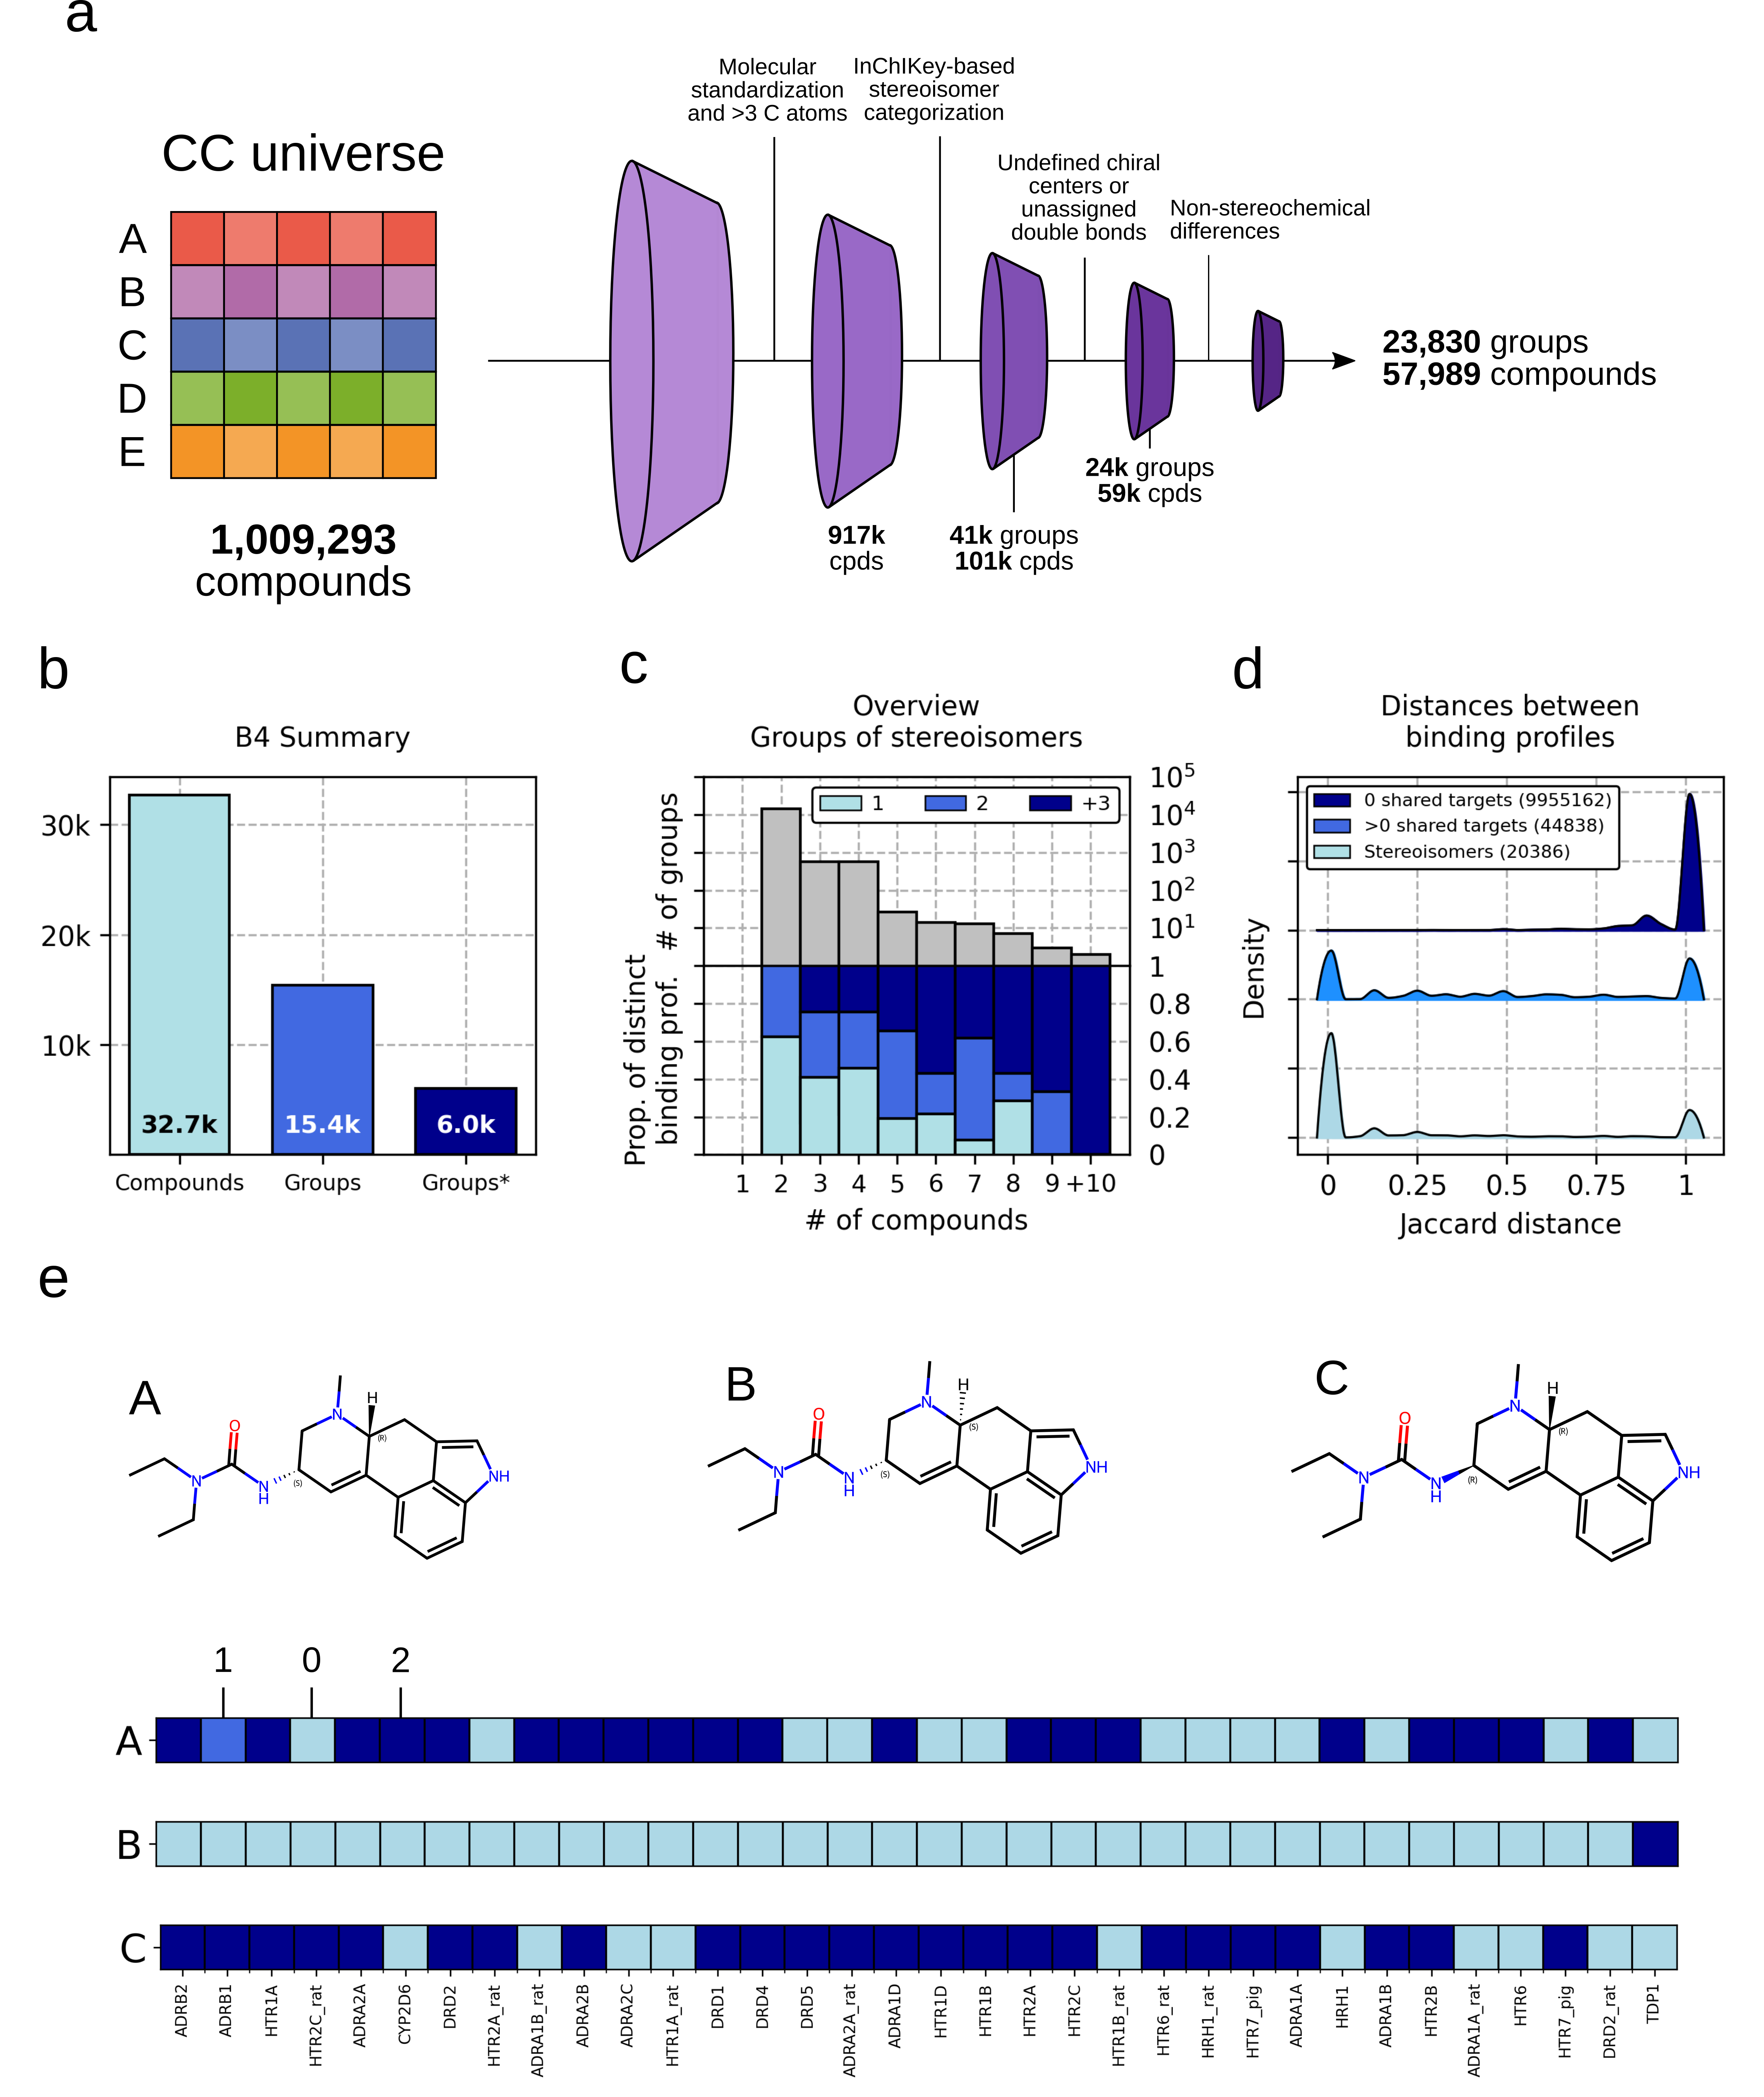
\includegraphics[width=1\linewidth]{figures/Stereoisomers/Main/Fig1_v2.png}
  \caption{
    \textbf{Stereoisomerism and bioactivity.}
    \textbf{a)} Computational pipeline to identify groups of stereoisomers in the CC chemical universe.
    \textbf{b)} Number of unique stereoisomeric compounds with experimentally identified protein targets in the CC B4 space, number of stereoisomer groups, and number of groups with at least 2 compounds with non-identical binding profiles.
    \textbf{c)} Number of groups (y-axis, top) having the specified number of stereoisomers (x-axis). Proportion of these groups (y-axis, bottom) having the specified number of distinct binding profiles (i.e. \textasciitilde60\% of the groups of 2 isomers have a unique binding profile).
    \textbf{d)} Distributions of Jaccard distances (binding profiles) between pairs of compounds sharing 0, ≥1 targets and stereoisomer pairs. All distributions are significantly different from each other (Mann-Whitney p-value\textasciitilde0).
    \textbf{e)} Illustrative example of a stereoisomer group including 3 small molecules with their corresponding target binding profiles, using the annotation of type 0 signatures (i.e. 0: no binding; 1: weak binding and 2: strong binding).
    \rule[0ex]{\textwidth}{0.5pt}
  }
  \label{Stereoisomers_Fig1}
\end{Figure_modified}
\subsection{Concluding remarks}


Bla bla bla


\subsection{Methods}


Bla bla bla

\newpage


%%%%%%%%%%%%%%%%%
%%% POCKETVEC %%%
%%%%%%%%%%%%%%%%%


\section{Chapter 3.4 -- Comprehensive detection and characterization of human druggable pockets through novel binding site descriptors}
% \addcontentsline{toc}{section}{Chapter 3.4 -- Comprehensive detection and characterization of human druggable pockets through novel binding site descriptors}
\renewcommand{\thefigure}{3.\arabic{section}.\arabic{figure}}

\subsection{Abstract}

Druggable pockets are protein regions that have the ability to bind organic small molecules, and their characterization is essential in target-based drug discovery. However, strategies to derive pocket descriptors are scarce and usually exhibit limited applicability. Here, we present PocketVec, a novel approach to generate pocket descriptors for any protein binding site of interest through the inverse virtual screening of lead-like molecules. We assess the performance of our descriptors in a variety of scenarios, showing that it is on par with the best available methodologies, while overcoming some important limitations. In parallel, we systematically search for druggable pockets in the folded human proteome, using experimentally determined protein structures and AlphaFold2 models, identifying over 32,000 binding sites in more than 20,000 protein domains. Finally, we derive PocketVec descriptors for each small molecule binding site and run an all-against-all similarity search, exploring over 1.2 billion pairwise comparisons. We show how PocketVec descriptors facilitate the identification of druggable pocket similarities not revealed by structure- or sequence-based comparisons. Indeed, our analyses unveil dense clusters of similar pockets in distinct proteins for which no inhibitor has yet been crystallized, opening the door to strategies to prioritize the development of chemical probes to cover the druggable space.

\subsection{Introduction}


Bla bla bla\cite{Eigen1971, Knuth1968}


%%% NUMBERING OF FIGURES %%%



\subsection{Methodological development and implementation}

It is known that similar proteins tend to bind similar ligands\cite{klabunde_chemogenomic_2007}, a principle behind many drug discovery projects\cite{sydow_advances_2019, keiser_relating_2007, falaguera_illuminating_2023}. We re-assessed the validity of this principle and found that, indeed, proteins from the same family (e.g. GPCRs) tend to have more similar active compounds than proteins from different families (Fig \ref{FigS1}). However, globally dissimilar proteins showing similar physicochemical and shape properties in their druggable pockets may still bind with similar ligands, which reasonably translates into a more precise and general form of the chemogenomics principle: similar pockets bind similar ligands\cite{gao_comprehensive_2013}. PocketVec builds on this observation to generate novel vector-type descriptors for characterizing protein small molecule binding pockets. 

Instead of directly characterizing the shape and physicochemical environment of the protein
cavities, we rely on a predefined set of small molecules and assess their potential binding to a
given pocket. More specifically, given a three-dimensional protein structure, we first identify
possible druggable pockets and we then use computational docking strategies to assess the
potential binding of the small molecules. The resulting docking scores are then translated into
rankings, which are finally stored in a vector-type format. In this way, each bit of the vector
represents the ranking of a predefined molecule, illustrating how good it binds with the pocket of
interest compared to all other molecules (Fig \ref{Fig1}). While the idea is conceptually pretty
straightforward, its implementation requires a thorough assessment of the set of used
molecules, the docking methodology and the benchmark strategy. The following sections
describe our effort to evaluate and optimize each step of the procedure.

%%%%%%%%%%%%%%%%
%%% FIGURE 1 %%%
%%%%%%%%%%%%%%%%

% \begin{figure}[htbp]
%   \centering
%   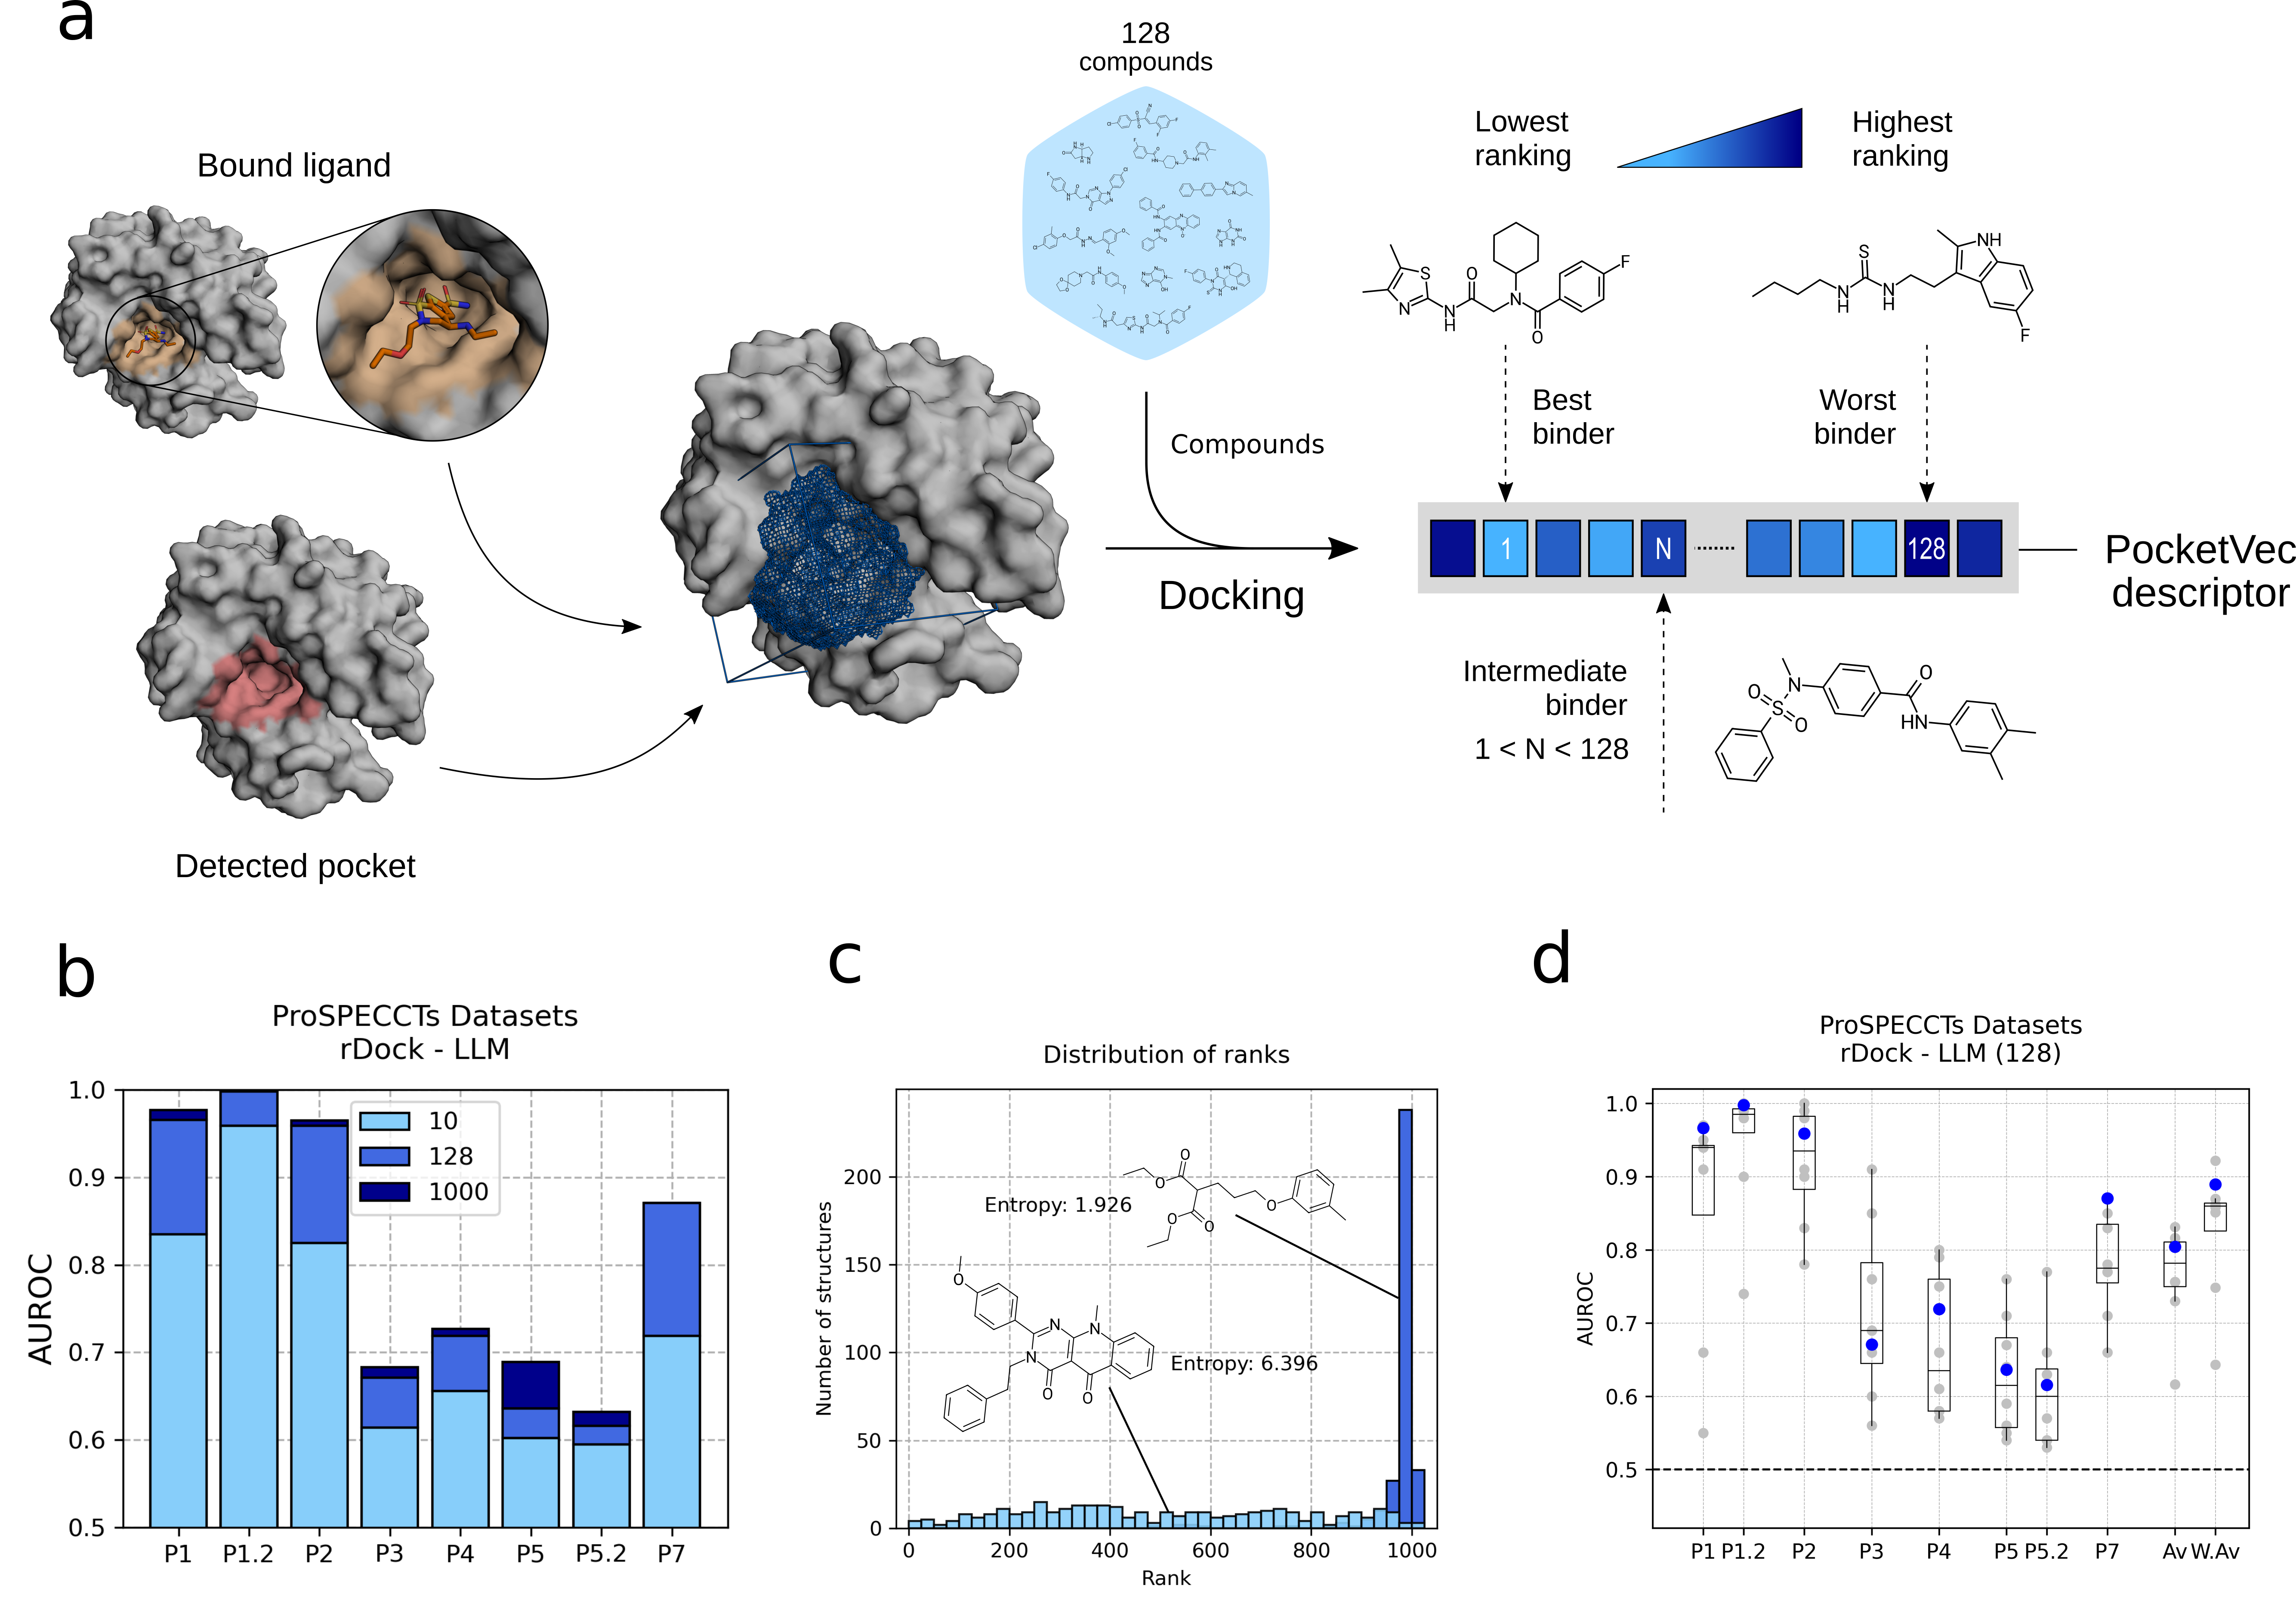
\includegraphics[width=\linewidth]{figures/PocketVec/Main/Fig1.png}
%   \caption{
%   Main title: PocketVec methodological pipeline and benchmark results. 
%   \begin{description}
%       \item[a] A
%       \item[b] A
%       \item[c] A
%       \item[d] A
%   \end{description}
%   }
%   \label{Fig1}
% \end{figure}

\begin{figure}[htbp]
  \centering
  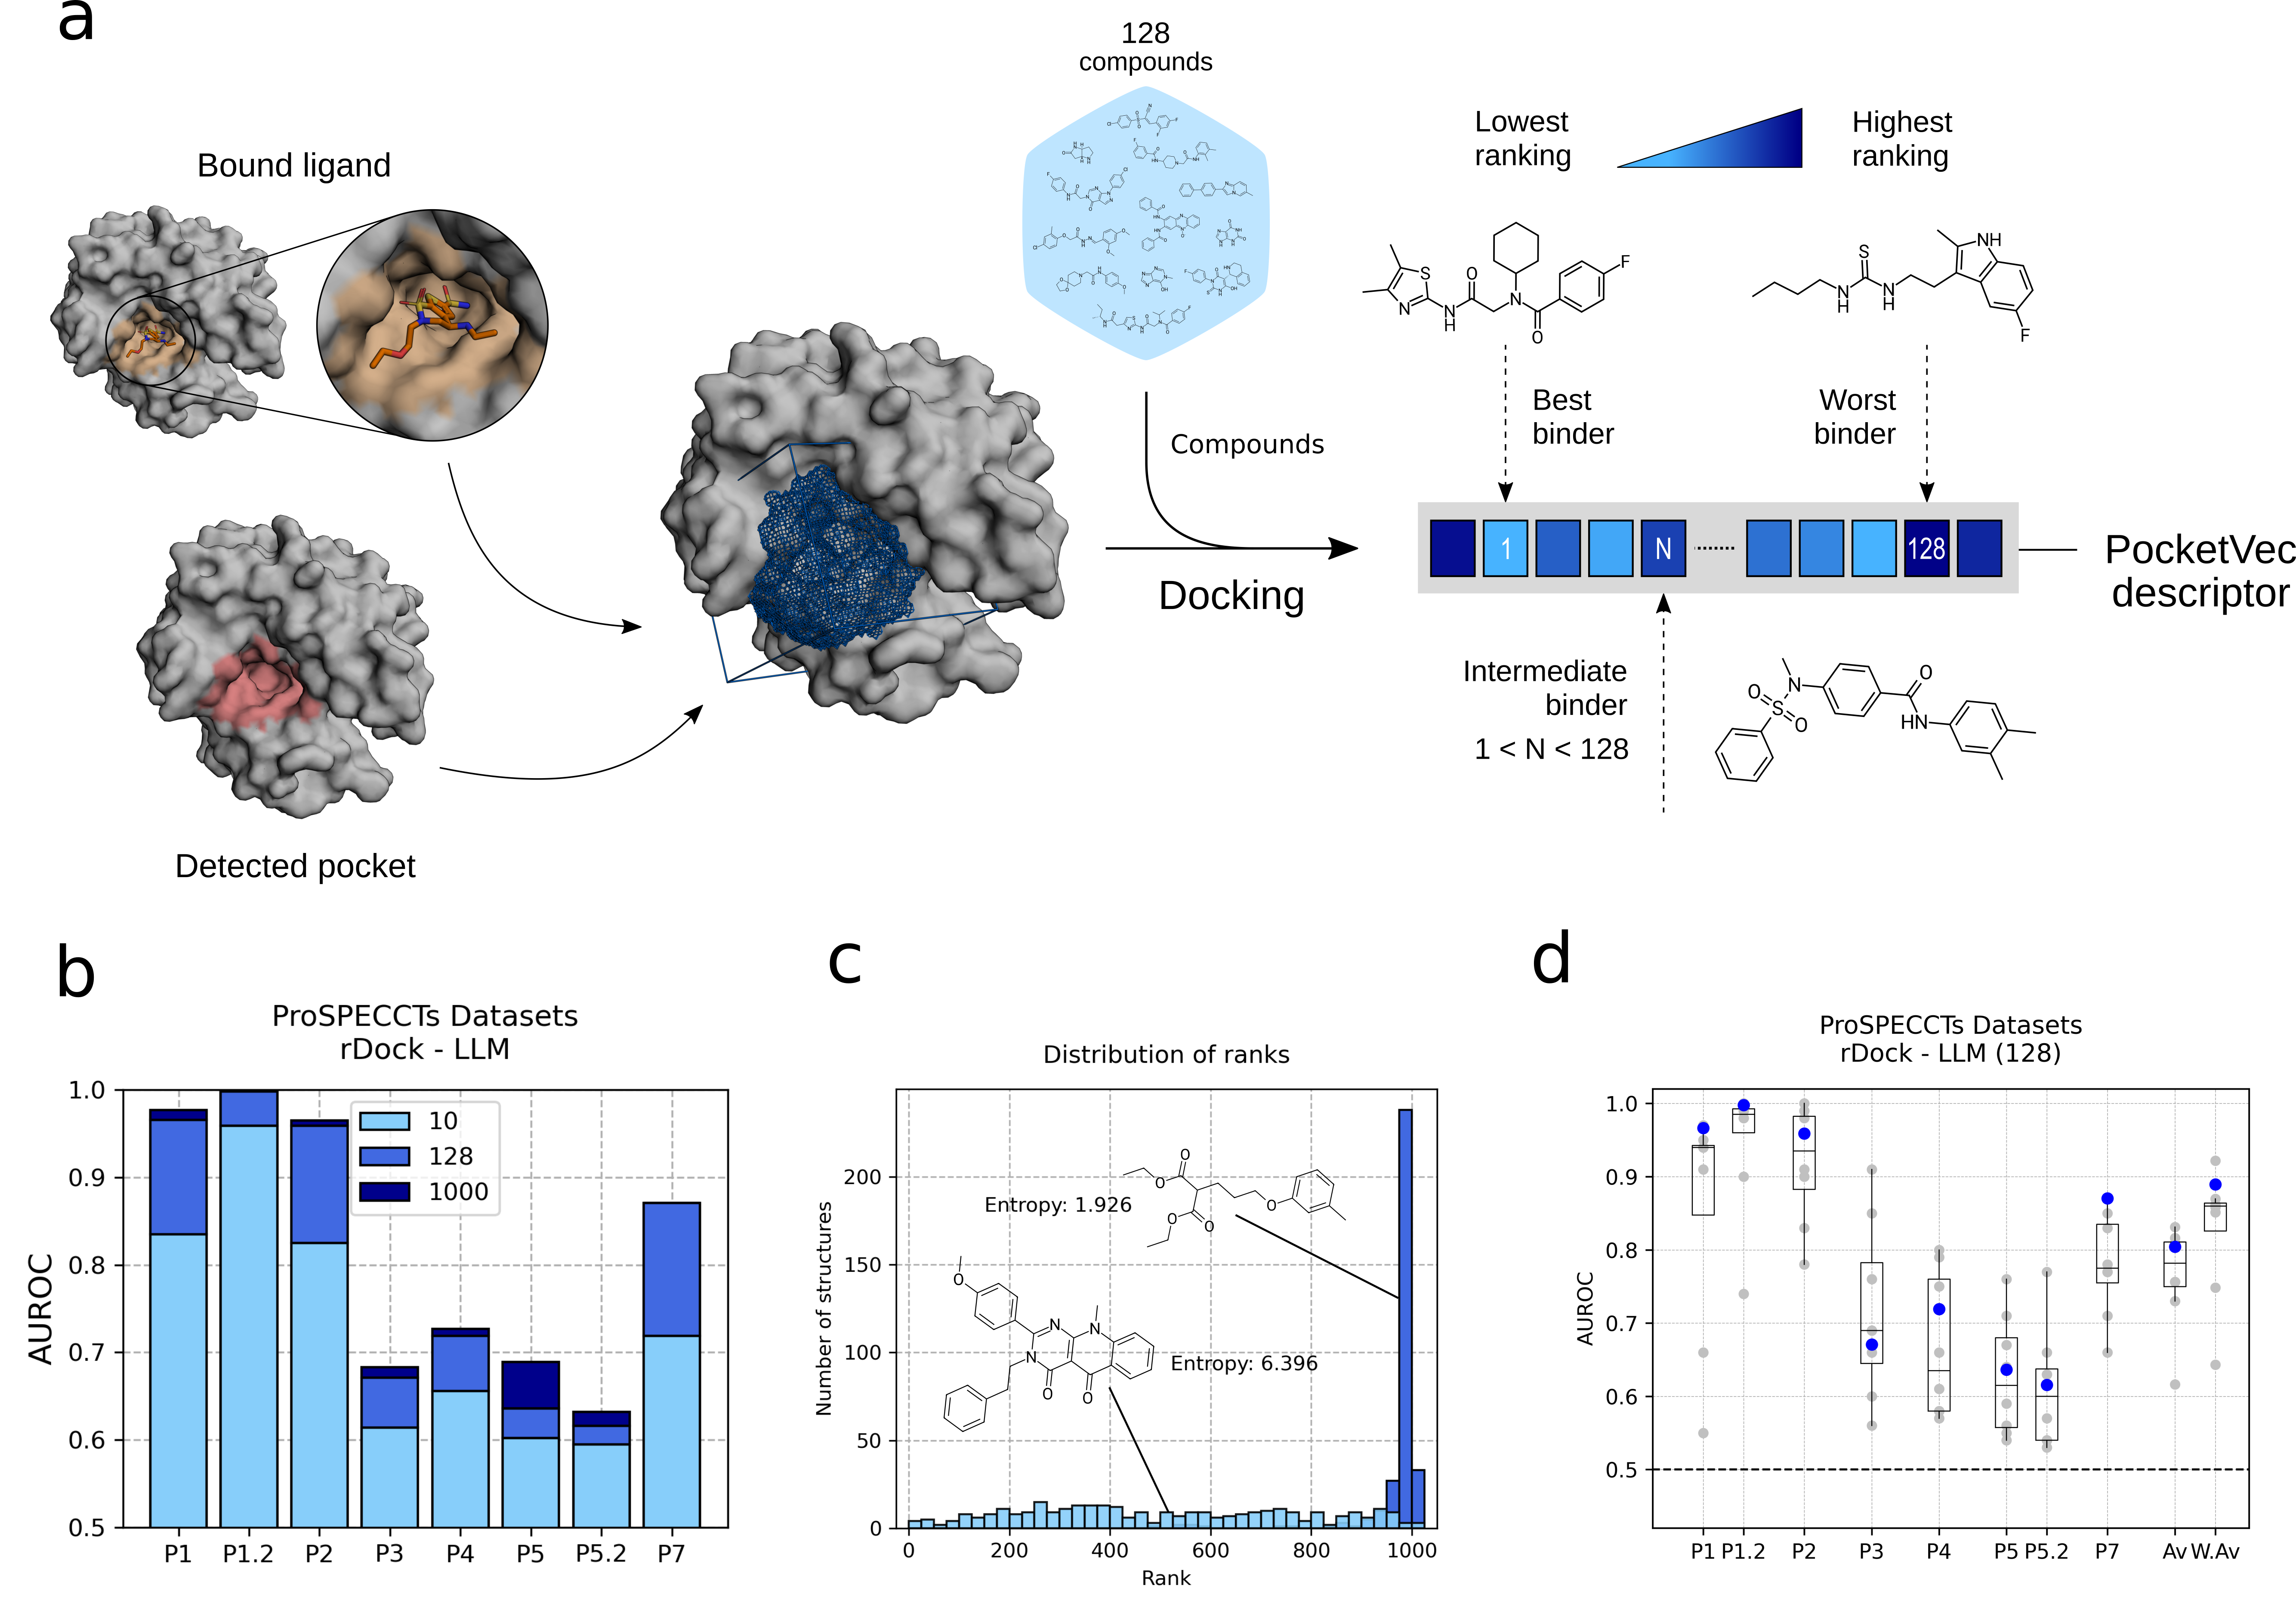
\includegraphics[width=\linewidth]{figures/PocketVec/Main/Fig1.png} 
  \caption{
    \textbf{PocketVec methodological pipeline and benchmark results.} 
    \textbf{a)} Given a 3D protein structure, binding site locations are established by the presence of bound ligands or by means of pocket detection algorithms. A predefined set of compounds (128 lead-like molecules in the standard PocketVec pipeline) is docked against the pocket of interest. The corresponding docking scores are then converted into rankings and stored in a vector-type format that serves to characterize the pocket. We refer to those vectors as PocketVec descriptors.
    \textbf{b)} Bars indicating the performance (AUROC, y-axis) of our descriptors generated with a varying number of predefined molecules among ProSPECCTs datasets (x-axis, P6 and P6.2 not included. For further details, please see Online Methods). Bar color indicates the number of predefined compounds (10, 128 and the complete set of 1,000 lead-like molecules, sorted by entropy). These results correspond to the rigid docking (rDock) and LLM combination. All the other combinations with all possible numbers of predefined compounds (from 1 to complete sets) are shown in Fig \ref{FigS7}.
    \textbf{c)} Predefined molecules with high and low entropy. The histograms depict the distribution (y-axis) of rankings (x-axis, bin width: 25) for the highest (sky blue) and lowest (dark blue) entropy lead-like molecules in ProSPECCTs P1. Their chemical structures are shown together with the corresponding entropy values.
    \textbf{d)} Performances (AUROC, y-axis) of distinct pocket descriptors among ProSPECCTs datasets (x-axis, P6 and P6.2 not included). Gray dots represent the individual performances of existing strategies to derive pocket descriptors (see Table \ref{TableS1}). Box plots indicate median (middle line), 25th, 75th percentile (box), and max and min value within the 1.5*25th and 1.5*75th percentile range (whiskers). Blue dots indicate the performance of PocketVec descriptors (128 LLM and rDock rigid docking). Av. values represent the average performance among ProSPECCTs datasets for each individual method and W. Av. values weight the average value according to the number of pairs within each dataset.
  }
  \label{Fig1}
\end{figure}
\subsection{Results and discussion}

%%%%%%%%%%%%%%%%%%%%%%%%%%%%%%%%%%%%%%%%%%%%%%%%%%%%%%%%%%%%%%%%
%%  PocketVec performance on the ProSPECCTs benchmark sets  %%%%
%%%%%%%%%%%%%%%%%%%%%%%%%%%%%%%%%%%%%%%%%%%%%%%%%%%%%%%%%%%%%%%%

\phantomsection
\subsubsection{PocketVec performance on the ProSPECCTs benchmark sets}
\label{PocketVec_ResultsAndDiscussion_PocketVec_performance_on_the_ProSPECCTs_benchmark}

The performance of PocketVec descriptors across ProSPECCTs datasets is assessed in terms of the AUROC and is shown in Fig \ref{PocketVec_Fig1}d. We observe that PocketVec descriptors are robust to varying definitions of the same pocket, as determined by different crystallized ligands (P1, AUROC 0.97). When restricting such definitions to chemically similar ligands, the performance is maximal (P1.2, AUROC 1.00). Similarly, our descriptors are robust against protein conformational changes, i.e. protein flexibility (P2, AUROC 0.96), and they are also able to distinguish identical pockets from those altered by 5 artificial mutations leading to changes in physicochemical and shape properties of pocket-lining residues. In these cases, we obtained more modest performances (P3--physicochemical changes and P4--both physicochemical and shape changes, AUROCs of 0.67 and 0.72, respectively). Reassuringly though, we observed a significant correlation between the number of artificial mutations (1 to 5) and the corresponding AUROC values (Pearson CC > 0.98, p-value < 0.005 in both P3 and P4, Fig \ref{PocketVec_FigS9}), which confirmed that an increasing number of mutations in the binding site came along with an improved ability to detect such differences using PocketVec descriptors. 

We also benchmarked our descriptors in more biologically relevant scenarios where, for instance, pockets binding similar small molecules are found in structurally different proteins. ProSPECCTs includes two datasets to address such cases: P5 includes pocket structures classified into 9 distinct ligand classes (e.g. HEM, ATP, NAD, etc.), and P7 includes a realistic set of binding site pairs reported to be similar in published literature, some of them identified in otherwise unrelated proteins. In these sets, PocketVec descriptors show performances with AUROCs of 0.64 and 0.87, respectively, demonstrating their ability to identify similar pockets in globally dissimilar proteins. It is important to note that two binding sites having identical (or chemically similar) crystallized ligands are not necessarily similar from a PocketVec perspective. Following the logic behind the similarity ensemble approach (SEA\cite{keiser_relating_2007}), in which targets are quantitatively compared based on the chemical similarity of the ensemble of their ligands, a pair of targets sharing a single active compound may not be significantly similar.

Finally, with the goal of defining a PocketVec distance threshold to classify any pocket pair of interest as either similar or dissimilar, we analyzed the behavior of the Matthew's Correlation Coefficient (MCC) at multiple cut-off values across the different ProSPECCTs datasets (Fig \ref{PocketVec_FigS10}). As expected, each definition of pocket similarity in the ProSPECCTs datasets suggested the choice of a different cut-off distance. For instance, the optimal cut-off in the mutation-related benchmarks (P3 and P4) was around 0.13, while in the most realistic set of binding site pairs reported to be similar in published literature was even lower, around 0.08. However, for general purposes and to minimize false negatives, we selected the distance threshold based on the P1 dataset, where similar pairs were predefined as identical pockets binding chemically distinct ligands whereas dissimilar pairs were unrelated pockets binding different ligands. In this way, we defined 0.17 as our PocketVec threshold distance, which was the value maximizing the MCC in ProSPECCTs P1. However, this threshold should not be regarded as an absolute standard, but rather as a general guideline for classifying a pocket pair of interest as either similar or dissimilar.

For the sake of completeness, we generated results for all combinations of docking methods (rigid--rDock, and flexible--SMINA) and reduced sets of chemical compounds (128 LLM and 128 fragments). The use of rDock and LLM (128) was still the best strategy according to the ProSPECCTs datasets (Fig \ref{PocketVec_FigS11}). Besides, we observed that the selection of compounds leading to the most variable results throughout the different pockets (i.e. high entropy) was, indeed, of great help to distinguish similar from dissimilar pockets in ProSPECCTs P1. This effect was even more pronounced in the fragments, where their lower complexity and molecular weight led to higher promiscuity and redundancy (Fig \ref{PocketVec_FigS12}).

Detailed plots for all ProSPECCTs datasets including ROC Curves, PR Curves and distributions of PocketVec distances, docking scores and pocket volumes are included in our \hl{GitLab repository} (see \hyperref[PocketVec_Code]{Code and data availability}). 



%%%%%%%%%%%%%%%%%%%%%%%%%%%%%%%%%%%%%%%%%%%%%%%%%%%%%%%%%%%%%%%%
%%%%%%%%%%  Comparison with existing strategies  %%%%%%%%%%%%%%%
%%%%%%%%%%%%%%%%%%%%%%%%%%%%%%%%%%%%%%%%%%%%%%%%%%%%%%%%%%%%%%%%

\phantomsection
\subsubsection{Comparison with existing strategies}
\label{PocketVec_ResultsAndDiscussion_Comparison_with_existing_strategies}

Next, we compared the performance of PocketVec descriptors with state-of-the-art methodologies, as reported in several studies\cite{simonovsky_deeplytough_2020, scott_classification_2022, ehrt_benchmark_2018}, where the authors benchmarked many pocket comparison tools against the ProSPECCTs datasets, including six strategies based on pocket descriptors (Fig \ref{PocketVec_Fig1}d and Fig \ref{PocketVec_FigS11}). We used the AUROC as the standard performance measure to be able to compare our results with other available methodologies. However, for PocketVec descriptors, we also provide specific values of precision, accuracy, sensitivity, specificity, Matthew´s correlation coefficient and F1 score in each ProSPECCTs dataset (Fig \ref{PocketVec_FigS13}). Overall, PocketVec is the second-best ranked strategy in terms of the weighted average among datasets (0.89) and, indeed, it surpasses the median and the average performance in all ProSPECCTs datasets, apart from P3 (Table \ref{PocketVec_TableS1}). The top-scoring method is SiteAlign\cite{schalon_simple_2008}, which is alignment-dependent and based on the projection of residue descriptors into a triangle-discretized sphere that quantifies binding site similarity by minimizing distances between systematically generated cavity fingerprints obtained by moving one binding site with respect to the other. Thus, being specifically developed to compare pockets, it does not provide a unique descriptor for each binding site, which hampers the exploration of the pocket space in the same way molecular fingerprints do for the chemical space of small molecules. \hl{START} Other strategies are indeed alignment-free and provide unique representations for binding sites but, in addition to showing worse performances than PocketVec descriptors among ProSPECCTs datasets, also present several intrinsic limitations. For instance, KRIPO\cite{wood_pharmacophore_2012} and TIFP\cite{desaphy_encoding_2013} characterize protein-ligand binding interactions between receptors and bound ligands, which enables the identification of shared interaction patterns between pockets but limits their applicability domain to \textit{holo} structures. Additionally, FuzCav\cite{weill_alignment-free_2010} fingerprints count for specific pharmacophoric triplets of pocket-lining Cα, which enables the use of \textit{apo} structures but imply a simplistic representation of pockets. On a different note, Deeplytough\cite{simonovsky_deeplytough_2020} and BindSiteS-CNN\cite{scott_classification_2022} generate pocket descriptors by means of deep learning strategies, which makes them strongly dependent on training data and provide pocket embeddings that are difficult to interpret. \hl{END} Thus, overall, PocketVec represents a fast strategy to generate accurate pocket descriptors that overcome the aforementioned limitations, and it shows a higher performance at assessing pocket similarities than most current strategies (Fig \ref{PocketVec_FigS14}).




%%%%%%%%%%%%%%%%%%%%%%%%%%%%%%%%%%%%%%%%%%%%%%%%%%%%%%%%%%%%%%%%
%%% Comprehensive characterization of druggable pockets in the human proteome
%%%%%%%%%%%%%%%%%%%%%%%%%%%%%%%%%%%%%%%%%%%%%%%%%%%%%%%%%%%%%%%%

\phantomsection
\subsubsection{Comprehensive characterization of druggable pockets in the human proteome}
\label{PocketVec_ResultsAndDiscussion_Comprehensive_characterization}

PocketVec descriptors constitute an optimal framework to comprehensively characterize large and diverse sets of small molecule binding sites (\textit{apo}/\textit{holo} structures), enabling the navigation across the pocket space of complete proteomes. In view of this, we designed a computational pipeline to generate PocketVec descriptors for all pockets included within human protein domains (Fig \ref{PocketVec_Fig2}a). Please, see \hyperref[PocketVec_Methods]{Methods} for a detailed description of the strategy.

%%%%%%%%%%%%%%%%
%%% FIGURE 2 %%%
%%%%%%%%%%%%%%%%


\begin{figure}[H]
  \centering
  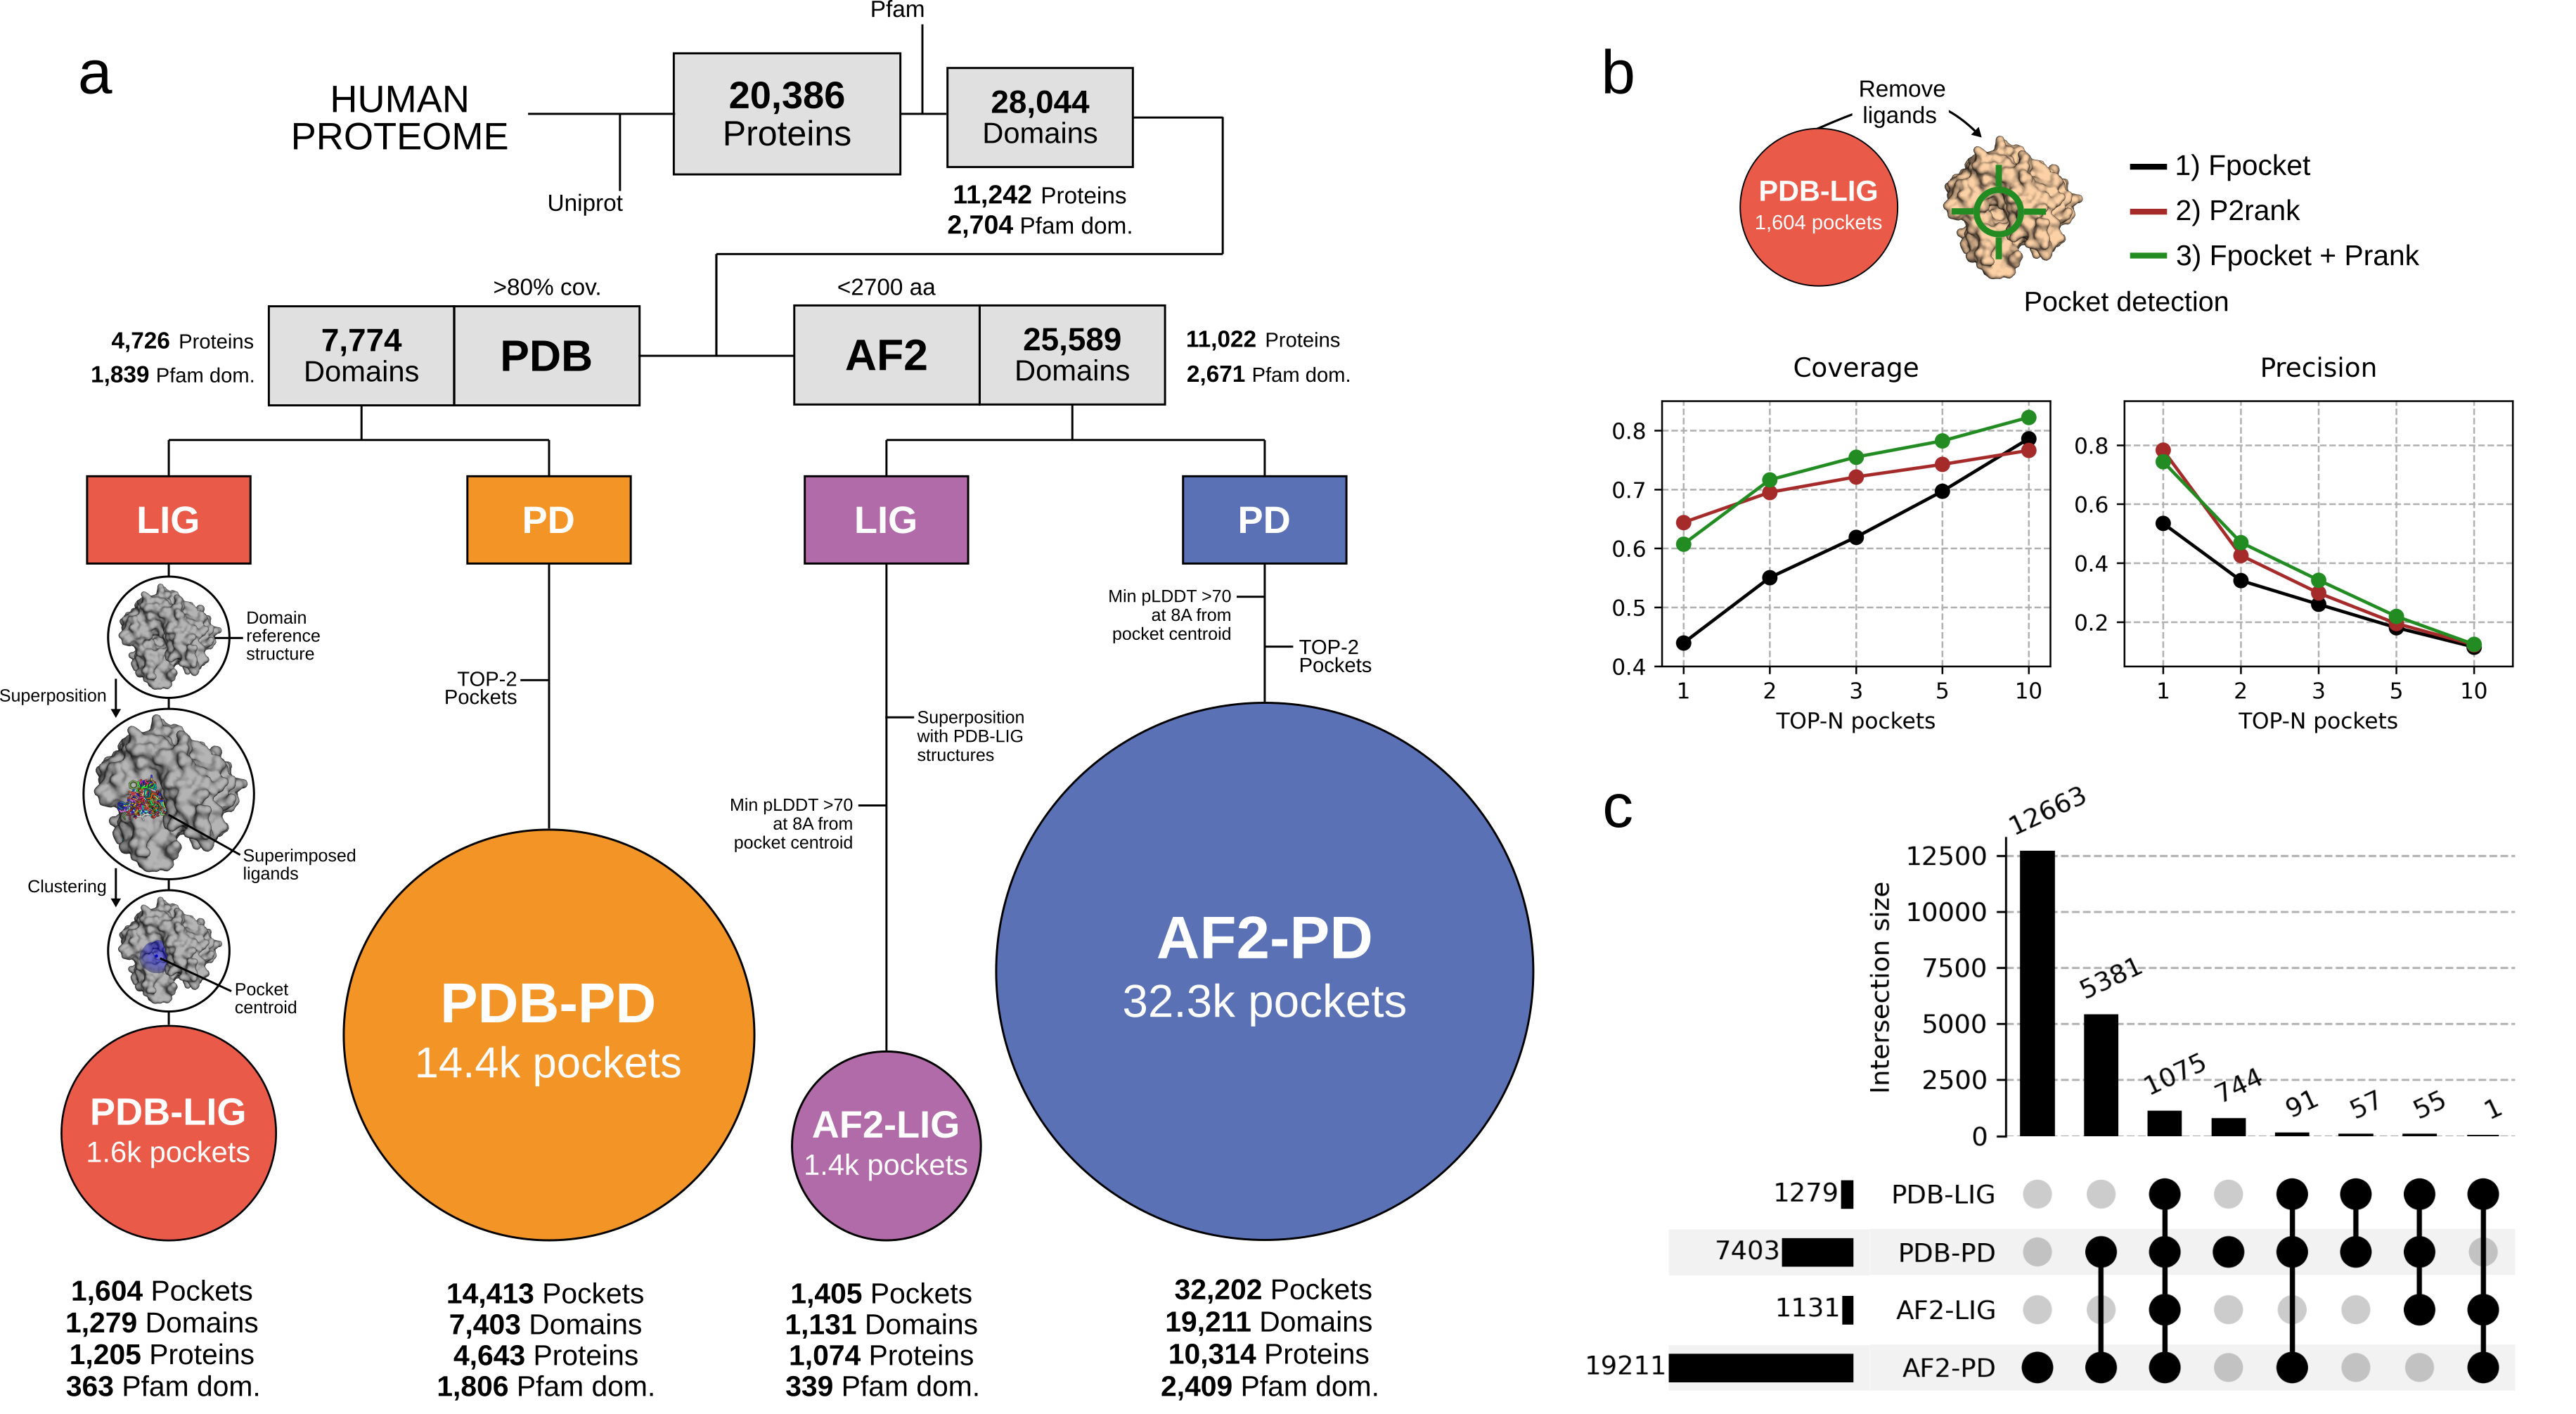
\includegraphics[width=\linewidth]{figures/PocketVec/Main/Fig2.png} 
  \caption{
    \textbf{Generating PocketVec descriptors for all druggable pockets within human protein domains.} 
    \textbf{a)} Computational pipeline to gather all available structural data for human druggable pockets included within protein Pfam domains. Starting from the complete human proteome as per Uniprot, we first identified Pfam domains in experimentally determined structures (PDB) and AF2 predicted models. For PDB structures, we identified pockets in \textit{holo} domain structures based on the position of co-crystallized ligands (1,604 PDB-LIG pockets, red) and in \textit{apo} domain structures using pocket detection techniques (14,413 PDB-PD pockets, orange). We defined ligand-based pockets on AF2 structures (1,405 AF2-LIG pockets, purple) by directly superimposing the location of PDB-LIG pockets, and pockets were also predicted in AF2 models by means of pocket detection algorithms (32,202 AF2-PD pockets, blue).  For additional details about the pipeline, please consult the text and the \hyperref[PocketVec_Methods]{Methods} section.
    \textbf{b)} Benchmark of 3 distinct pocket detection strategies: Fpocket (black), P2rank (brown) and the combination of Fpocket and Prank (green). First, we removed bound ligands from reference PDB structures (PDB-LIG) and we then assessed the performance of the mentioned strategies to detect pockets in ligand-free structures. The plots below represent the evolution of Coverage (proportion of real pockets that are actually detected) and Precision (proportion of detected pockets that are actually real -have a crystallized ligand on PDB-LIG) in terms of the number of best-scoring detected pockets per domain that are considered (1, 2, 3, 5 and 10).
    \textbf{c)} UpSet plot representing the intersecting number of domains among pocket sets (1,279 domains in PDB-LIG, 7,403 domains in PDB-PD, 1,131 domains in AF2-LIG and 19,211 domains in AF2-PD).
  }
  \label{PocketVec_Fig2}
\end{figure}


In brief, we first retrieved all 20,386 human proteins in UniProt\cite{the_uniprot_consortium_uniprot_2023}. To avoid working with unstructured or very flexible regions, difficult to model and unlikely to contain druggable pockets, we only kept those protein sequences within autonomous structural units (i.e. domains), as defined in Pfam\cite{mistry_pfam_2021}. Overall, we kept 28,044 domains (2,704 unique Pfam domains) in 11,242 human proteins (Fig \ref{PocketVec_FigS15}). The next step was to structurally annotate these domains, for which we used two different strategies. On the one hand, we looked for experimentally determined structures searching the PDB\cite{goodsell_rcsb_2020}, identifying at least one PDB structure for 7,774 domains (1,839 unique Pfam domains in 4,726 proteins). Additionally, we downloaded all human predicted protein structures from AlphaFold DB, obtaining structural models for 25,589 domains (2,671 unique Pfam domains in 11,022 proteins). There is an ongoing debate on the use of AF2 models for docking experiments, and whether such models should be refined using e.g. molecular dynamics simulations. However, most studies suggest that the accuracy of AF2 models in docking experiments is comparable to experimentally determined \textit{apo} structures (i.e. without a ligand bound)\cite{zhang_benchmarking_2023, holcomb_evaluation_2023, scardino_how_2023}. Indeed, it has been recently shown that the experimental validation rates of small molecule docking are indistinguishable when PDB structures or AF2 models are used\cite{lyu_alphafold2_2023}.

Next, for each domain, we identified the potentially druggable pockets, also using two different strategies. In the first one, that we termed \textit{ligand-based} pocket definition, we searched for small molecules co-crystallized together with the protein domain, and defined druggable pockets as those having bound compounds (HET PDB codes) fulfilling the following criteria: i) being annotated as such in PDBSUM data, ii) not being one of the 20 naturally occurring amino acids, iii) having more than 6 carbon atoms, to filter out solvent molecules and crystallography-related species and iv) having solvent accessibility ≤0.4 or buriedness ≥15 (\hyperref[PocketVec_Methods]{Methods}). In total, we found at least one PDB structure containing small molecules for 1,279 domains (363 unique Pfam domains in 1,205 proteins). For 503 of these, we only found a single ligand fulfilling our criteria, whereas for 254 of them we could find 10 or more ligands (Fig \ref{PocketVec_FigS16}). Then, to compile the list of unique ligand-defined pockets, we chose a reference PDB structure for each protein domain, and superimposed all domain structures with the corresponding bound ligands onto the reference. We then used a single-linkage clustering strategy to merge into a single pocket all those ligands whose centroids were at a distance ≤5Å while maintaining the maximum distance between the global centroid of the cluster and the centroids of the individual compounds ≤18Å. We considered the final global cluster centroids as the pocket centroids. Overall, we found 1,604 ligand-defined pockets in 1,279 protein domains (363 unique Pfam domains in 1,205 proteins). We named this set of pockets \textbf{PDB-LIG}. To apply the same criteria to those structures modeled with AF2, for each domain, we superimposed the reference PDB structure onto the AF2 model, and transferred the location of the identified PDB-LIG pockets accordingly. We only considered those pockets having a pLDDT value >70 for all residues at a distance ≤8Å from the pocket centroid. In total, we identified 1,405 pockets in 1,131 domains (339 unique Pfam domains in 1,074 proteins), and named this set \textbf{AF2-LIG}. As a complementary strategy, and to increase the overall coverage of the human pocketome, we attempted a de novo identification of druggable pockets. To find the most accurate strategy to predict druggable pockets, we assessed the accuracy of different methods at identifying the PDB-LIG pockets defined above. In brief, we first removed bound ligands from reference \textit{holo} structures and used Fpocket\cite{le_guilloux_fpocket_2009} and P2rank\cite{krivak_p2rank_2018}, to detect pockets in ligand-free domain structures (\hyperref[PocketVec_Methods]{Methods}). Our benchmark showed that the best strategy to detect binding sites in ligand-free structures was the combination of Fpocket, for pocket detection, and Prank to score them. Using this combination, and considering the top-2 best scored pockets for each domain, we were able to detect 72\% of the real pockets while 47\% of detected pockets were indeed real (Fig \ref{PocketVec_Fig2}b, coverage and precision, respectively). Thus, for each domain, we ran Fpocket on the PDB reference structure to identify potential pockets, we ranked them by means of Prank, and we kept the top-2 ranked pockets per domain. Overall, this accounted for a total of 14,413 predicted pockets in 7,403 domains (1,806 unique Pfam domains in 4,643 proteins). We named this set \textbf{PDB-PD}. We then used the same strategy and criteria as before to detect pockets onto the predicted AF2 domain models, annotating a total of 32,202 pockets in 19,211 domains (2,409 unique Pfam domains in 10,314 proteins). We named this set \textbf{AF2-PD}.



%%%%%%%%%%%%%%%%%%%%%%%%%%%%%%%%%%%%%%%%%%%%%%%%%%%%%%%%%%%%%%%%
%%% Robustness in the detection of druggable pockets
%%%%%%%%%%%%%%%%%%%%%%%%%%%%%%%%%%%%%%%%%%%%%%%%%%%%%%%%%%%%%%%%

\phantomsection
\subsubsection{Robustness in the detection of druggable pockets}
\label{PocketVec_ResultsAndDiscussion_Robustness_Detection}

Globally, using the different strategies to structurally annotate human protein domains and to identify validated and potential druggable pockets, we compiled 1,604 PDB-LIG, 1,405 AF2-LIG, 14,413 PDB-PD and 32,202 AF2-PD druggable pockets, in 20,067 domains (Fig \ref{PocketVec_Fig2}a and Fig \ref{PocketVec_Fig2}c). The significant added value of \textit{de novo} methodologies is very apparent. Indeed, for 18,788 domains (93.6\%), all pockets were identified only with pocket detection strategies and, among these, 12,663 domains (63.1\%) exclusively featured pockets on AF2 models (Fig \ref{PocketVec_Fig2}c).

Interestingly, when we assessed the methodological robustness of pocket predictions using a subset of 1,000 PDB-PD domains, we observed that results slightly differed after translating and rotating structures. This effect was observed for both PDB and AF2 structures in a consistent manner: only \textasciitilde85\% and \textasciitilde86\% of detected pockets were evenly identified after rotation and translation, respectively (top-2 pockets, Fig \ref{PocketVec_FigS17}a). However, in the pockets identified regardless of variations in the initial structures, the scoring was very consistent both in PDB structures and AF2 models (Pearson CC \textasciitilde0.98). We also evaluated the coherence between pockets detected in PDB and AF2 structures, finding that only \textasciitilde59\% and \textasciitilde49\% of detected pockets were evenly identified in PDB and AF2 structures with respect to a reference PDB structure. However, as when comparing discrepancies due to different initial orientations, in the pockets identified both in PDB and AF2 structures the scoring was quite robust, with Pearson CC of \textasciitilde0.88 and \textasciitilde0.62 for PDB and AF2 models, respectively (Fig \ref{PocketVec_FigS17}b). 

Additionally, we also explored potential differences in the physicochemical properties between the real (ligand-defined) and predicted (detected) pockets, comparing their volumes and buriedness values (see \hyperref[PocketVec_Methods]{Methods}). In this case, as the only remarkable difference, we found that real pockets identified from bound ligands tended to be smaller than those predicted in the PD framework, with average volumes of \textasciitilde3,000 Å3 and \textasciitilde3,800 Å3 for LIG and PD pockets, respectively (Fig \ref{PocketVec_Fig3}a). As expected, we reached the same conclusion with buriedness values (Fig \ref{PocketVec_FigS18}), since pocket volume and buriedness were indeed negatively correlated (Fig \ref{PocketVec_FigS19}).

Altogether, these results underscore some limitations in the pocket detection strategy, revealing slight variations due to the orientation of the initial structures, a stronger dependence on structural variability and the production of predicted pockets whose physicochemical properties (e.g. volume) diverge from known pockets. 


%%%%%%%%%%%%%%%%
%%% FIGURE 3 %%%
%%%%%%%%%%%%%%%%

\begin{figure}[htbp]
  \centering
  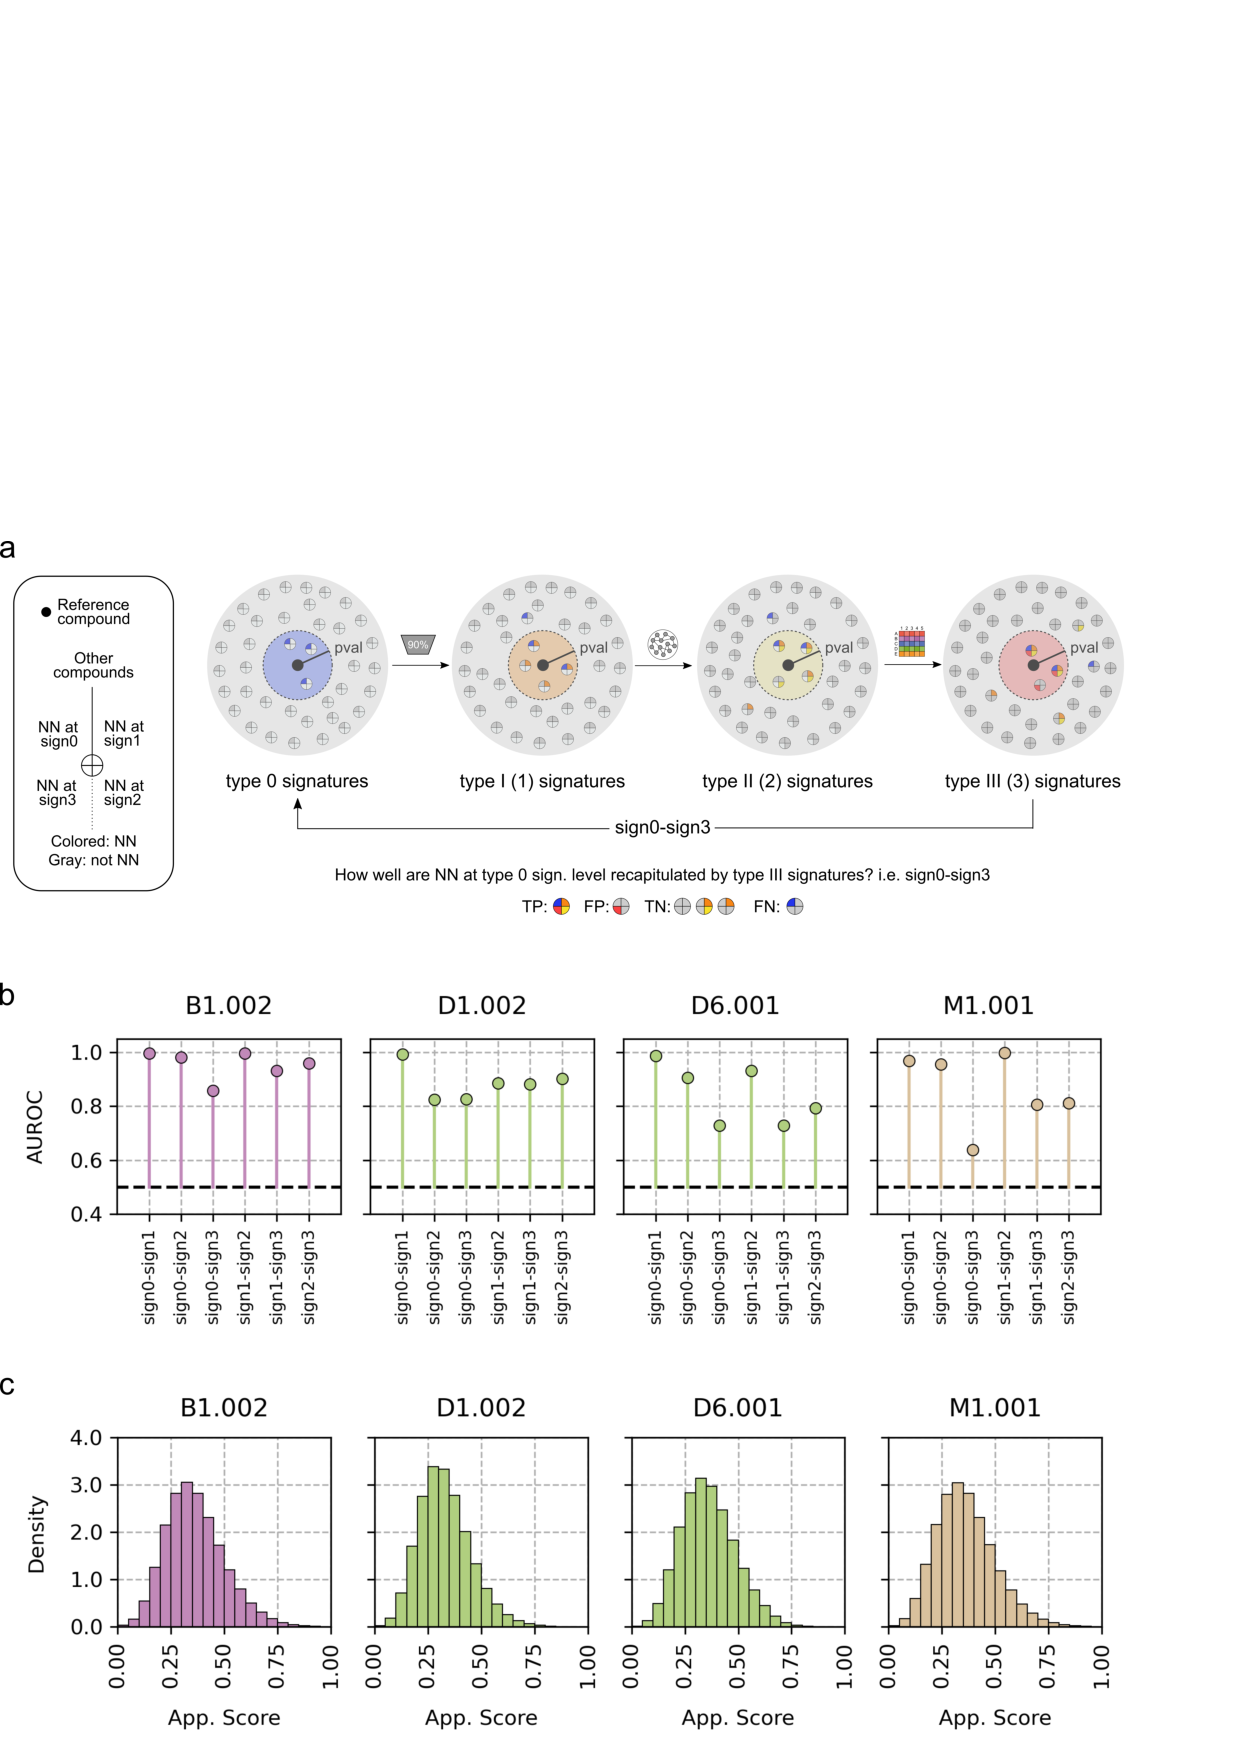
\includegraphics[width=\linewidth]{figures/PocketVec/Main/Fig3.png}
  \caption{
    \textbf{Characterization of human druggable pockets using PocketVec descriptors.} 
    \textbf{a)} Distribution of volumes (x-axis, x10³ A³) for each pocket set: PDB-LIG (1,604 pockets, red), PDB-PD (14,413 pockets, orange), AF2-LIG (1,405 pockets, purple) and AF2-PD (32,302 pockets, blue). All distributions are normalized (density, y-axis). The average volumes are 2992.88 A³, 3764.1 A³, 2940.47 A³ and 3972.66 A³, respectively. Pocket volumes were directly calculated using the rDock\cite{ruiz-carmona_rdock_2014} CAVITY functionality. 
    \textbf{b)} Correlation between average docking rankings among all pocket sets. For each pocket set, a 128-length array containing the average docking ranking for each lead-like molecule was calculated, and these arrays were compared among pocket sets by means of the Pearson’s Correlation Coefficient. All p-values (10) are <10\textsuperscript{-25}. 
    \textbf{c)} For each pocket set, proportion of PocketVec descriptors (\%, y-axis) having less than N (x-axis) outlier molecules (i.e. molecules with positive docking scores, please see \hyperref[PocketVec_Methods]{Methods}).
    \textbf{d)} Proportion of originally dissimilar pocket pairs (y-axis, distances >threshold) classified as similar (distances <threshold) due to the artificial insertion of a growing number of outlier values (x-axis) at different distance thresholds. To run the analysis, 100,000 PocketVec distances were randomly sampled (x10 times) from PDB-LIG. Solid lines represent average results and shadowed areas correspond to minimum and maximum proportions among samples. Results did not change among pocket sets (Fig \ref{PocketVec_FigS23}).
    \textbf{e)} tSNE (t-distributed Stochastic Neighbor Embedding) representation of all PocketVec descriptors within each pocket set (PDB-LIG, PDB-PD, AF2-LIG, AF2-PD). Each pocket is represented by a single point, which is colored and sized by 2D density within the pocket set. Gray dots correspond to the background space: all PocketVec descriptors are considered at once, and are also colored and sized by 2D density.
    \textbf{f)} Distributions (density, y-axis) of maximum Tanimoto Similarity among bound ligands (x-axis, bin width: 0.02) grouped by PocketVec distance ranges (0-0.10, 0.10-0.17 and 0.17-0.4). The number of pocket pairs per PocketVec distance range is specified in parenthesis.
    \textbf{g)} Distributions (density, y-axis) of PocketVec cosine distances (x-axis) grouped by the maximum Tanimoto Similarity among bound ligands (0-0.5, 0.5-0.8, 0.8-1 and 1). The number of pocket pairs per maximum Tanimoto Similarity range is specified in parenthesis.
    \textbf{h)} Distributions (density, y-axis) of PocketVec cosine distances (x-axis) grouped by the number of shared ligands between pockets (0, 1, 2 and 3 or more). The number of pocket pairs per number of shared ligands is specified in parenthesis.
  }
  \label{PocketVec_Fig3}
\end{figure}


%%%%%%%%%%%%%%%%%%%%%%%%%%%%%%%%%%%%%%%%%%%%%%%%%%%%%%%%%%%%%%%%
%%% Systematic generation of PocketVec descriptors
%%%%%%%%%%%%%%%%%%%%%%%%%%%%%%%%%%%%%%%%%%%%%%%%%%%%%%%%%%%%%%%%

\phantomsection
\subsubsection{Systematic generation of PocketVec descriptors}
\label{PocketVec_ResultsAndDiscussion_Systematic_generation_of_PocketVec_descriptors}


Once we had identified human druggable pockets with four different approaches, we systematically generated PocketVec descriptors for all of them, using the strategy described above (Fig \ref{PocketVec_Fig1}a). The high number of pockets explored enabled an exhaustive analysis of potential dependencies between the lead-like molecules used to build the descriptors and the characterization of druggable pockets. Reassuringly, we did not find any correlation between docking rankings and molecular properties of docked compounds (e.g. molecular weight or number of heavy atoms, Fig \ref{PocketVec_FigS20} and Fig \ref{PocketVec_FigS21}, respectively). On the contrary, we observed that most molecules exhibited a complete range of rankings (from 1 to 128), although the ranking distributions showed that some molecules tended to bind with good scores in many pockets while others were mostly downranked (Fig \ref{PocketVec_FigS22}). Indeed, this tendency was observed in all pocket definition strategies, and we found significant correlations between the average docking rankings for docked lead-like molecules among different pocket sets (Fig \ref{PocketVec_Fig3}b). Such correlations showed a perfect agreement between PocketVec descriptors generated through PDB and AF2 structures, but exposed slight differences between LIG and PD results (Fig \ref{PocketVec_Fig3}b, Pearson’s CC <0.88). In line with this, we found that 88.0\% and 86.8\% of the PocketVec descriptors generated for PDB-LIG and AF2-LIG, respectively, showed no lead-like molecules with positive docking scores (i.e. outlier molecules not fitting in the pocket, see \hyperref[PocketVec_Methods]{Methods}), while the fraction was considerably higher in PDB-PD and AF2-PD sets, with 97.0\% and 98.1\% of the descriptors, respectively (Fig \ref{PocketVec_Fig3}c). This result was consistent with the differences observed in pocket volumes (Fig \ref{PocketVec_Fig3}a). Reassuringly, we found that smaller pockets (<3,000ų) tended to be more prone to exhibit outlier molecules than bigger pockets (Fisher exact test, OR >70 and p-value <10\textsuperscript{-45} for all pocket sets).


To assess if outlier compounds could have a significant effect in the generation of poor PocketVec descriptors, we randomly inserted outlier values in the descriptors and computed the fraction of originally dissimilar pocket pairs (PocketVec distance >0.17) that were incorrectly labeled as similar (distance <0.17) due to an increasing number of outlier values. We observed that the insertion of up to 80 outlier molecules (out of 128) did not significantly compromise PocketVec descriptors, leading to only \textasciitilde0.039\% of false positives (Fig \ref{PocketVec_Fig3}d and Fig \ref{PocketVec_FigS23}). In front of this strong robustness of the descriptors, in further analyses, we only discarded those very few PocketVec descriptors with more than 80 outlier molecules (10, 45, 15 and 43 descriptors from the PDB-LIG, PDB-PD, AF2-LIG and AF2-PD sets, respectively). 



%%%%%%%%%%%%%%%%%%%%%%%%%%%%%%%%%%%%%%%%%%%%%%%%%%%%%%%%%%%%%%%%
%%% Influence of protein flexibility on PocketVec descriptors
%%%%%%%%%%%%%%%%%%%%%%%%%%%%%%%%%%%%%%%%%%%%%%%%%%%%%%%%%%%%%%%%

\phantomsection
\subsubsection{Influence of protein flexibility on PocketVec descriptors}
\label{PocketVec_ResultsAndDiscussion_Influence_of_protein_flexibility}

Proteins are dynamic entities that may adopt various 3D conformations depending on multiple environmental factors (e.g. the presence of a ligand), as well as exhibiting a certain degree of flexibility in their side chains. Indeed, a single X-ray structure often does not represent the complete structural behavior of a protein, and we thus do not expect a single PocketVec descriptor to be a global representation of a pocket but instead a snapshot for each particular structure. To some extent, the ProSPECCTs benchmark set already assesses the sensitivity of PocketVec descriptors to the binding site definition (i.e. same pocket occupied by distinct ligands, P1 and P1.2) and the impact of protein flexibility (i.e. NMR-resolved structures, P2). In this context, we observed that, as expected, the variability among PocketVec descriptors from the same pocket was lower enough to be clearly distinguished from random pairs of pockets (Fig \ref{PocketVec_Fig1}d, AUROCs of 0.97, 1.00 and 0.96 for ProSPECCTs P1, P1.2 and P2, respectively). Besides, a 2D tSNE representation of PocketVec descriptors derived from the 326 structures in P1 showed a clustering pattern consistent with the 12 pockets represented (Fig \ref{PocketVec_Fig4}a). Interestingly, we observed that one of the structures (3UAB\_B) of Poly-ADP polymerase tankyrase-2 (Q9H2K2) significantly deviated from the rest of the descriptors from the same pocket (protein) in the tSNE representation (black dots), and a visual inspection of its structure showed significant conformational changes in the side chains conforming the binding pocket with respect to the other ones (Fig \ref{PocketVec_Fig4}b), which translated into a higher PocketVec distance (>0.17) with the rest of the descriptors of the same pocket. In any case and, as briefly mentioned above, PocketVec descriptors for holo structures of the same pocket (ProSSPECTs P1 similar pairs) were fairly similar, with almost 80\% of the pairs showing distances <0.17, while only 1,2\% of the pairs showed distances <0.17 for dissimilar pocket pairs. When comparing holo structures to the corresponding apo structures or AF2 models of the same pocket, we found that the PocketVec descriptors showed higher variability than within \textit{holo} structures, reflecting pocket structural heterogeneity (Fig \ref{PocketVec_FigS24}). However, the distributions of distances comparing \textit{holo} with \textbf{apo} or AF2 structures were very similar, with 51\% and 55\% of pairs pairs below the 0.17 threshold, respectively. To further complement this result, we performed an exhaustive evaluation of the behavior of PocketVec descriptors upon protein flexibility and conformational changes. In short, we kept those pockets from the PDB-LIG set for which we had enough \textit{holo} and \textit{apo} PDB structures available (≥10, see \hyperref[PocketVec_Methods]{Methods}) as well as a confident AF2 model, and generated PocketVec descriptors for all their structures. Overall, we collected 903 PocketVec descriptors corresponding to 43 unique pockets (10 holo structures, 10 apo structures and 1 AF2 model each). We then computed PocketVec distances between same-pocket holo PDB structures (LIG-LIG), same-pocket holo and apo PDB structures (LIG-PD), same-pocket apo PDB structures (PD-PD), same-pocket holo PDB and AF2 structures (LIG-AF2) and, finally, same-pocket apo PDB and AF2 structures (PD-AF2). Additionally, we compared holo (PDB), apo (PDB) and AF2 structures against our 4 sets of precompiled PocketVec descriptors (i.e. PDB-LIG, PDB-PD, AF2-LIG and AF2-PD) in order to contextualize the results with background distance distributions (Fig \ref{PocketVec_Fig4}c). We observed that PocketVec descriptors derived from holo PDB structures were rather robust and clearly distinguishable from random pocket pairs (LIG-LIG, AUROC of 0.90 against background distance distributions), in perfect agreement with the results obtained in ProSPECCTs P1 and P1.2. When we compared descriptors derived from holo and apo PDB structures, as expected, the intrinsic and increased variability of ligand-free structures was reflected in the PocketVec distances, which affected the ability to recapitulate pocket structures from the same protein (LIG-PD, AUROC of 0.77; PD-PD, AUROC of 0.80). Finally, we also observed that descriptors derived from holo structures tended to be more similar to those derived from AF2 models than to those from apo PDB structures (LIG-AF2, AUROC of 0.82). This observation aligns with several studies stating that AF2-predicted structures are comparable to the apo conformations and, perhaps, a bit closer to the holo conformations due to the nature of the training data (which includes both holo and apo structures)\cite{zhang_benchmarking_2023}.


Additionally, we sampled MD trajectories for 192 pockets from the PDB-LIG and PDB-PD sets, considering 10 conformations per pocket, and then, for each pocket, we calculated all pairwise distances among their PocketVec descriptors (see Online Methods). As in the previous exercise, we also compared the obtained PocketVec descriptors with a random sample of precomputed descriptors from the PDB-LIG, PDB-PD, AF2-LIG and AF2-PD sets (Fig \ref{PocketVec_Fig4}d). Overall, we observed a similar trend than when comparing \textit{apo} PDB structures: PocketVec descriptors showed variations responding to the flexibility of the proteins, while still recognizing different conformations from the same pocket (AUROC of 0.78). Finally, we analyzed the correlation between PocketVec distance among MD frames and the all-atom RMSD (excluding hydrogen atoms) considering both complete structures and only pocket residues (at <8Å from the pocket centroid in any of the MD used frames). We found a weak correlation (Fig \ref{PocketVec_Fig4}e; Pearson CC 0.39) with the full structure RMSD that increased (Fig \ref{PocketVec_Fig4}f; Pearson CC 0.49) when exclusively considering pocket residues. 

The presence of metal atoms is often required for many pockets to perform its native function (e.g. to act as catalytic centers or to stabilize protein structures). However, our study does not explicitly consider the presence of other compounds such as cofactors or metal atoms which, despite the limitations, it enables a fair and analogous characterization with different protein structures and pocket identification strategies where bound metal atoms are not available (e.g. PDB vs AF2 or LIG vs PD). Thus, finally, we also assessed the ability of our precomputed PocketVec descriptors to identify pocket similarities among metal-binding proteins. For this, after collecting all PDB-LIG and PDB-PD pockets with bound metal atoms, we compared the derived PocketVec descriptors with and without the metal atoms (\hyperref[PocketVec_Methods]{Methods}). We observed that, although descriptors were obviously not identical, the vast majority of the identified metal-binding pockets had similar PocketVec descriptors with and without the explicit presence of the metal atoms (Mann-Whitney p-value <10\textsuperscript{-100}; Fig \ref{PocketVec_FigS25}). 

Overall, these results illustrate the capacity of PocketVec descriptors to capture pocket flexibility and protein conformational changes, revealing their sensitivity to changes in the pocket shapes as well as their feasibility of use with \textit{holo} and \textit{apo} PDB structures (including metal-binding proteins) and AF2 predicted models. 


%%%%%%%%%%%%%%%%
%%% FIGURE 4 %%%
%%%%%%%%%%%%%%%%


\begin{figure}[H]
  \centering
  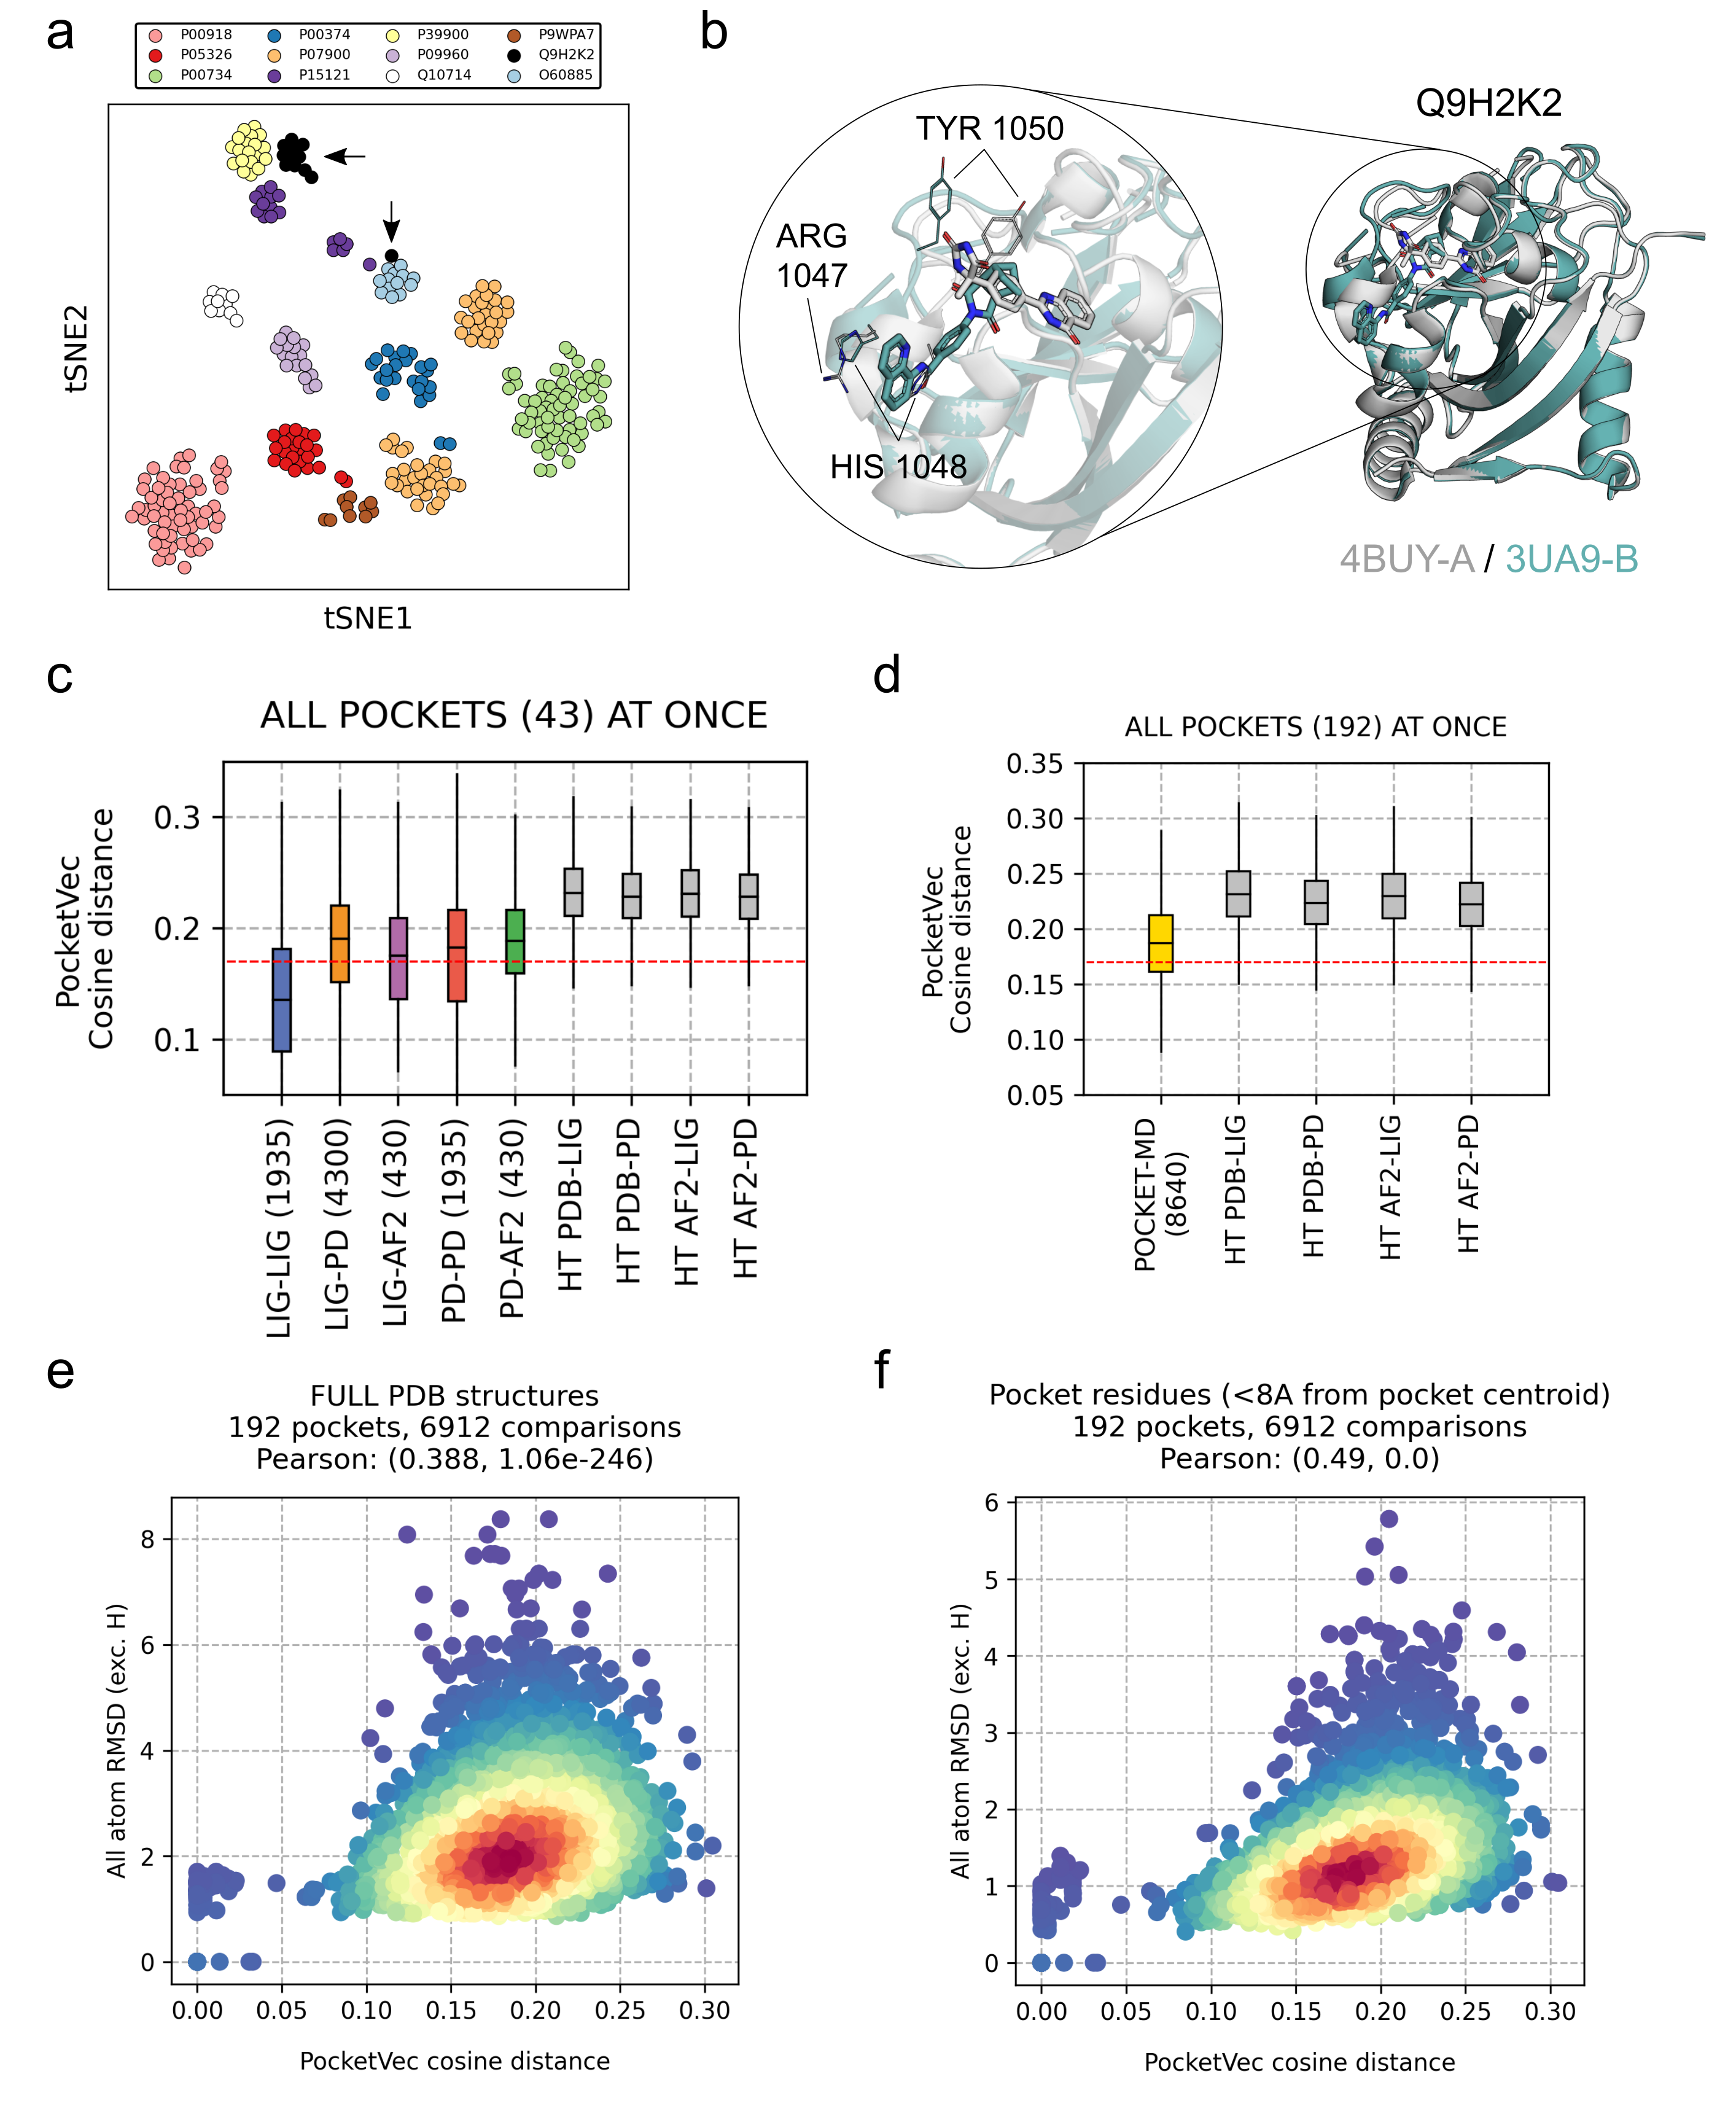
\includegraphics[width=\linewidth]{figures/PocketVec/Main/Fig4.png} 
  \caption{
    \textbf{Assessment of the effect of protein flexibility.} 
    \textbf{a)} 2D tSNE representation of 326 PocketVec descriptors representing the conformational ensemble of 12 pockets binding distinct ligands (ProSPECCTs P1). Black arrows indicate the Poly-ADP polymerase tankyrase-2 (Q9H2K2) structures.
    \textbf{b)} Structural superimposition of 4BUY\_A (white) against 3UA9\_B (teal) performed with TM-align\cite{zhang_tm-align_2005}.
    \textbf{c)} PocketVec descriptors’ variability caused by protein flexibility and conformational changes. Each boxplot indicates the distribution of PocketVec distances of the same pocket in i) holo PDB structures (LIG-LIG), ii) holo and apo PDB structures (LIG-PD), iii) holo PDB and AF2 structures (LIG-AF2), iv) apo PDB structures (PD-PD), v) apo PDB and AF2 structures (PD-AF2) and holo (LIG), apo (PD) and AF2 structures (AF2) against each of the 4 sets of PocketVec descriptors from our study (i.e. PDB-LIG, PDB-PD, AF2-LIG, AF2-PD). Boxplots indicate median (middle line), 25th, 75th percentile (box), and max and min value within the 1.5*25th and 1.5*75th percentile range (whiskers).
    \textbf{d)} PocketVec descriptors’ variability caused by protein flexibility and conformational changes among MD-derived structures. POCKET-MD represents the distances between same-pocket MD-derived PocketVec descriptors and all the other boxplots represent the distances between such MD-derived descriptors and each of the 4 sets already precomputed (i.e. PDB-LIG, PDB-PD, AF2-LIG, AF2-PD).
    \textbf{e)} Correlation between PocketVec cosine distance (x-axis) and all-atom (excluding hydrogens) RMSD for the full PDB structure and
    \textbf{f)} pocket residues only. The study involved 192 pockets (8 from PDB-LIG and 184 from PDB-PD) with MD-simulation data (3 frames per replica, 3 replicas). Both plots are colored by density (the redder the higher).
  }
  \label{PocketVec_Fig4}
\end{figure}


%%%%%%%%%%%%%%%%%%%%%%%%%%%%%%%%%%%%%%%%%%%%%%%%%%%%%%%%%%%%%%%%
%%% All-vs-all comparison of human druggable pockets
%%%%%%%%%%%%%%%%%%%%%%%%%%%%%%%%%%%%%%%%%%%%%%%%%%%%%%%%%%%%%%%%

\phantomsection
\subsubsection{All-vs-all comparison of human druggable pockets}
\label{PocketVec_ResultsAndDiscussion_All_vs_All_comparison_human_druggable_pockets}

The vector-like nature of PocketVec descriptors makes them perfectly suited for extremely fast comparisons by computing simple cosine distances, enabling comprehensive proteome-wide similarity searches. We first generated a t-distributed Stochastic Neighbor Embedding (t-SNE) representation for all PocketVec descriptors to facilitate a qualitative visualization of the characterized pocket space (Fig \ref{PocketVec_Fig3}e). This visualization underlined several interesting points, some of which have already been discussed in previous sections: (i) pockets defined by bound ligands (PDB-LIG and AF2-LIG) predominantly occupy well defined regions of the pocket space, (ii) pocket detection strategies (PDB-PD and AF2-PD) significantly contribute to expand the overall coverage of the human druggable pocket space, (iii) the use of AF2 models particularly bolsters this expansion. Perhaps more interestingly, the PDB-PD and AF2-PD maps highlight dense areas of the human pocket space for which we do not yet have any experimental structure with a bound chemical compound.

Then, we systematically evaluated the validity of the chemogenomic hypothesis behind the generation of PocketVec descriptors (i.e. similar pockets bind similar ligands). We compared all PDB-LIG pockets having PocketVec descriptors (1,594 pockets, \textasciitilde1.27M comparisons) on the basis of the maximum Tanimoto similarity among their bound ligands using ECFPs (2,048 bits and radius 2), and we grouped pocket pairs according to their cosine PocketVec distance (Fig \ref{PocketVec_Fig3}f). We found that, indeed, pocket pairs with small PocketVec distances (<0.10) typically showed higher maximum Tanimoto similarities (>0.85) among their ligands than pocket pairs with high PocketVec distance (>0.17, Fisher’s exact test OR >90 and p-value <10\textsuperscript{-300}), thus supporting our underlying hypothesis. However, the fact that similar pockets bind similar ligands does not necessarily imply that similar ligands bind similar pockets. Indeed, we observed that, in general, PocketVec distances did not decrease substantially when increasing the maximum Tanimoto similarity among bound ligands (Fig \ref{PocketVec_Fig3}g). The only exception was for almost identical ligands (Tanimoto similarities=1), which showed a very subtle deviation towards smaller PocketVec distances (AUROC 0.59, true positives having Max. Tanimoto Similarity=1, true negatives having Max. Tanimoto Similarity in the [0, 0.5) range), in line with the behavior observed in ProSPECCTs P5 (AUROC=0.64) and P5.2 (AUROC=0.62). While this may seem somewhat counterintuitive, it serves as evidence to decipher the quantification of pocket similarity using PocketVec descriptors. 

The fact that a single compound is consistently upranked for two pockets may indeed be a first evidence of pocket similarity but falls short to provide similar PocketVec descriptors if no other compound is ranked in a systematic manner. In practical terms, this translates into pockets that share a growing number of ligands being more likely to be similar from a PocketVec perspective, as highlighted by Shoichet and co-workers when they presented their similarity ensemble approach (SEA) to unveil protein remote relationships\cite{keiser_relating_2007}. Reassuringly, we found that pockets that shared ligands in the PDB-LIG set tended to be more similar (i.e. smaller PocketVec distances) than pockets sharing no ligands (Fig \ref{PocketVec_Fig3}h). However, the deviation towards smaller distances for pockets sharing a single ligand was subtle (AUROC = 0.58, true positives sharing 1 ligand and true negatives sharing no ligands), but when 3 or more ligands were shared between pockets, the effect was already notable (AUROC = 0.75, true positives sharing 3 or more ligands and true negatives sharing no ligands). We also found that only 2.1\% of pocket pairs sharing no ligands in the PDB-LIG set showed PocketVec distances <0.17, while this fraction increased to 26.1\% when 3 or more ligands were shared between pockets. However, it is obvious that the lack of shared co-crystallized compounds between two pockets does not necessarily mean that they might not have common ligands. To overcome the limitation of potentially missing ligands, we used a pure computational strategy: we computed docking scores for the 128 standard lead-like molecules (see \hyperref[PocketVec_MethDevAndImp]{Methodological development and implementation}) against all PDB-LIG defined pockets and labeled them as active (the top 1\% of docking scores) or inactive (Fig \ref{PocketVec_FigS26}a). We observed that the vast majority of the lead-like molecules (127 out of 128) were cataloged as active in, at least, one pocket (Fig \ref{PocketVec_FigS26}b), and almost 20,000 of the potential \textasciitilde1,29M PDB-LIG pocket pairs shared, at least, one active lead-like molecule (Fig \ref{PocketVec_FigS26}c). With this alternative approach, we confirmed the tendency observed using experimental data: the more shared ligands between pockets, the smaller their PocketVec distance (AUROC = 0.87 when comparing pockets sharing no ligands and those sharing 3 or more ligands; Fig \ref{PocketVec_FigS26}d).

Next, we explored the complementarity and added value of PocketVec descriptors with respect to more established strategies to compare protein families and druggable pockets, such as sequence and structure similarity. First, we sought to investigate the correlation between sequence, structure and PocketVec similarity (defined as 1-PocketVec distance) among pockets located in the same Pfam domains in the more comprehensive set of AF2-PD pockets (see \hyperref[PocketVec_Methods]{Methods}). As expected, we found that the higher the sequential and structural similarity between compared pockets (assessed by sequence identity and C$\alpha$ RMSD, respectively), the more similar they were according to PocketVec descriptors (Pearson CC of 0.55 and -0.35, respectively, p-value<10\textsuperscript{-100} in both cases; Fig \ref{PocketVec_Fig5}a). Reassuringly, the observed correlations were also found when computed on AF2-LIG pockets (Pearson CC of 0.57 and -0.35 for sequence identity and C$\alpha$ RMSD, respectively Fig \ref{PocketVec_FigS27}). However, there were indeed cases where the results did not align perfectly, underscoring the distinctive and complementary insights that PocketVec descriptors can provide beyond traditional sequential and structural analyses.

Additionally, we also ran an all-against-all pocket comparison within and across pocket sets (PDB-LIG, PDB-PD, AF2-LIG and AF2-PD), computing over 1.2 billion pocket comparisons. Interestingly, we found more than 3.5 million similar pockets in domains having low sequential and structural similarities (PocketVec distance <0.17; TM-score <0.35; Sequence identity <30\%). For instance, we found similar pockets (PocketVec distance: 0.14, both pockets in the PDB-LIG set) in the CPSase\_L\_D2 ATP-binding domain (PF02786) of the Carbamoyl-phosphate synthase (P31327, positions 1088-1291) and in the NDK domain of the Nucleoside diphosphate kinase 3 (Q13232, positions 22-156), although they shared a sequence identity of only 28\% and a poor structural similarity (TM-score=0.31, RMSD=4.3Å). Reassuringly, crystal structures confirmed that both pockets can bind ADP (PDB IDs: 5DOU and 1ZS6, respectively), which strengthened our observation that these pockets were indeed similar (Fig \ref{PocketVec_Fig5}b). The inventory of all similar pockets (PocketVec distance <0.17) together with structural and sequential comparisons at domain level are reported in our \hl{GitLab}. On the other hand, our analyses also revealed more than 29k pocket pairs (out of a subsample of 11.1 million pairs having PocketVec distance >0.20) that, despite being similar in terms of sequence and structure, showed quite dissimilar pockets (PocketVec distance >0.20; TM-score >0.50; Sequence identity >40\%). As an illustrative example, we identified different druggable pockets (PocketVec distance: 0.21, both pockets in the AF2-PD set) in the NIPSNAP domain (PF07978) of the Protein NipSnap homolog 3B (Q9BS92, positions 146-245) and in the NIPSNAP domain (PF07978) of the Protein NipSnap homolog 3A (Q9UFN0, positions 146-245), although these domains had a sequence identity of 93\% and also a very high level of structural similarity (Fig \ref{PocketVec_Fig5}c, TM-score=0.98 and RMSD=0.4Å).

%%%%%%%%%%%%%%%%
%%% FIGURE 5 %%%
%%%%%%%%%%%%%%%%

\begin{figure}[H]
  \centering
  \includegraphics[width=\linewidth]{figures/PocketVec/Main/Fig5.png} 
  \caption{
    \textbf{Using PocketVec descriptors to assess proteome-wide pocket similarity: achieving otherwise unattainable insights.} 
    \textbf{a)} Correlation between PocketVec similarity (x-axis, defined as 1-PocketVec distance), structural similarity (y-axis, C$\alpha$ RMSD) and sequence identity (color) among pockets located at the same Pfam domains (max. 10) in the AF2-PD pocket set. Pearson CC between PocketVec similarity and sequence identity: 0.55 (p-value\textasciitilde0). Pearson CC between PocketVec similarity and RMSD: -0.35 (p-value\textasciitilde0).
    \textbf{b)} Similar pockets found in dissimilar domains. Pockets were found in the CPSase\_L\_D2 ATP-binding domain (PF02786, top structure, wheat color) of the Carbamoyl-phosphate synthase (P31327, positions 1088-1291. PDB ID: 5DOU) and in the NDK domain (PF00334, bottom structure, pale green color) of the Nucleoside diphosphate kinase 3 (Q13232, positions 22-156. PDB ID: 1ZS6). Pockets (both in the PDB-LIG set) have a PocketVec distance of 0.14 (below the established threshold of 0.17, please see \hyperref[PocketVec_ResultsAndDiscussion_PocketVec_performance_on_the_ProSPECCTs_benchmark]{PocketVec performance on the ProSPECCTs benchmark sets}) although domains share a sequence identity of only 28\% and a poor structural similarity (TM-score=0.31, RMSD=4.3Å).
    \textbf{c)} Dissimilar pockets found in similar domains. Pockets were found in the NIPSNAP domain (PF07978) of the Protein NipSnap homolog 3B (Q9BS92, positions 146-245, AF2 model, pink residues) and in the NIPSNAP domain (PF07978) of the Protein NipSnap homolog 3A (Q9UFN0, positions 146-245, AF2 model, green residues). The former is used as the reference structure (gray cartoon). Pockets (both in the AF2-PD set) have a PocketVec distance of 0.21 (above the established threshold of 0.17, please see \hyperref[PocketVec_ResultsAndDiscussion_PocketVec_performance_on_the_ProSPECCTs_benchmark]{PocketVec performance on the ProSPECCTs benchmark sets}) although domains have a sequence identity of 93\% and also a very high level of structural similarity (TM-score=0.98 and RMSD=0.4Å).
  }
  \label{PocketVec_Fig5}
\end{figure}




%%%%%%%%%%%%%%%%%%%%%%%%%%%%%%%%%%%%%%%%%%%%%%%%%%%%%%%%%%%%%%%%
%%% Relationship between PocketVec similarity and experimentally determined compound-target pairs
%%%%%%%%%%%%%%%%%%%%%%%%%%%%%%%%%%%%%%%%%%%%%%%%%%%%%%%%%%%%%%%%

\phantomsection
\subsubsection{Relationship between PocketVec similarity and experimentally determined compound-target pairs}
\label{PocketVec_ResultsAndDiscussion_Relationship_PocketVecSimilarity_CPD-TARGET_pairs}

To further validate the ability of PocketVec descriptors to identify similar protein binding pockets, we explored the relationship between pocket similarity and experimentally determined compound-target pairs by assessing the number of shared compounds between proteins with different degrees of pocket similarity. We processed data on 836,654 compounds bound to 6,933 protein targets from ChEMBL\cite{zdrazil_chembl_2024} and BindingDB\cite{gilson_bindingdb_2016}, and we also collected all PocketVec descriptors from our study (i.e. PDB-LIG, PDB-PD; AF2-LIG and AF2-PD) and kept only those protein pairs for which there was, at least, one reported bound small molecule per protein (\hyperref[PocketVec_Methods]{Methods}). Overall, we evaluated 2,055,378 protein pairs on the bases of the number of shared compounds and the cosine distances between their PocketVec descriptors. Note that, since the experimental data reported compound-target pairs, without information on specific pockets, we always took the minimal PocketVec distance between each pair of proteins (i.e. the most similar pockets). 

We first calculated the number of protein pairs within each range of PocketVec distances in an all-vs-all comparison of PocketVec descriptors, regardless of their set of origin (e.g. PDB-LIG, AF2-PD, etc) (Fig \ref{PocketVec_Fig6}a). Then, we checked the distribution of shared compounds between each protein pair plotted against their minimal PocketVec distance. We observed that, the lower the minimal PocketVec distance between two proteins, the higher the number of compounds binding them both and, for PocketVec distances ≥0.2, there were almost no shared compounds for any protein pair (Fig \ref{PocketVec_Fig6}b). Further, we calculated the odds ratio considering a varying number of shared compounds for PocketVec distances ≤0.17, ≤0.10 and ≤0.05. We found that, indeed, there was a clear enrichment of protein pairs sharing compounds among protein pairs with similar pockets. (Fig \ref{PocketVec_Fig6}c). For instance, we found \textasciitilde2, \textasciitilde50 and \textasciitilde200 fold enrichments of protein pairs sharing ≥5 compounds in protein pairs with minimal PocketVec cosine distances below 0.17, 0.10 and 0.05, respectively. And these enrichments went up to \textasciitilde5, \textasciitilde300 and \textasciitilde700 if we considered protein pairs sharing ≥20 compounds. Finally, to overcome potential biases due to the comparison of PocketVec descriptors from the same origin (e.g. PDB-LIG, AF2-PD, etc), we repeated the analysis considering only comparisons between the PDB-LIG set (i.e. derived from experimental structures with co-crystallized compounds) and the other sets, observing a very similar result (Fig \ref{PocketVec_FigS28}a, b, c).

Additionally, we checked the robustness of our results on a novel dataset where Winter and co-workers comprehensively tested the potential binding of 407 fragment compounds on 5,951 proteins. After applying the filtering criteria to the raw data defined by the authors, we analyzed 301 fragment compounds and 525 proteins for which we had PocketVec descriptors (\hyperref[PocketVec_Methods]{Methods}). We repeated the analyses described above finding that, despite the much lower number of instances (from \textasciitilde2.1M protein pairs to \textasciitilde140k), protein pairs with similar pockets tended to share more fragments (Fig \ref{PocketVec_Fig6}d, e), which also translated in significant enrichments (Fig \ref{PocketVec_Fig6}f). In this case, we found no enrichment of common compounds for PocketVec distances ≤0.17, which was expected due to the smaller nature of the fragments (translating in lower specificity). However, we observed enrichments of protein pairs sharing ≥3 compounds of \textasciitilde8 and \textasciitilde30 fold for PocketVec distances ≤0.10 and ≤0.05, respectively. For completeness, we also ran the same analyses considering only comparisons between the PDB-LIG and the other PocketVec descriptor sets (Fig \ref{PocketVec_FigS28}d, e, f). However, although we still observed a similar trend, the counts were too low to extract any significant conclusion.

Overall, these new results show that, indeed, there is a clear relationship between pocket similarities, as defined by low PocketVec distances, and the probability of those proteins to experimentally bind the same compounds, further validating our approach.


%%%%%%%%%%%%%%%%
%%% FIGURE 6 %%%
%%%%%%%%%%%%%%%%

\begin{figure}[H]
  \centering
  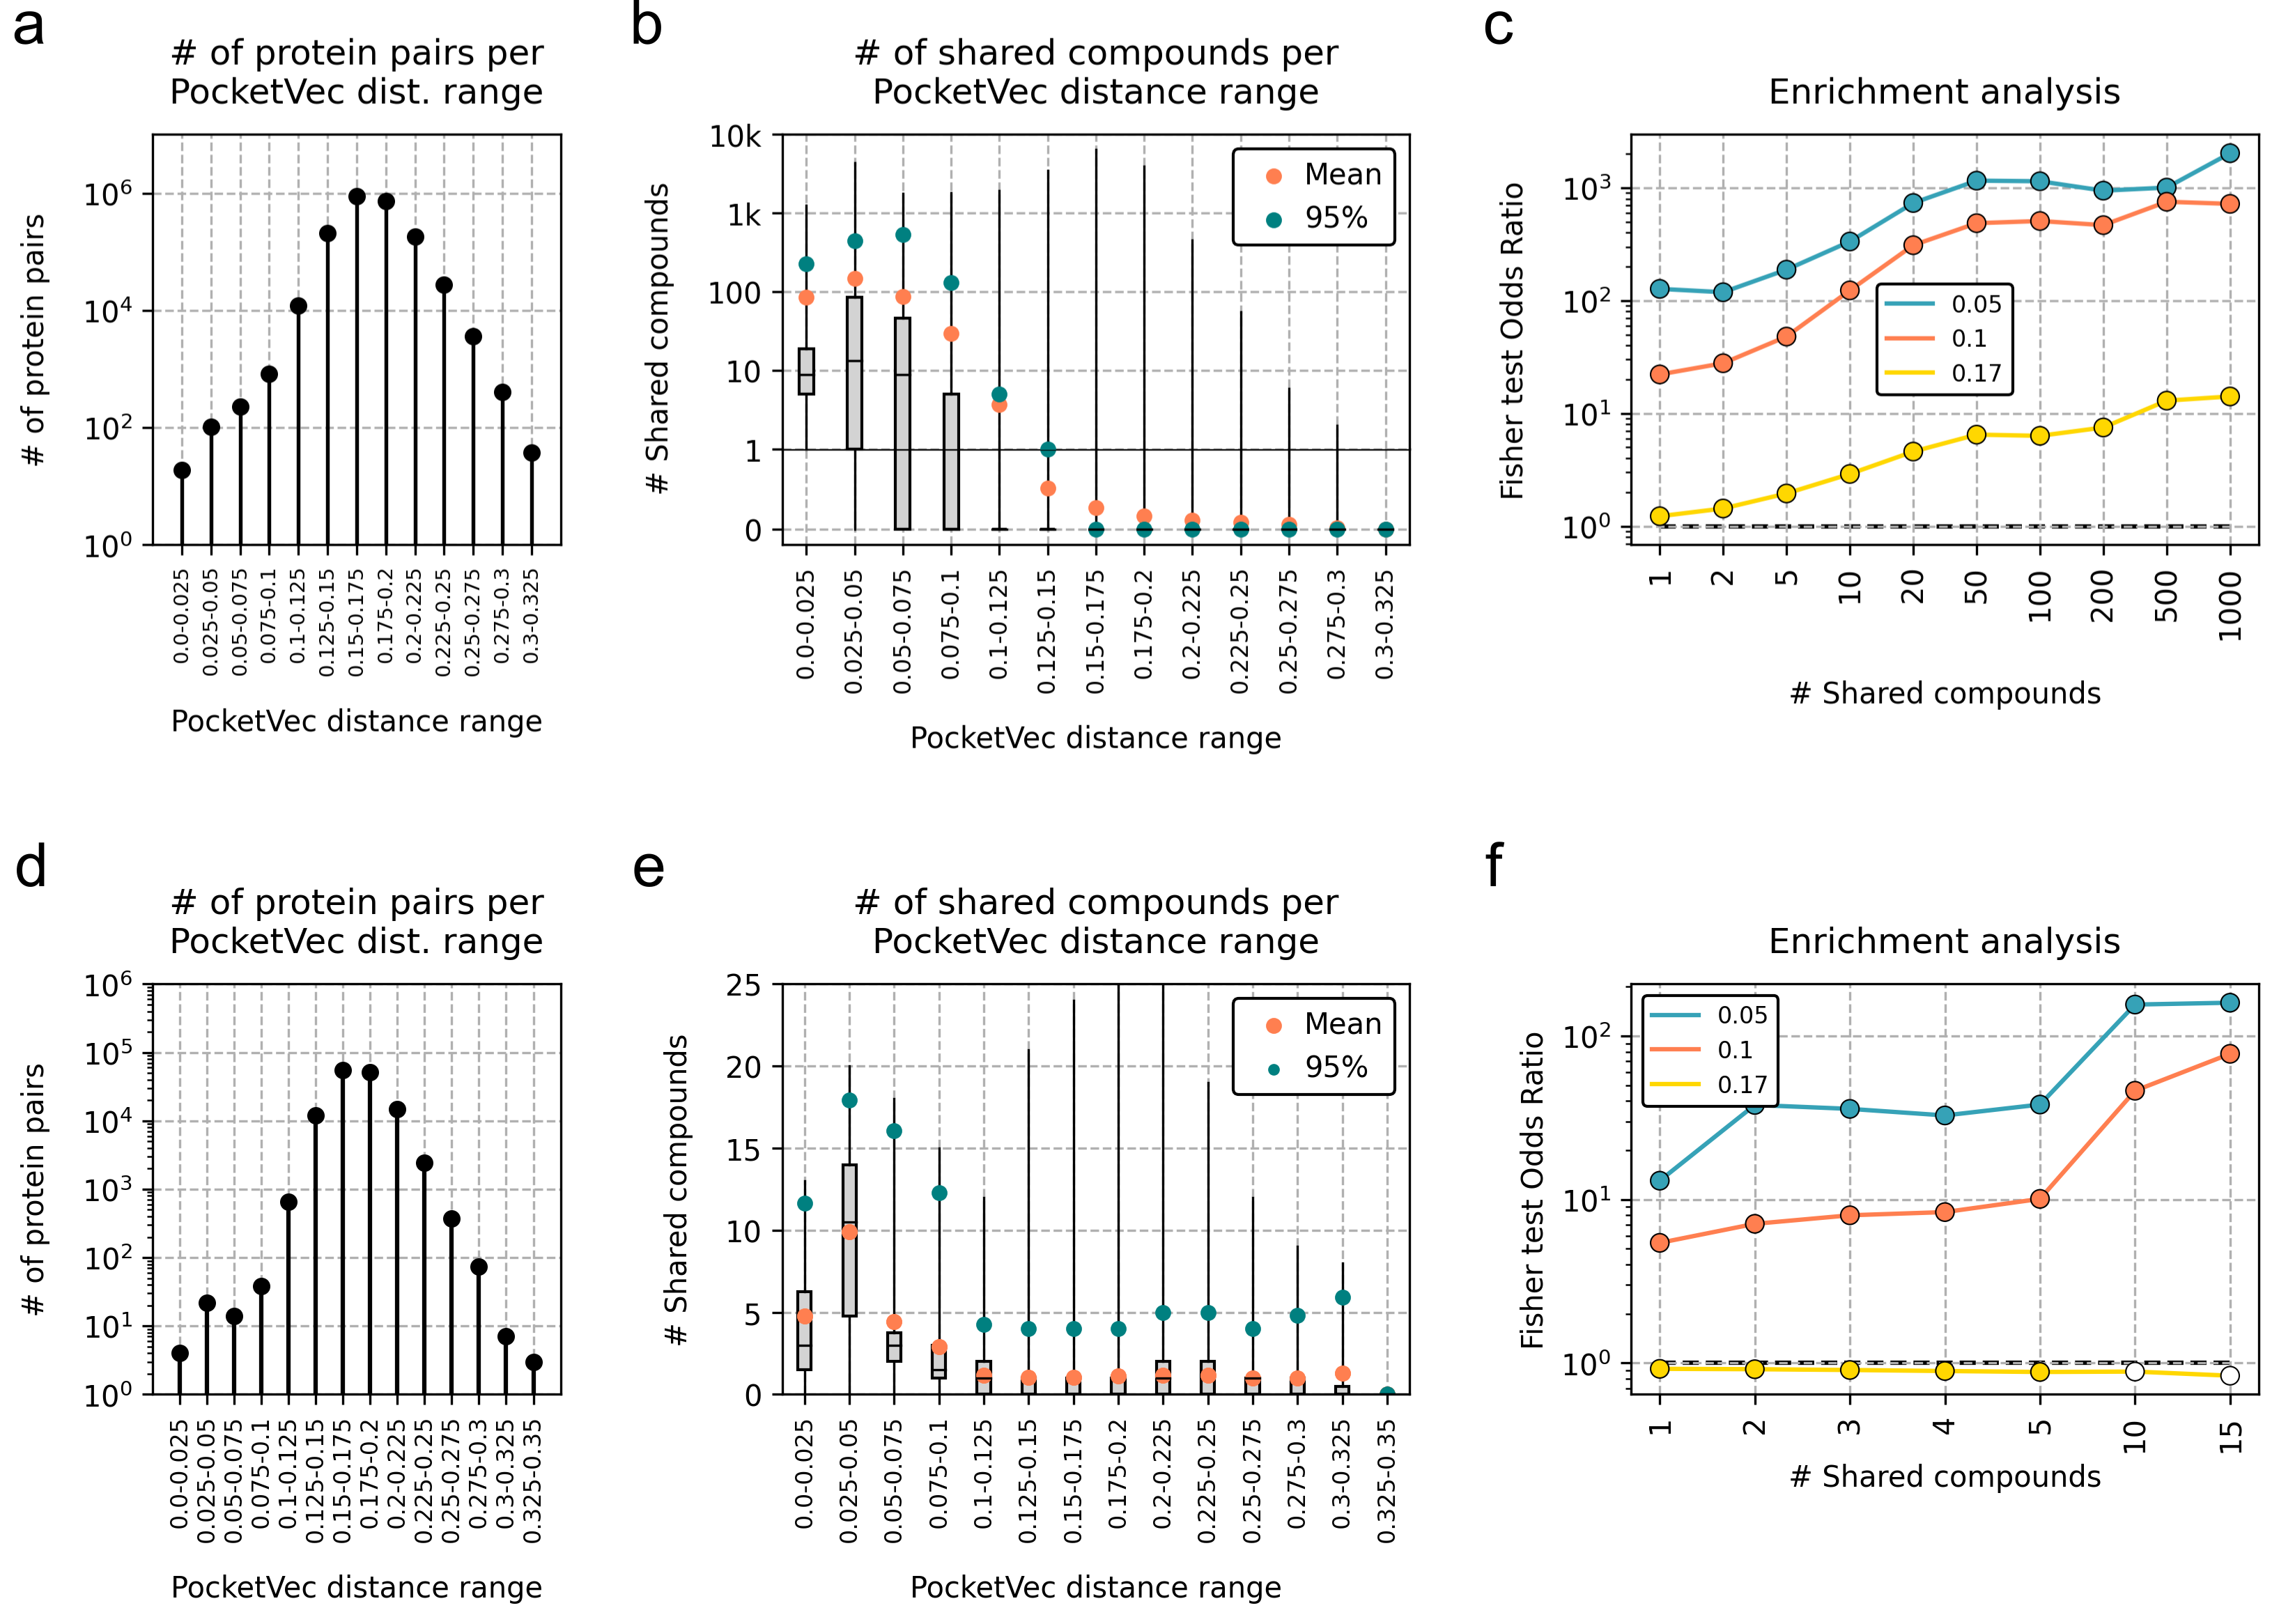
\includegraphics[width=\linewidth]{figures/PocketVec/Main/Fig6.png} 
  \caption{
    \textbf{Relationship between PocketVec similarity and experimentally determined compound-target pairs.}
    All vs All (PDB-LIG, PDB-PD, AF2-LIG and AF2-PD) comparison between PocketVec distance and number of shared compounds among proteins having experimental binding data in ChEMBL and BindingDB (a, b, c) and Offensperger et al.\cite{offensperger_large-scale_2024} (d, e, f).
    \textbf{a, d)} Number of protein pairs (y-axis) at each PocketVec distance range (x-axis).
    \textbf{b, e)} Number of shared compounds for all pairs having a PocketVec distance in the specified distance range. Orange dots indicate the average value while green dots indicate the lower bound for the top 5\% of the pairs. Boxplots indicate median (middle line), 25th, 75th percentile (box), and maximum and minimum values (whiskers). 
    \textbf{c, f)} Evolution of Fisher test Odds Ratio (y-axis) for an increasing number of shared compounds (x-axis) using an increasing value of PocketVec distance cut-off (0.05, 0.10 and 0.17). Colored dots indicate pvalue <0.001, gray dots indicate pvalue <0.05 and white dots indicate pvalue >0.05.
  }
  \label{PocketVec_Fig6}
\end{figure}

%%%%%%%%%%%%%%%%%%%%%%%%%%%%%%%%%%%%%%%%%%%%%%%%%%%%%%%%%%%%%%%%
%%% Identifying kinases with similar inhibition profiles through PocketVec descriptors
%%%%%%%%%%%%%%%%%%%%%%%%%%%%%%%%%%%%%%%%%%%%%%%%%%%%%%%%%%%%%%%%

\phantomsection
\subsubsection{Identifying kinases with similar inhibition profiles through PocketVec descriptors}
\label{PocketVec_ResultsAndDiscussion_Identifying_Kinases}


Bla bla bla



\subsection{Concluding remarks}

We have presented PocketVec, a novel approach to generate vector-like protein pocket descriptors based on inverse docking and the chemogenomics principle that similar pockets bind similar ligands. A thorough assessment of its performance ranks it among the best available methodologies to characterize and compare protein druggable pockets, while overcoming some important limitations. We have also systematically searched for druggable pockets in the folded human proteome, using experimentally determined protein structures and AF2 models, identifying over 32,000 binding sites in more than 20,000 protein domains. We then derived PocketVec descriptors for each small molecule binding site and took advantage of their vector-like format to run an all-against-all pocket similarity search, exploring over 1.2 billion pairwise comparisons. Besides, we provide pre-computed descriptors for every identified human pocket together with the annotated Python code to generate new descriptors for any pocket of interest. We found that PocketVec descriptors are complementary to other, more classical, search strategies, enabling the identification of pocket similarities not revealed by structure- or sequence-based comparisons. As illustrative examples of applicability, we unveiled a clear relationship between pocket similarities, as defined by low PocketVec distances, and the probability of those pockets to bind the same compounds, as experimentally detected. Moreover, a systematic comparison of druggable pockets in protein kinases showed that kinase pairs with similar PocketVec descriptors also exhibited similar experimentally determined inhibition profiles. 

There have been recent attempts to identify druggable pockets at the proteome level\cite{wang_cavityspace_2022, konc_probis-fold_2022, sim_hproteome-bsite_2022, tsuchiya_possum_2023}. However, the novelty of our ligand-centric methodological approach, the accuracy of our descriptors and the systematic and exhaustive identification and characterization of binding pockets enabled the analyses of the effects of protein structural variation on pocket definition and small molecule binding at an unprecedented scale. Besides, the comprehensive list of human-derived pocket descriptors will become a valuable resource for the bio and cheminformatics communities.

This first generation of descriptors has been primarily designed for global analyses, such as the comprehensive characterization of all human druggable pockets. Indeed, our analyses have revealed dense clusters of similar pockets in distinct proteins for which no inhibitor has yet been co-crystalized, opening the door to strategies to prioritize the development of chemical probes to cover the druggable space\cite{carter_target_2019}. Moreover, our initial descriptors can be easily adapted to cater to specific tasks (i.e. exploring substrate specificity in a given protein family) by refining the selection of predefined lead-like molecules used or fine-tuning the similarity cutoff, thereby enhancing their performance. Of special interest are the anticipation of undesired off-targets as well as the guidance of rational polypharmacology, where single univalent molecules could be designed to target two proteins simultaneously, provided that their druggable pockets are similar enough\cite{duran-frigola_detecting_2017}. However, the main impact is likely to come from proteochemometric approaches, where a combination of ligand and target descriptors are used to train machine learning models\cite{fernandez-torras_connecting_2022}. It has been shown that structure-based descriptors of the targets are often superior to distinguish drug selectivity, although the sequence-based ones are often used when key protein structural details are lacking\cite{bongers_proteochemometrics_2019}. The generation of accurate descriptors derived for not yet described pockets in AF2 protein models overpasses this limitation, and opens up many possibilities. We envisage a scenario where small molecule and pocket descriptors combined are used to train AI-based generative models (e.g. to design new chemical entities that bind each protein druggable cavity\cite{jin_hierarchical_2020, blaschke_reinvent_2020}). Indeed, the estimated space of 10\textsuperscript{33} synthetically accessible drug-like molecules is mostly unexplored and represents a reservoir of potentially bioactive compounds\cite{polishchuk_estimation_2013}. Deep learning strategies have successfully designed new antibiotic scaffolds\cite{wong_discovery_2024} and placed 15 AI-designed drugs in clinical trials, including first-in-class molecules against several targets\cite{jayatunga_ai_2022}. Overall, accurate descriptors of druggable pockets might serve as a cornerstone for the development of generative AI approaches in drug discovery, offering unprecedented opportunities to expedite the design of a chemical toolbox to probe biology and, ultimately, to new therapeutics.
\subsection{Code and data availability}
\label{PocketVec_Code}


Bla bla bla


\subsection{Methods}
\label{PocketVec_Methods}


Bla bla bla


\newpage
\chapter{Discussion}
\label{discussion}

Discussion
\chapter{Concluding remarks}
\label{concluding}
\clearpage

In the coming years, we anticipate a computational chemistry and biology landscape where drug candidates and biological entities will be primarily described by numerical vectors, leveraging available data from both public repositories and in-house experiments. These data would include structural features of the molecules and the targets, together with omics profiles, such as gene expression data, as well as large-scale biological networks and ontologies. Data would be linked at different levels with relatively simple operations, allowing for ultra-large, unbiased and systematic identification of the existing connections between the chemical space and the intricate biological space defined by disease biology. 

Indeed, the significant improvement of both chemical and protein descriptors has prompted the development of proteochemometric strategies, where machine learning models are trained on a combination of ligand and target representations \cite{bongers_proteochemometrics_2019}. These kinds of approaches have already shown superior performances in multi-target bioactivity prediction compared with classical methods \cite{torng_graph_2019}, although some results may be over-optimistic due to biases in the training datasets \cite{chen_hidden_2019}. Moreover, it has been shown that structure-based descriptors are often superior when a detailed definition of the target is needed (e.g. to distinguish drug selectivity among members of the same protein family), while sequence-based ones are better suited for more generic models, especially when key structural details are lacking \cite{bongers_proteochemometrics_2019}.

Only a subset of the approximate 20k canonical proteins that constitute the human proteome possess a binding site amenable to targeting (i.e. binding) by small molecules. Additionally, not all targetable proteins are necessarily disease-modifying, highlighting the need to carefully assess the pharmacological relevance of potential targets. In light of the limitations of small molecules in targeting certain proteins, alternative strategies have emerged to overcome them. For instance, peptides and antibodies often provide higher specificity and affinity than small molecules, particularly when targeting shallow or flat protein surfaces (e.g. protein-protein interaction surfaces). Other approaches involve proximity induced events, such as the use of molecular glues and PROTACs, in which the cellular machinery is hijacked to trigger protein degradation. On a different note, covalent inhibitors can target proteins, including intrinsically disordered proteins, by forming irreversible chemical bonds, leading to sustained inhibition. Together, these diverse strategies offer complementary avenues for expanding the scope and reach of drug discovery efforts. 

However, in view of the enormous complexity inherent to living organisms, as evidenced by the massive amount of bioactivity data gathered and released over the past decades, it is becoming increasingly necessary to move beyond the traditional “one disease-one target-one drug” rationale. Biological systems are highly interconnected, with multiple layers of organization and regulatory networks that contribute to their robustness and adaptability. A more holistic and global view is thus required to bridge translational gaps and accelerate drug discovery efforts to address complex and multifactorial human pathologies.

This thesis represents a very modest contribution in the ever-growing fields of cheminformatics and bioinformatics, encompassed within the wider and long-term process of drug discovery. We hope to add our tiny part and spur future computational efforts along these research lines.


\chapter{Contributions}
\label{Contributions}
\clearpage

As stated in the Objectives section, this thesis aims to explore and further extend the concept of small molecule and protein druggable binding site descriptors, thus laying at the intersection between Cheminformatics and Bioinformatics. Accordingly and, outlined per each chapter, we have made the following contributions:

\begin{enumerate}

\item \textbf{Chapter 3.1}: The implementation of the (preexisting) CC data integration protocol, which represents an optimal framework for generating new bioactivity spaces based on user-provided data, to build novel transcriptomics, proteomics, antibiotics and MoA-based bioactivity signatures. 

\item \textbf{Chapter 3.2}: The use of chemical and bioactivity CC signatures to cluster, visualize and navigate the chemical space of small molecules. In addition, the illustration of the potential of bioactivity signatures to perform such tasks in a biologically relevant manner.  

\item \textbf{Chapter 3.3}: The quantification of bioactivity differences, in terms of protein-ligand binding, between different stereoisomers and the development of stereochemically-aware bioactivity signaturizers. 

\item \textbf{Chapter 3.4}: The development of a novel strategy, named PocketVec, to represent and characterize protein druggable binding sites in the shape of numerical vectors (descriptors). PocketVec descriptors have been comprehensively benchmarked, showing excellent performances in multiple tasks while overcoming the main limitations of existing methods. Additionally, PocketVec descriptors have been generated for all pockets included within human protein domains (using experimentally-determined and accurately-predicted protein structures) and have been proven useful to provide complementary insights to classical structure- and sequence-based comparisons as well as to identify experimentally observed protein similarities in terms of protein-compound binding. 

\end{enumerate}

\thispagestyle{plain}
% \singlespacing
\newpage
% dedication text

\newpage
\vspace*{2cm}

\begin{center}
    ``Has volgut tornar per doblar l'aposta. \\
    Has mirat rient els ulls de la mort. \\
    I arribant a la darrera derrota \\
    has cridat i entès les normes del joc.'' \\
    \vspace{0.3cm}
    -- El gronxador, \textsc{La Ludwig Band}
\end{center}



% the back matter
\clearpage
% \renewcommand*{\bibfont}{\tiny}
% Si es ralla, posar aquesta linia just despres de begin document
\addcontentsline{toc}{chapter}{References}
\bibliography{references}

\begin{appendices}
    % Redefine section to suppress numbering and make it bigger and bold
\titleformat{\section}[block]
  {\normalfont\LARGE\bfseries}{\thesection}{1em}{}
\titlespacing*{\section}{0pt}{*3}{*4}


\chapter{Supplementary Information}
\newpage

\section{Chapter 3.1 -- Navigation}
\section{Chapter 3.2 -- Protocols}
\section{Chapter 3.3 -- Stereoisomers}


\section{Chapter 3.4 -- Comprehensive detection and characterization of human druggable pockets through novel binding site descriptors}

% \renewcommand{\thefigure}{A.\arabic{section}.\arabic{figure}hhh}
\counterwithin{figure}{section}
\setcounter{section}{4} % Assuming section A.4 corresponds to section 4
\setcounter{figure}{0}  % Reset figure counter for this section

% Set caption justification to justified
\captionsetup{justification=justified}
\captionsetup{skip=15pt}

%%%%%%%%%%%%%%%%%%%%
%%% MAIN FIGURES %%%
%%%%%%%%%%%%%%%%%%%%

%%%%%%%%%%%%%%%%%%%%
%% SUPPLEMENTARY %%%
%%%%%%%%%%%%%%%%%%%%

\begin{figure}[htbp]
  \centering
  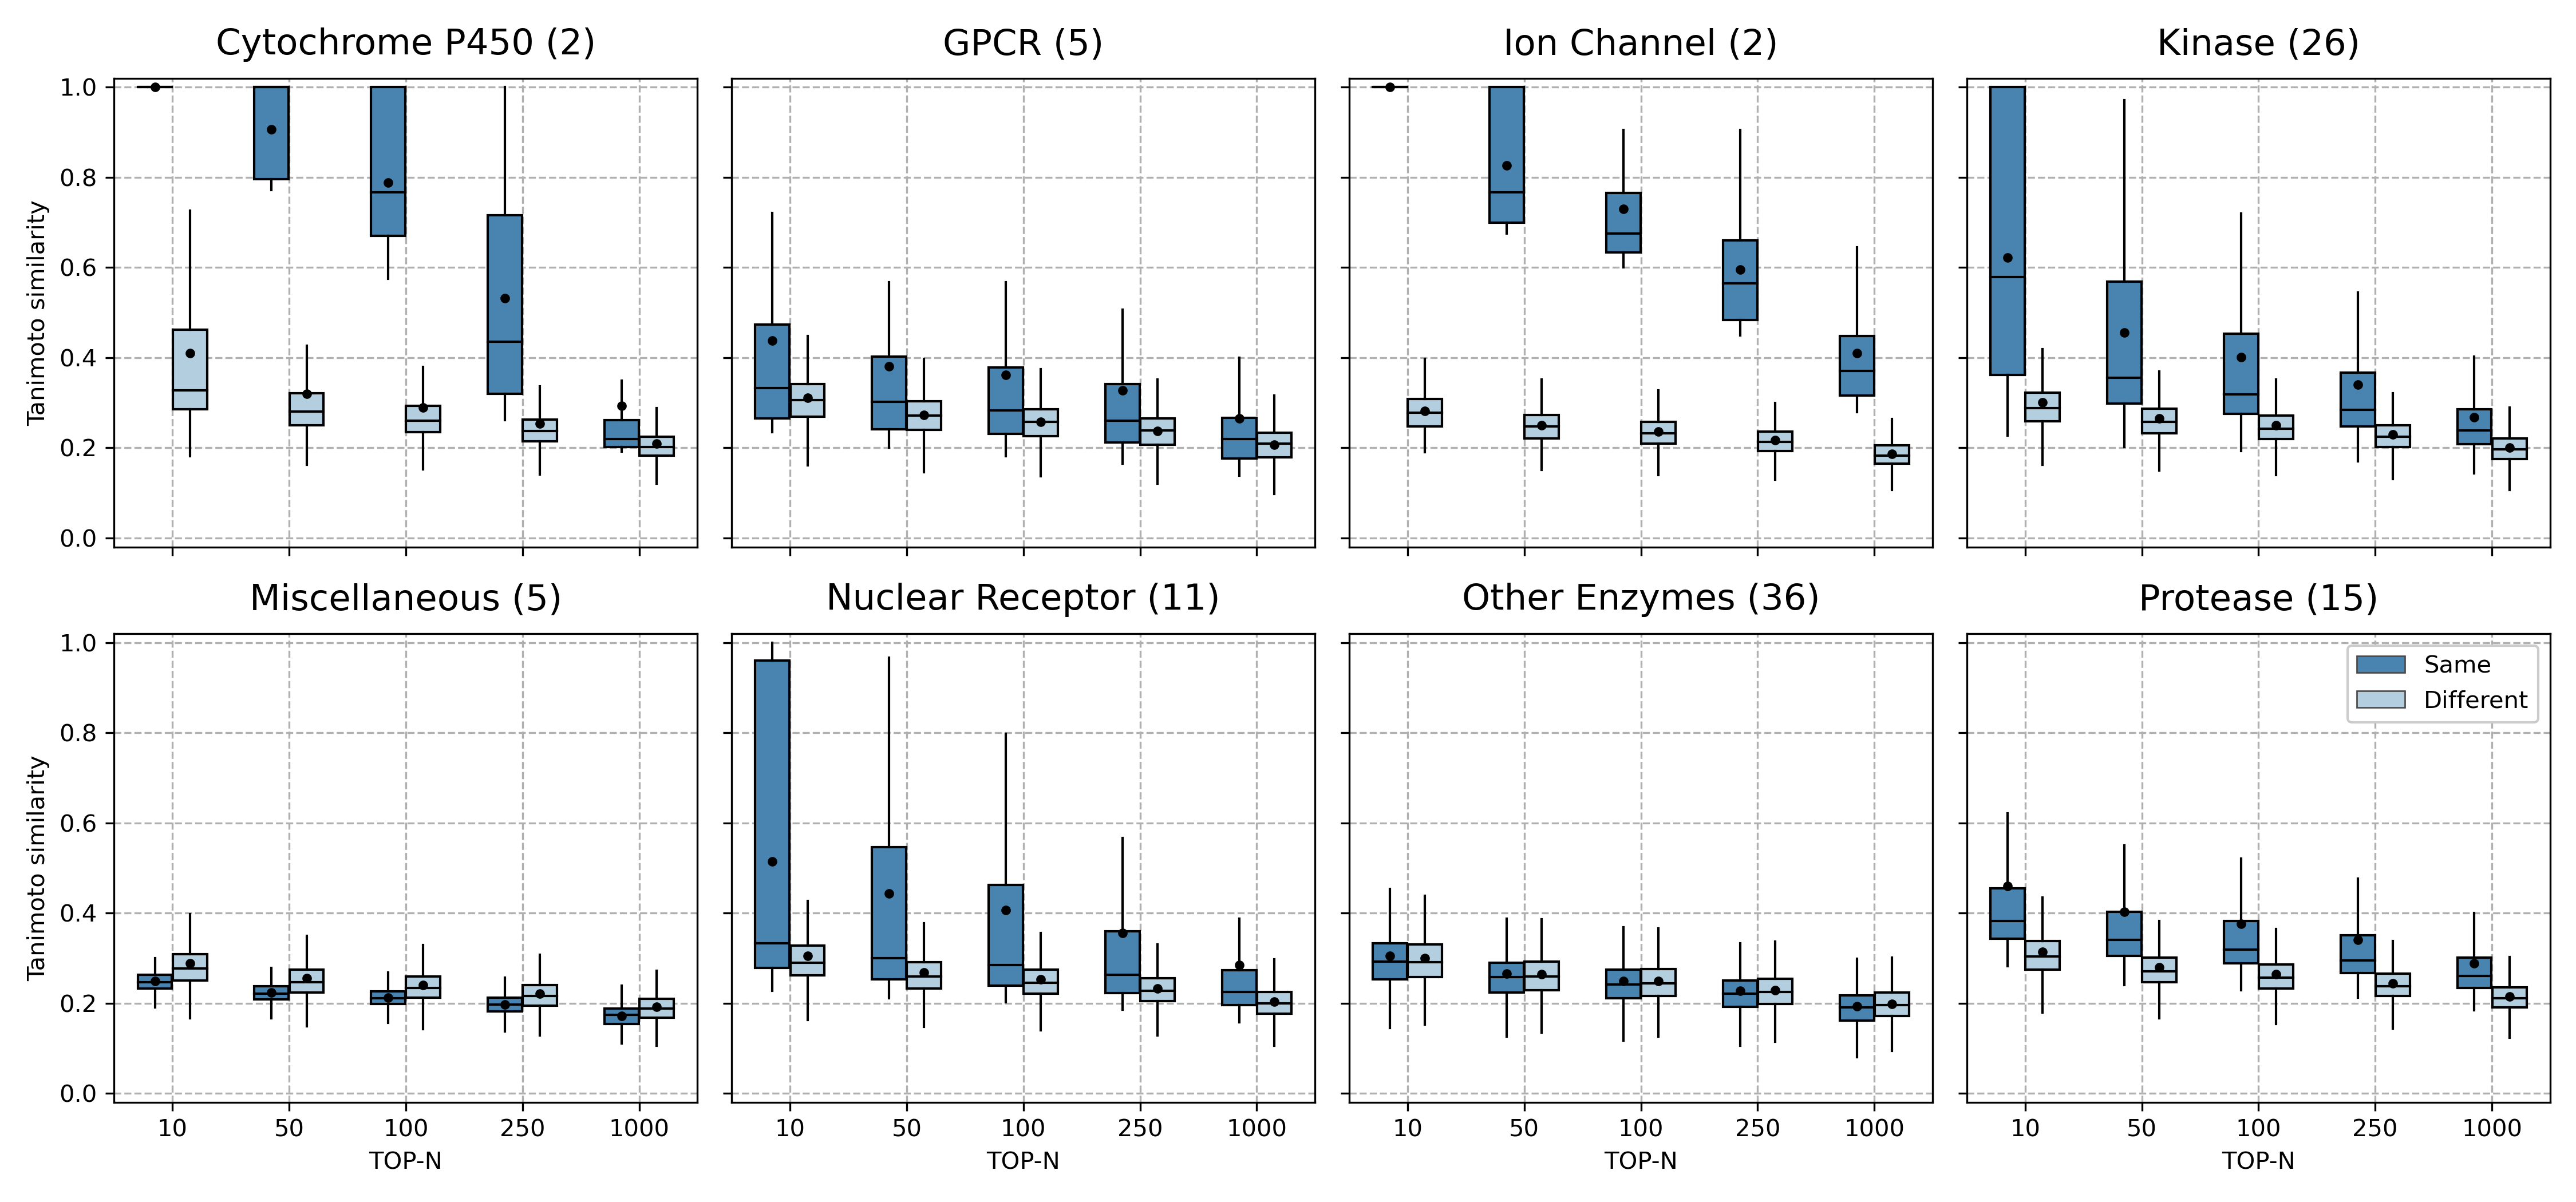
\includegraphics[width=\linewidth]{figures/PocketVec/Supplementary/FigS1.png}
  \caption{Similar proteins bind similar active compounds. For each protein family (e.g. Cytochrome P450, GPCR, etc.) we compared all active compounds between protein pairs from the same family (Same) and from different families (Different). Compounds were compared on the basis of their Tanimoto Similarities (y-axis, ECFP4 with 2048 bits using RDKit – https://rdkit.org) and only the TOP-N (x-axis: 10, 50, 100, 250, 1000) highest similarities were considered per each family. All distributions of Same and Different categories are significantly different (Mann-Whitney U test, pvalue <0.05, alternative greater using SciPy\cite{virtanen_scipy_2020}) except Miscellaneous (10, 50, 100, 250, 1000) and Other Enzymes (10, 50, 100, 250, 1000). Box plots indicate median (middle line), 25th, 75th percentile (box), and max and min value within the 1.5*25th and 1.5*75th percentile range (whiskers). Black dots represent mean values. The number of proteins within each family is specified in the title in parenthesis. Data was downloaded from \href{http://dude.docking.org}{http://dude.docking.org} in January 2023.}
  \label{PocketVec_FigS1}
\end{figure}


\begin{figure}[htbp]
  \centering
  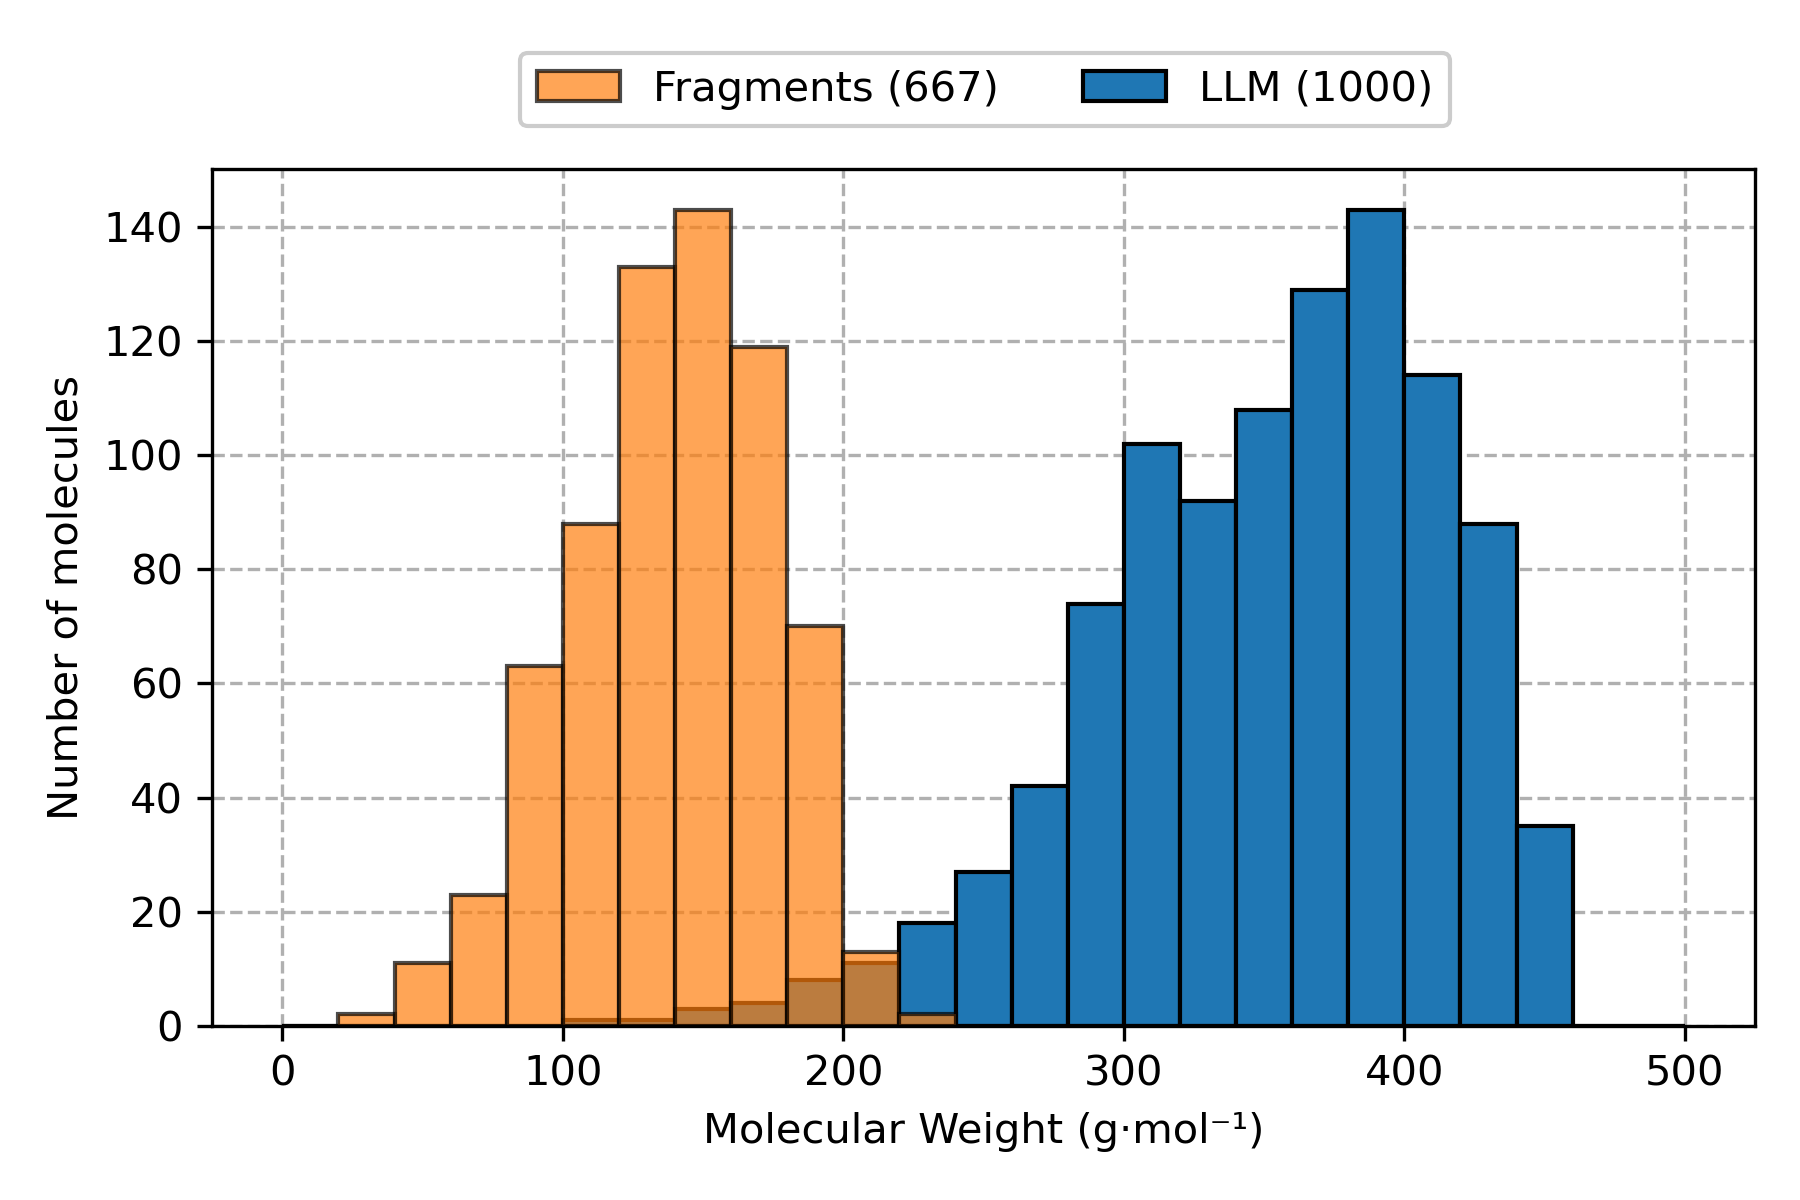
\includegraphics[width=0.65\linewidth]{figures/PocketVec/Supplementary/FigS2.png}
  \caption{
  Histograms of molecular weights (x-axis) from fragments (667, orange) and lead-like molecules (1,000, blue).
  }
  \label{PocketVec_FigS2}
\end{figure}


\begin{figure}[htbp]
  \centering
  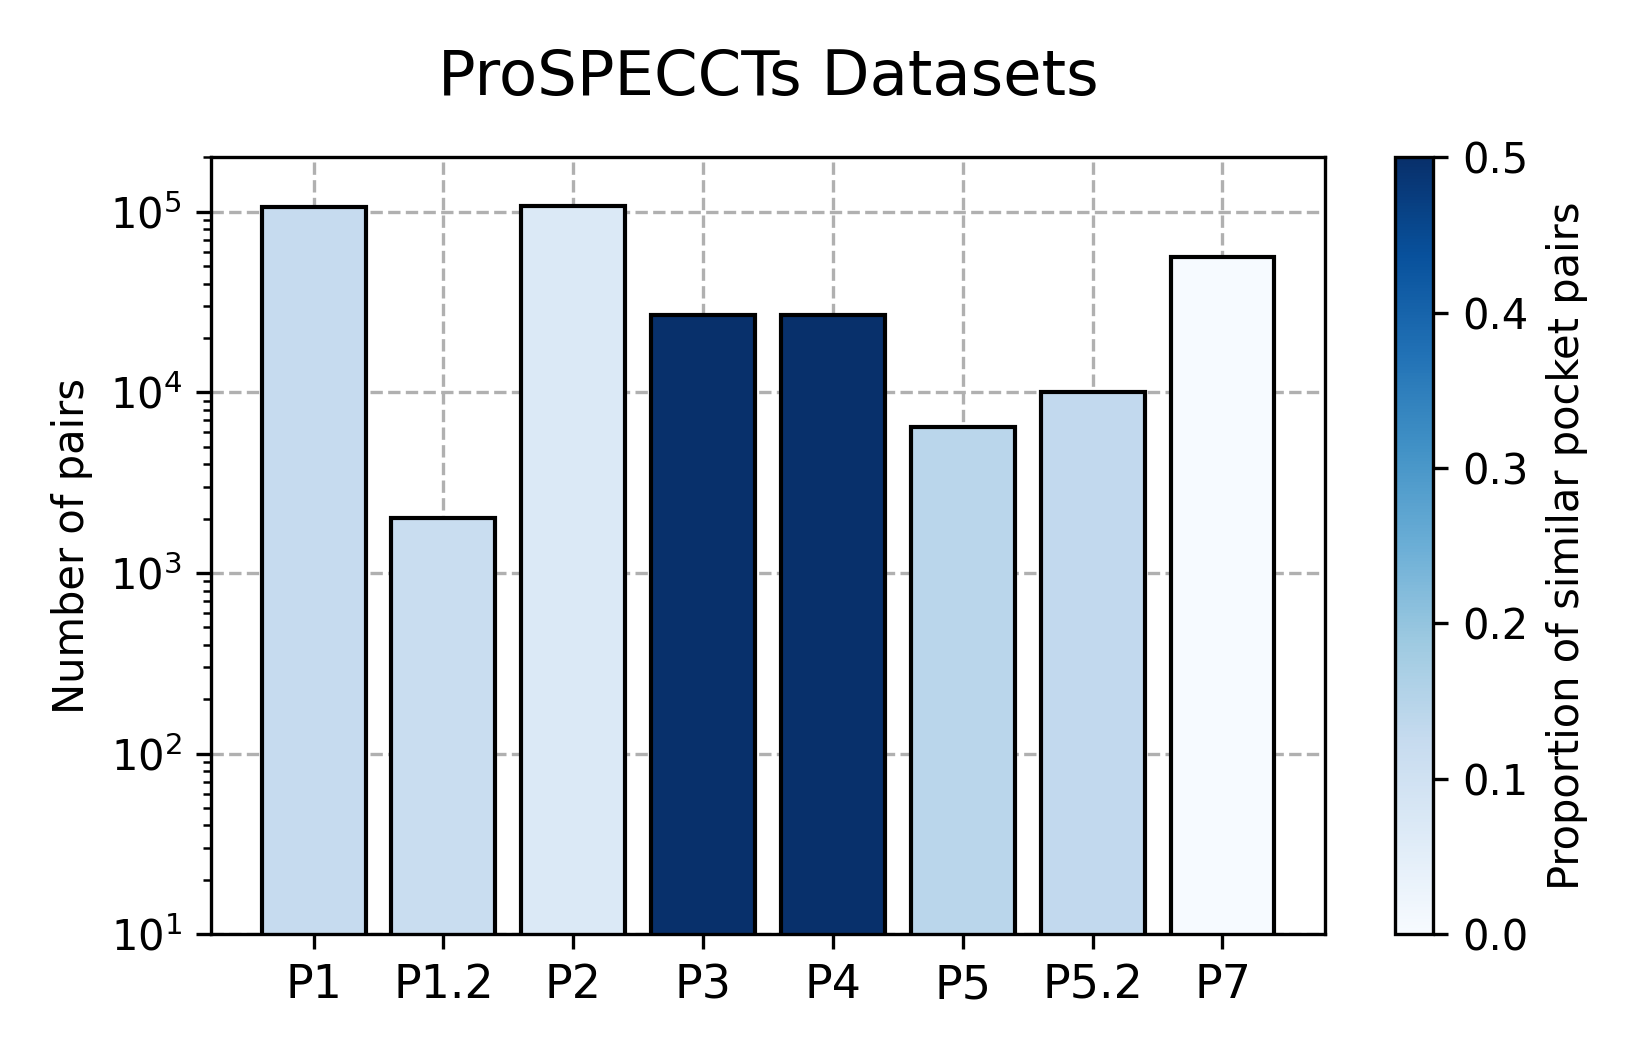
\includegraphics[width=0.75\linewidth]{figures/PocketVec/Supplementary/FigS3.png}
  \caption{
  ProSPECCTs overview. Each bar represents a ProSPECCT dataset (x-axis) and indicates the number of protein-ligand binding site pairs (y-axis) together with the proportion of similar pocket pairs within each dataset (color tone). Please, see the Online Methods section for a detailed description of each dataset.
  }
  \label{PocketVec_FigS3}
\end{figure}


\begin{figure}[htbp]
  \centering
  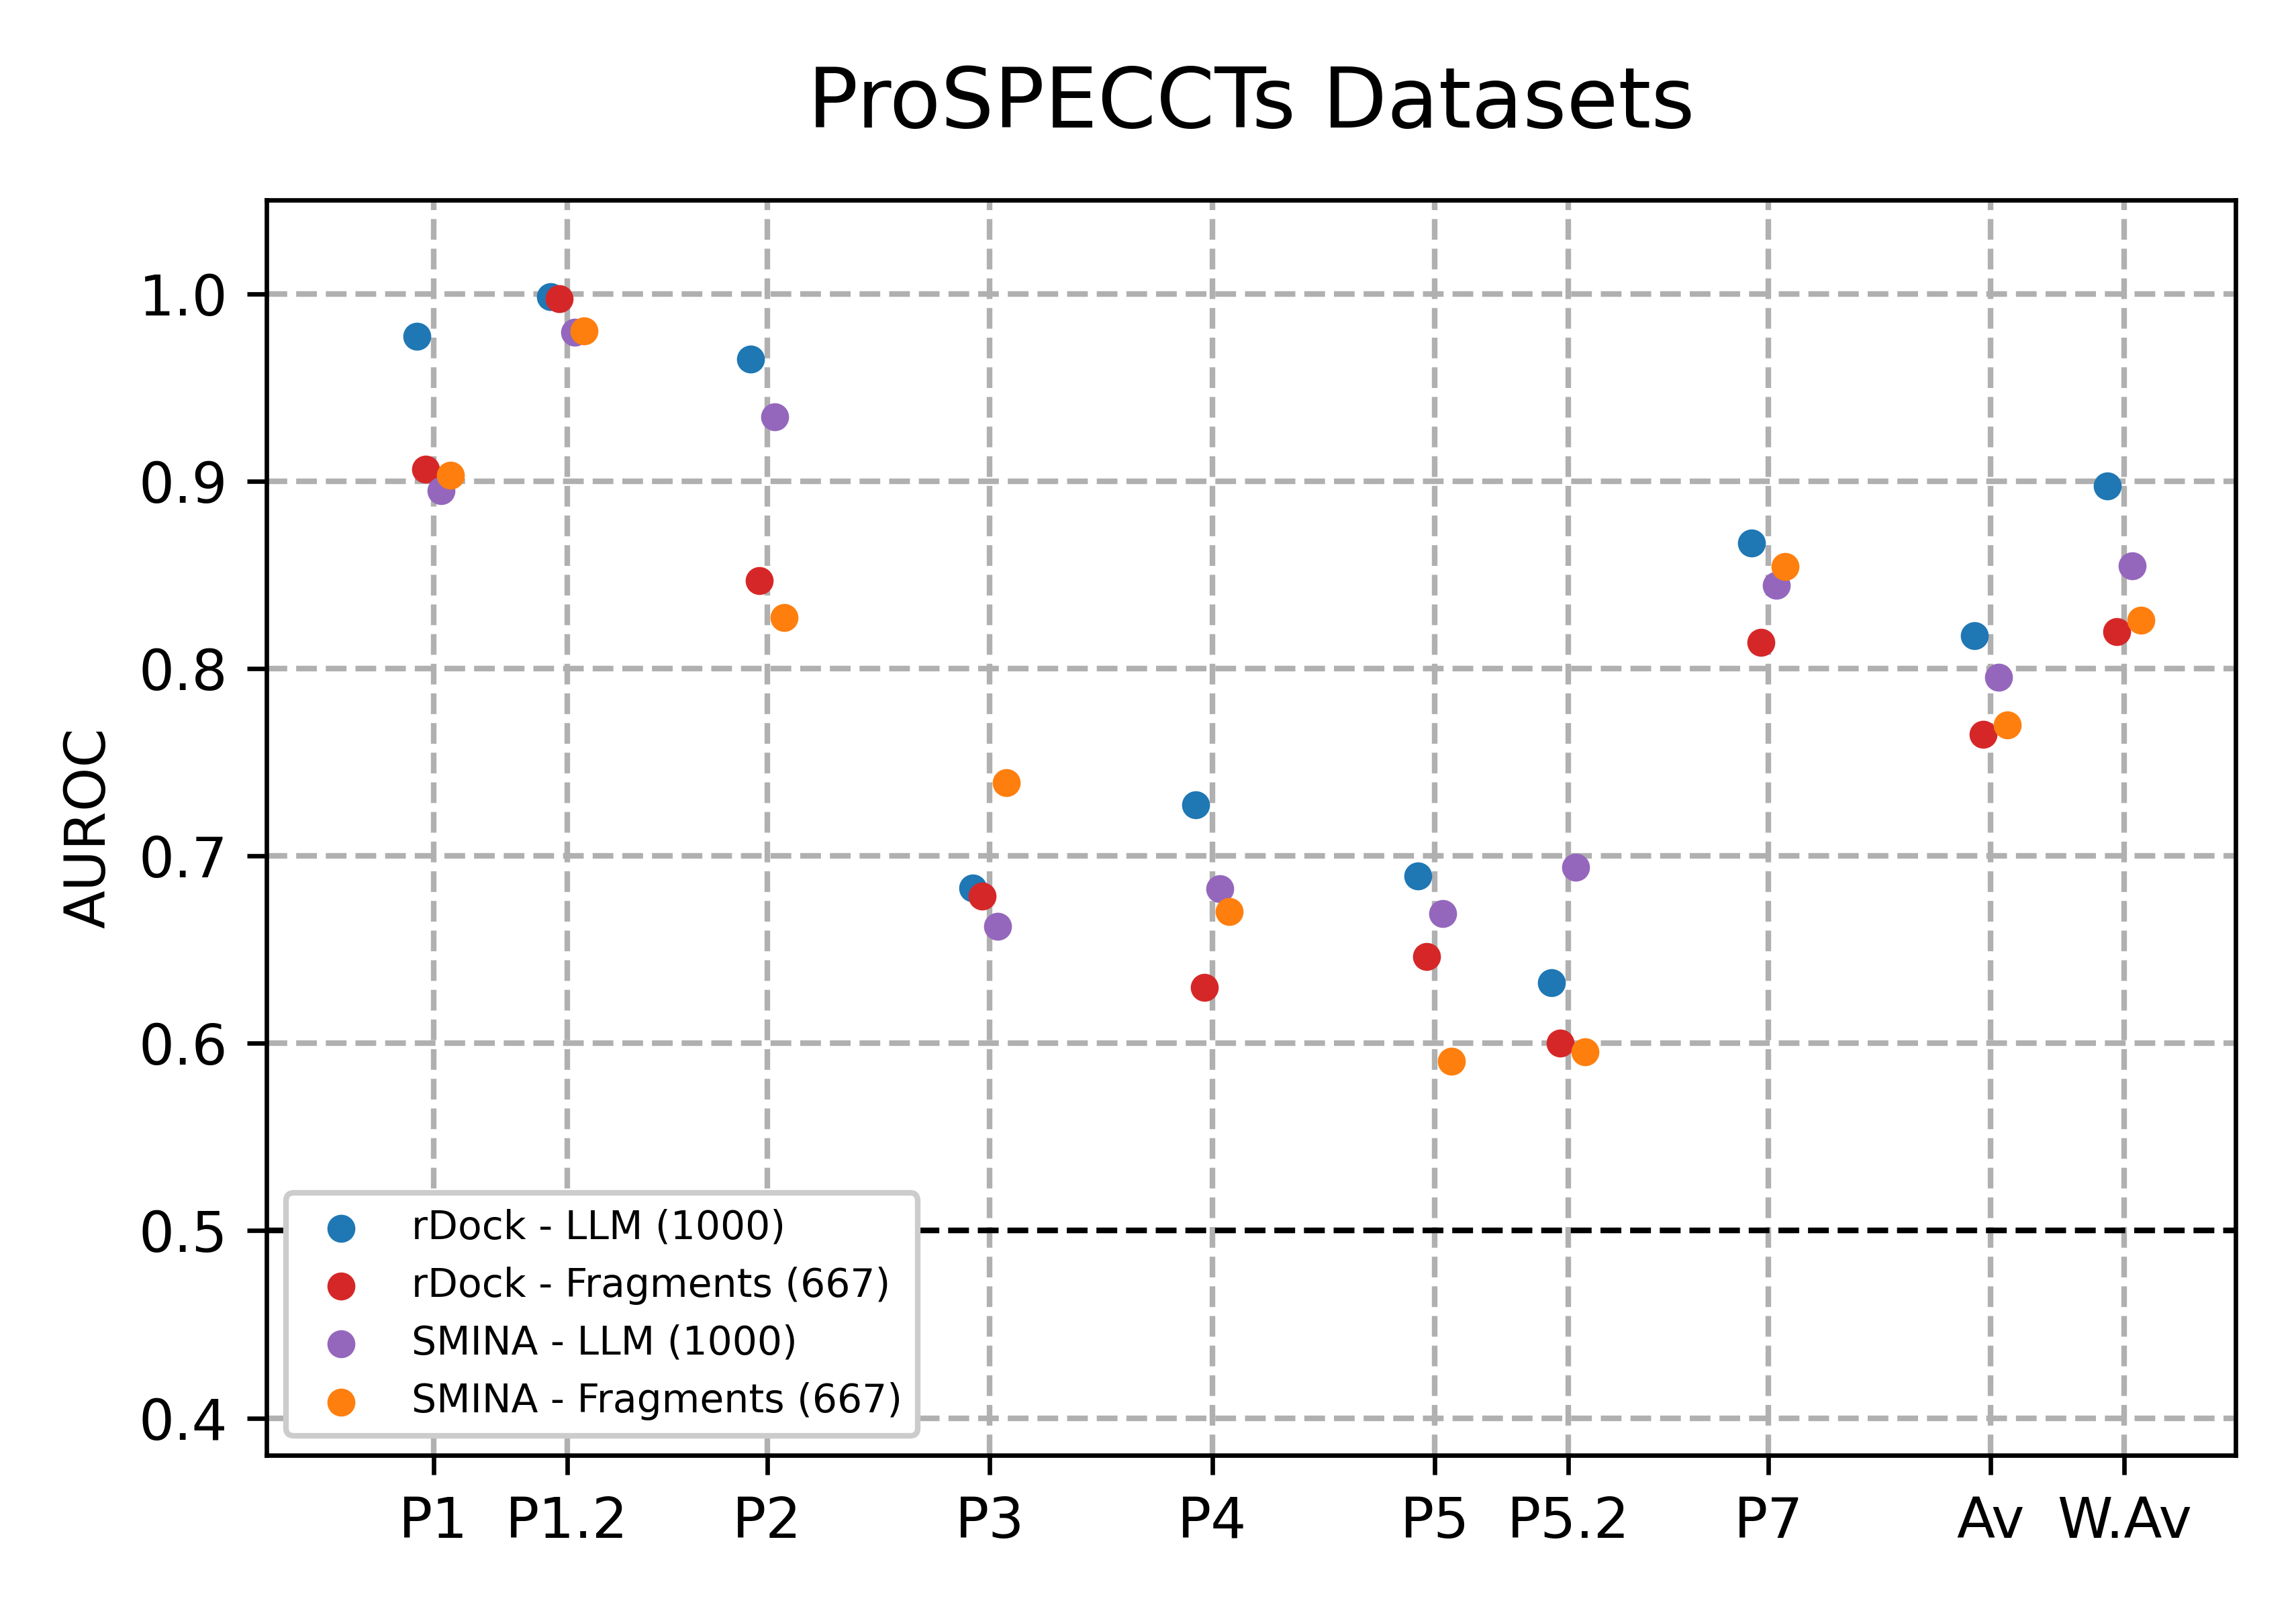
\includegraphics[width=0.65\linewidth]{figures/PocketVec/Supplementary/FigS4.png}
  \caption{
  Performances (AUROC, y-axis) among ProSPECCTs datasets (x-axis). Each colored dot represents the individual performance of our strategies with all possible combinations of docking approaches (rDock and SMINA) and compound collections (1,000 LLM and 667 fragments). Av. values represent the average performance among ProSPECCTs datasets for each individual strategy and W. Av. values weight the average value according to the number of pairs within each dataset.
  }
  \label{PocketVec_FigS4}
\end{figure}


\begin{figure}[htbp]
  \centering
  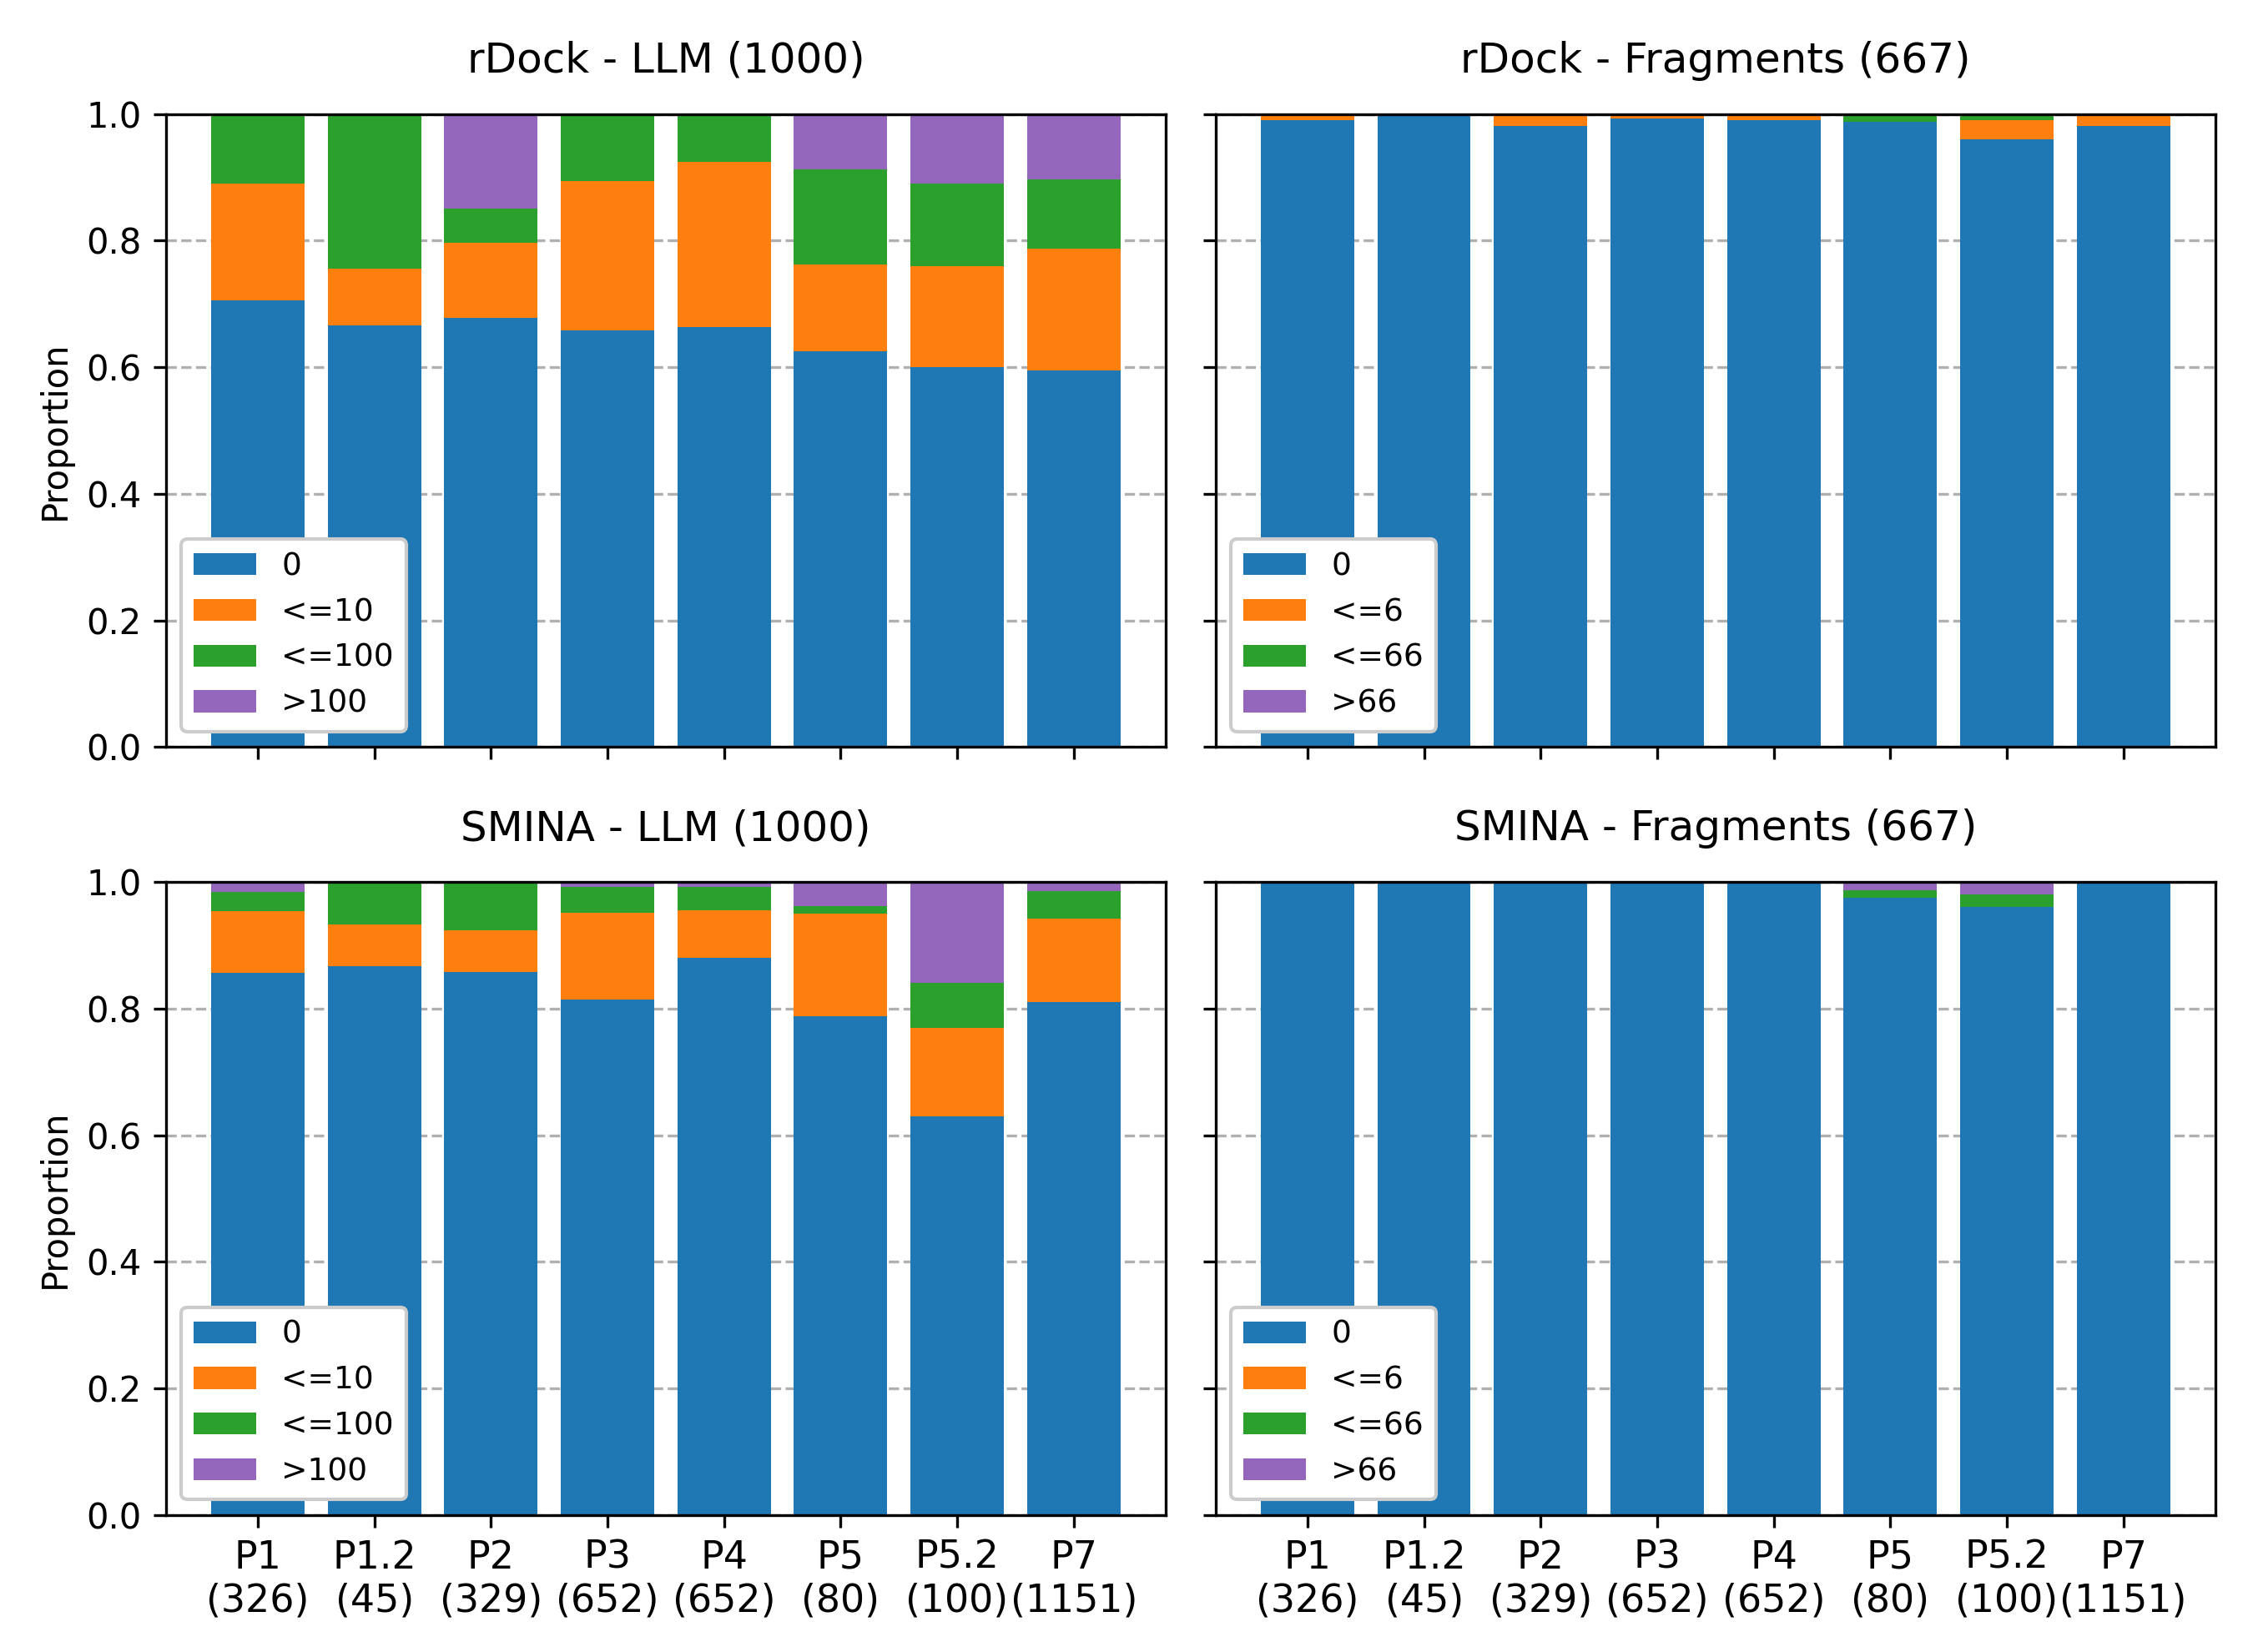
\includegraphics[width=0.75\linewidth]{figures/PocketVec/Supplementary/FigS5.png}
  \caption{
  Proportion of outlier molecules. Colored bars represent the proportion of outlier molecules (y-axis) within each ProSPECCTs dataset (x-axis) for each combination of docking method (rDock and SMINA) and compound collection (1,000 LLM and 667 fragments). Colors indicate the number of outlier molecules assigned to each structure. The number of structures per dataset is specified in parenthesis (x labels).
  }
  \label{PocketVec_FigS5}
\end{figure}

\begin{figure}[htbp]
  \centering
  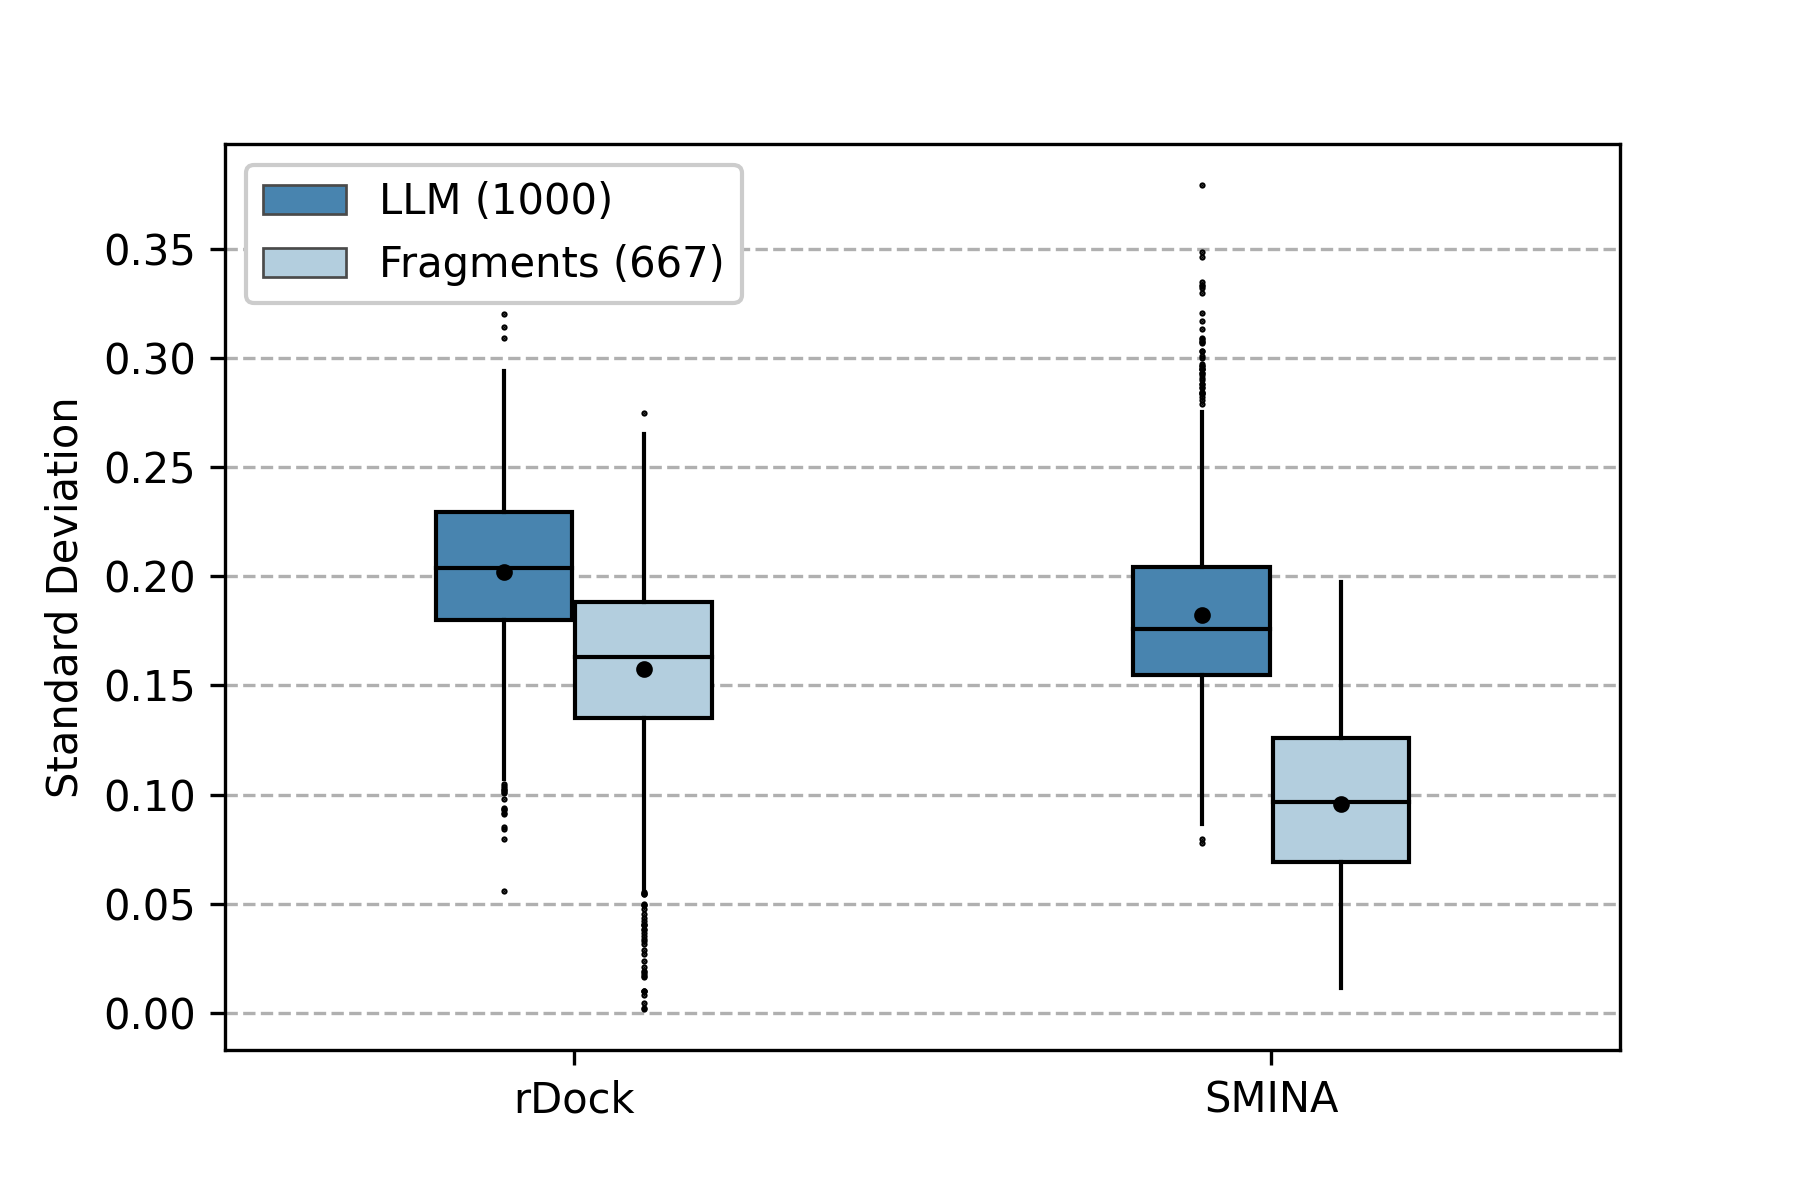
\includegraphics[width=0.55\linewidth]{figures/PocketVec/Supplementary/FigS6.png}
  \caption{
  Ranking diversity differences. For each docking method (rDock and SMINA) and compound collection (1,000 LLM and 667 fragments) ProSPECCTs pockets were considered all at once (3,335 pockets) and the standard deviation (in terms of rankings) was calculated for each tested compound. For both docking strategies standard deviation distributions between LLM and fragments are statistically different (Mann-Whitney U test, p<10-70 in both cases). Box plots indicate median (middle line), 25th, 75th percentile (box), and max and min value within the 1.5*25th and 1.5*75th percentile range (whiskers). Black dots represent mean values.
  }
  \label{PocketVec_FigS6}
\end{figure}


\begin{figure}[htbp]
  \centering
  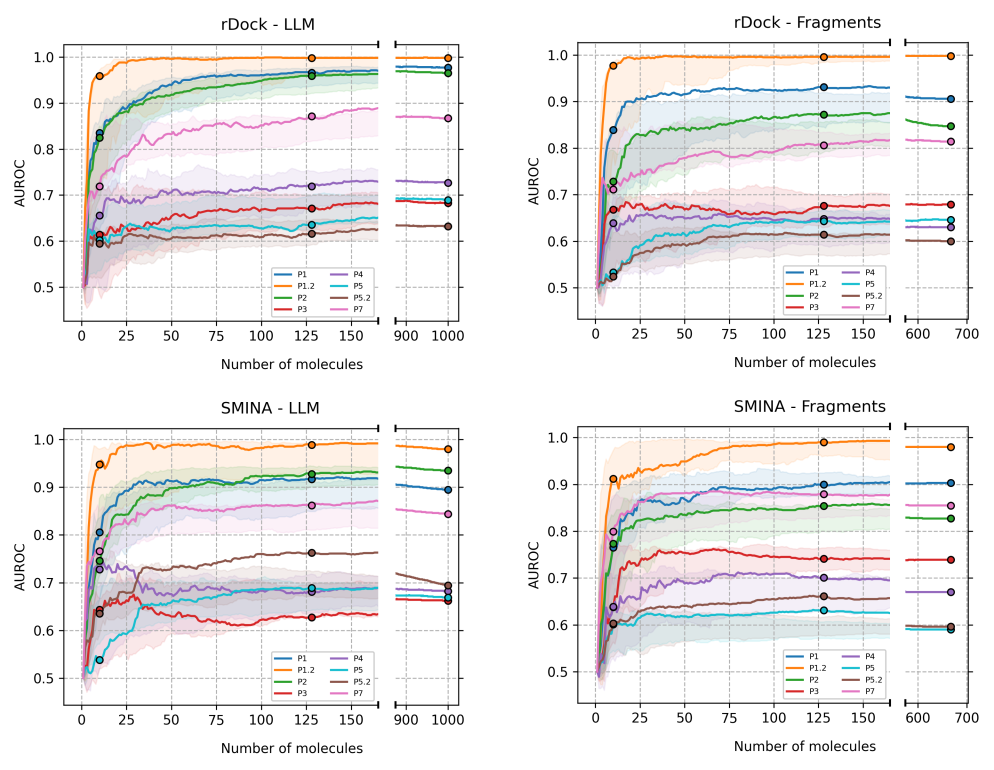
\includegraphics[width=1\linewidth]{figures/PocketVec/Supplementary/FigS7.png}
  \caption{
  Performances (AUROC, y-axis) of our descriptors among ProSPECCTs datasets (color, P6 and P6.2 not included. For further details, please see Online Methods) generated with a varying number of predefined compounds (x-axis, from 1 to complete sets, sorted by entropy). Colored points indicate the performance at 10, 128 and 1,000/667 molecules. Colored areas represent the best and worst performances obtained with randomly (x100) selected compounds (not sorted by entropy values). Each subplot corresponds to a combination of docking method (rDock and SMINA) and compound collection (1,000 LLM and 667 fragments).   
  }
  \label{PocketVec_FigS7}
\end{figure}

\begin{figure}[htbp]
  \centering
  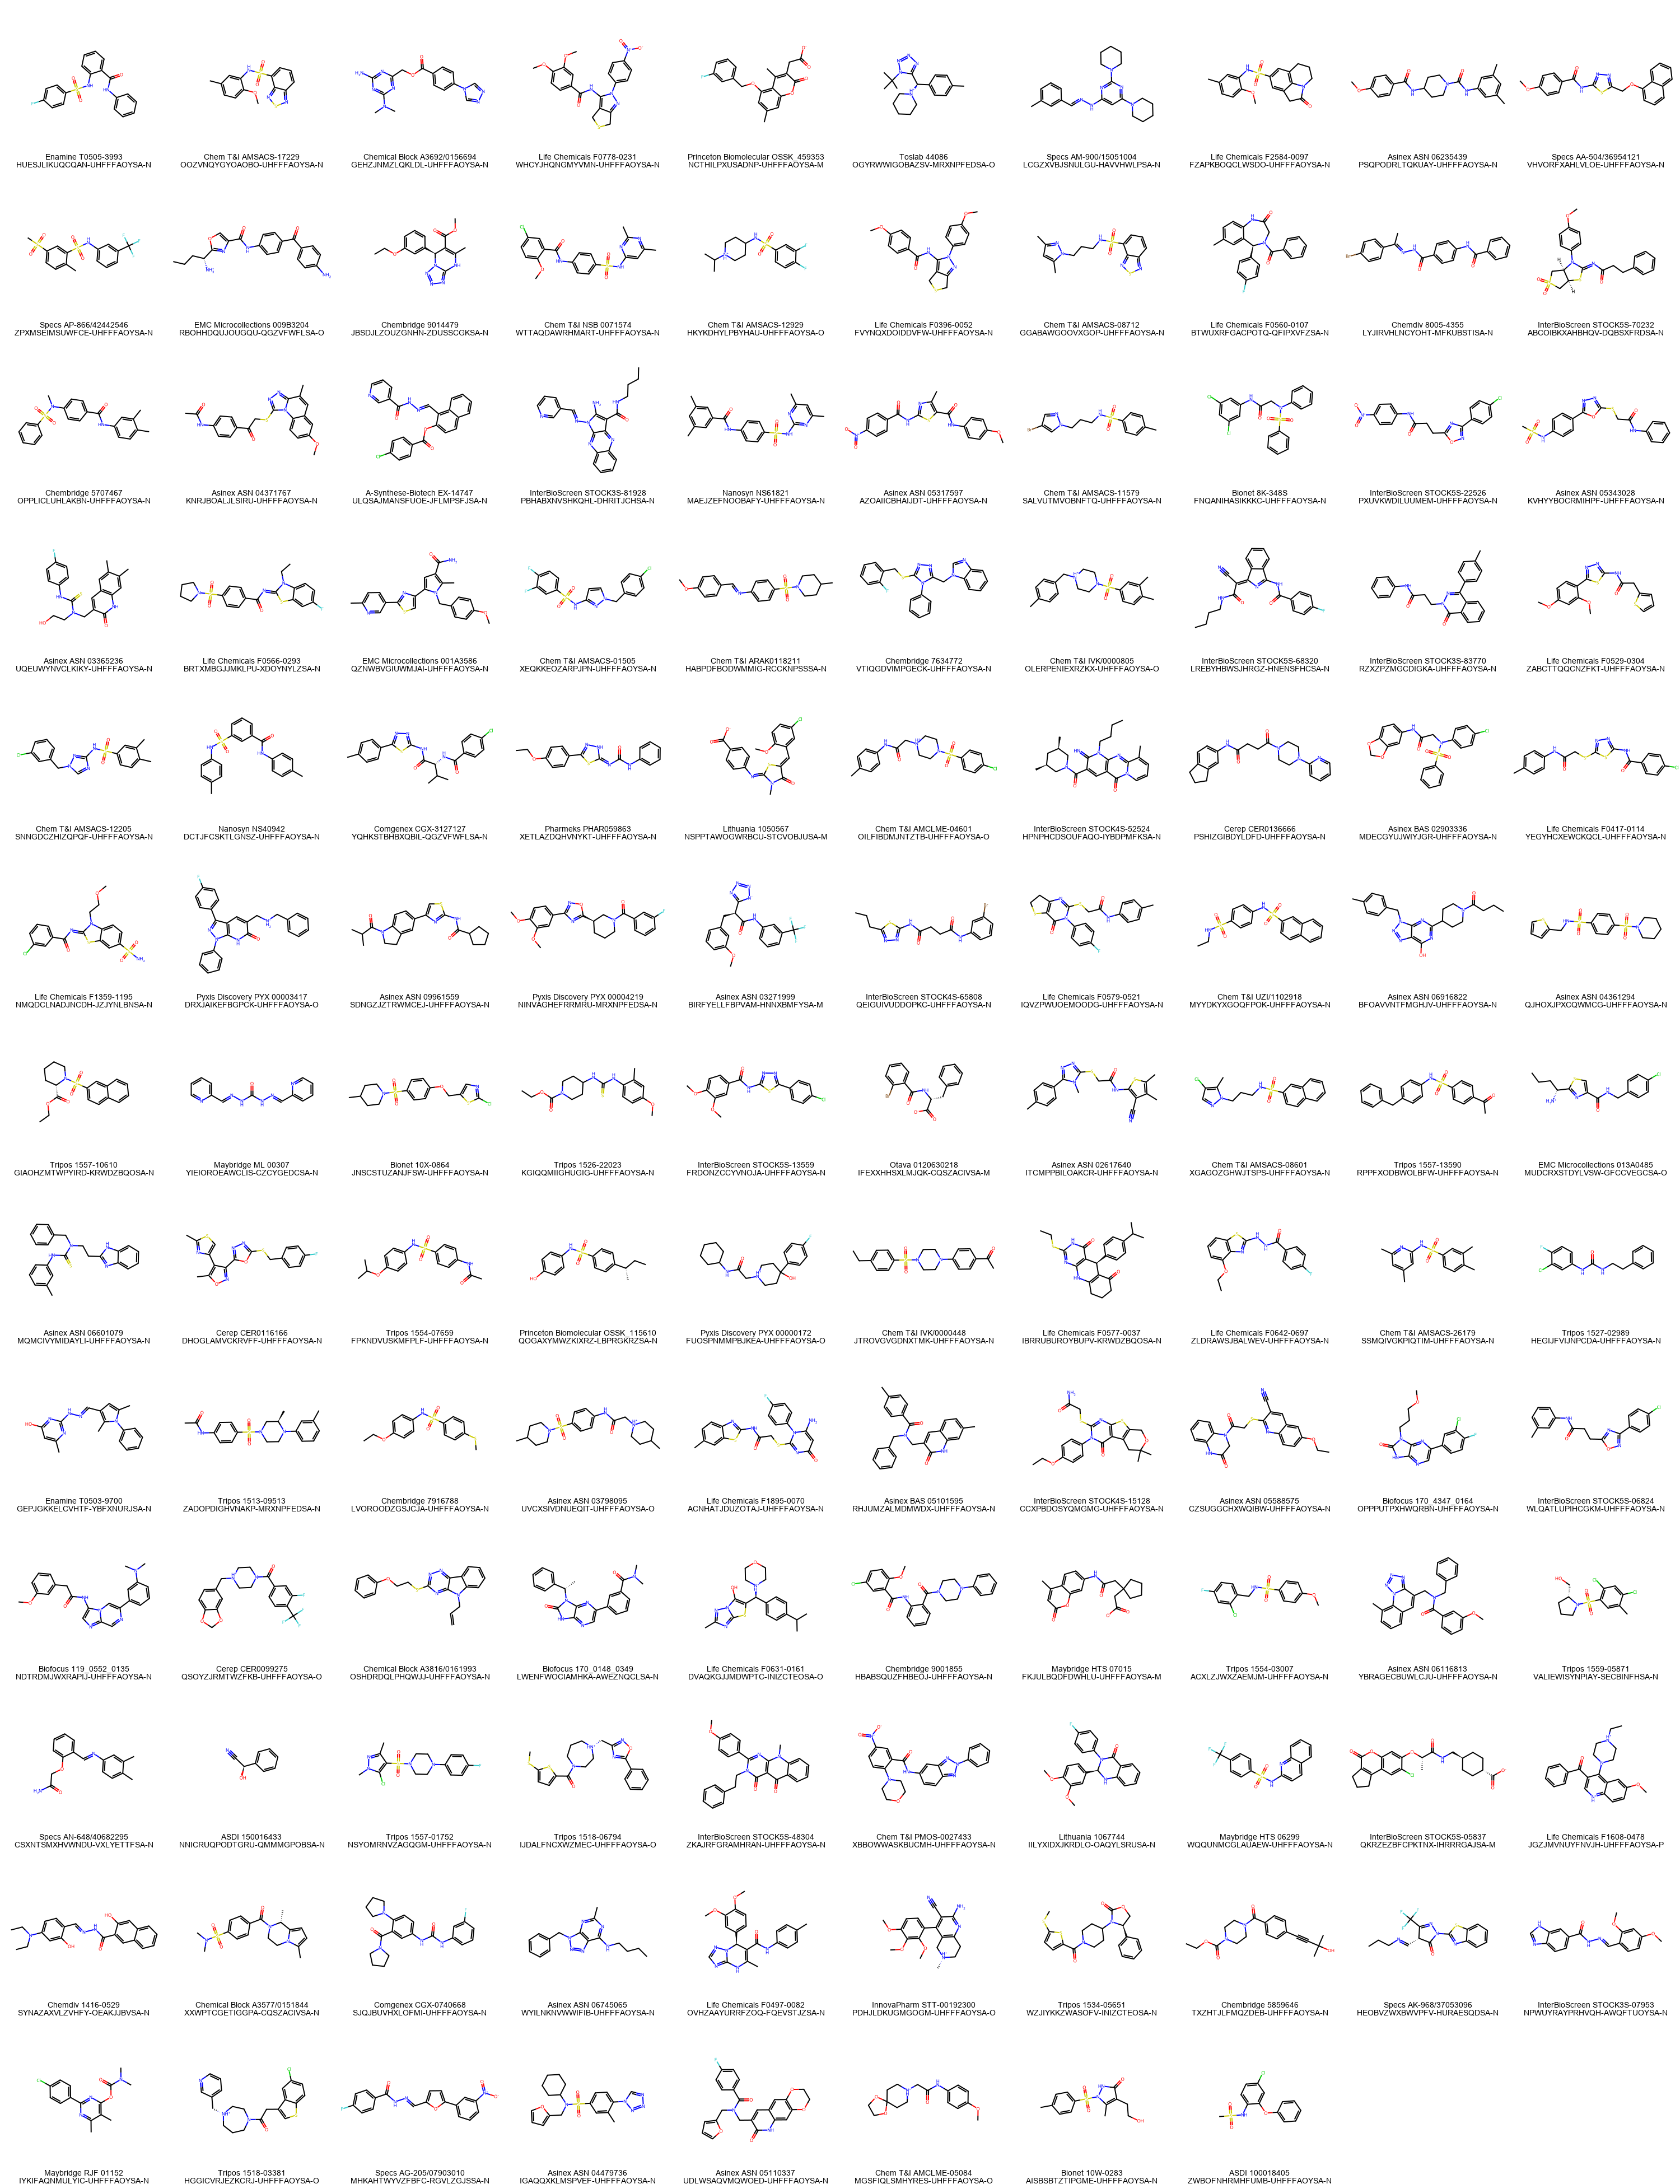
\includegraphics[width=0.9\linewidth]{figures/PocketVec/Supplementary/FigS8_v2.png}
  \caption{
  Standard 128 lead-like molecules used to generate PocketVec descriptors, including their commercial names and InChiKeys.
  }
  \label{PocketVec_FigS8_v2}
\end{figure}

\begin{figure}[htbp]
  \centering
  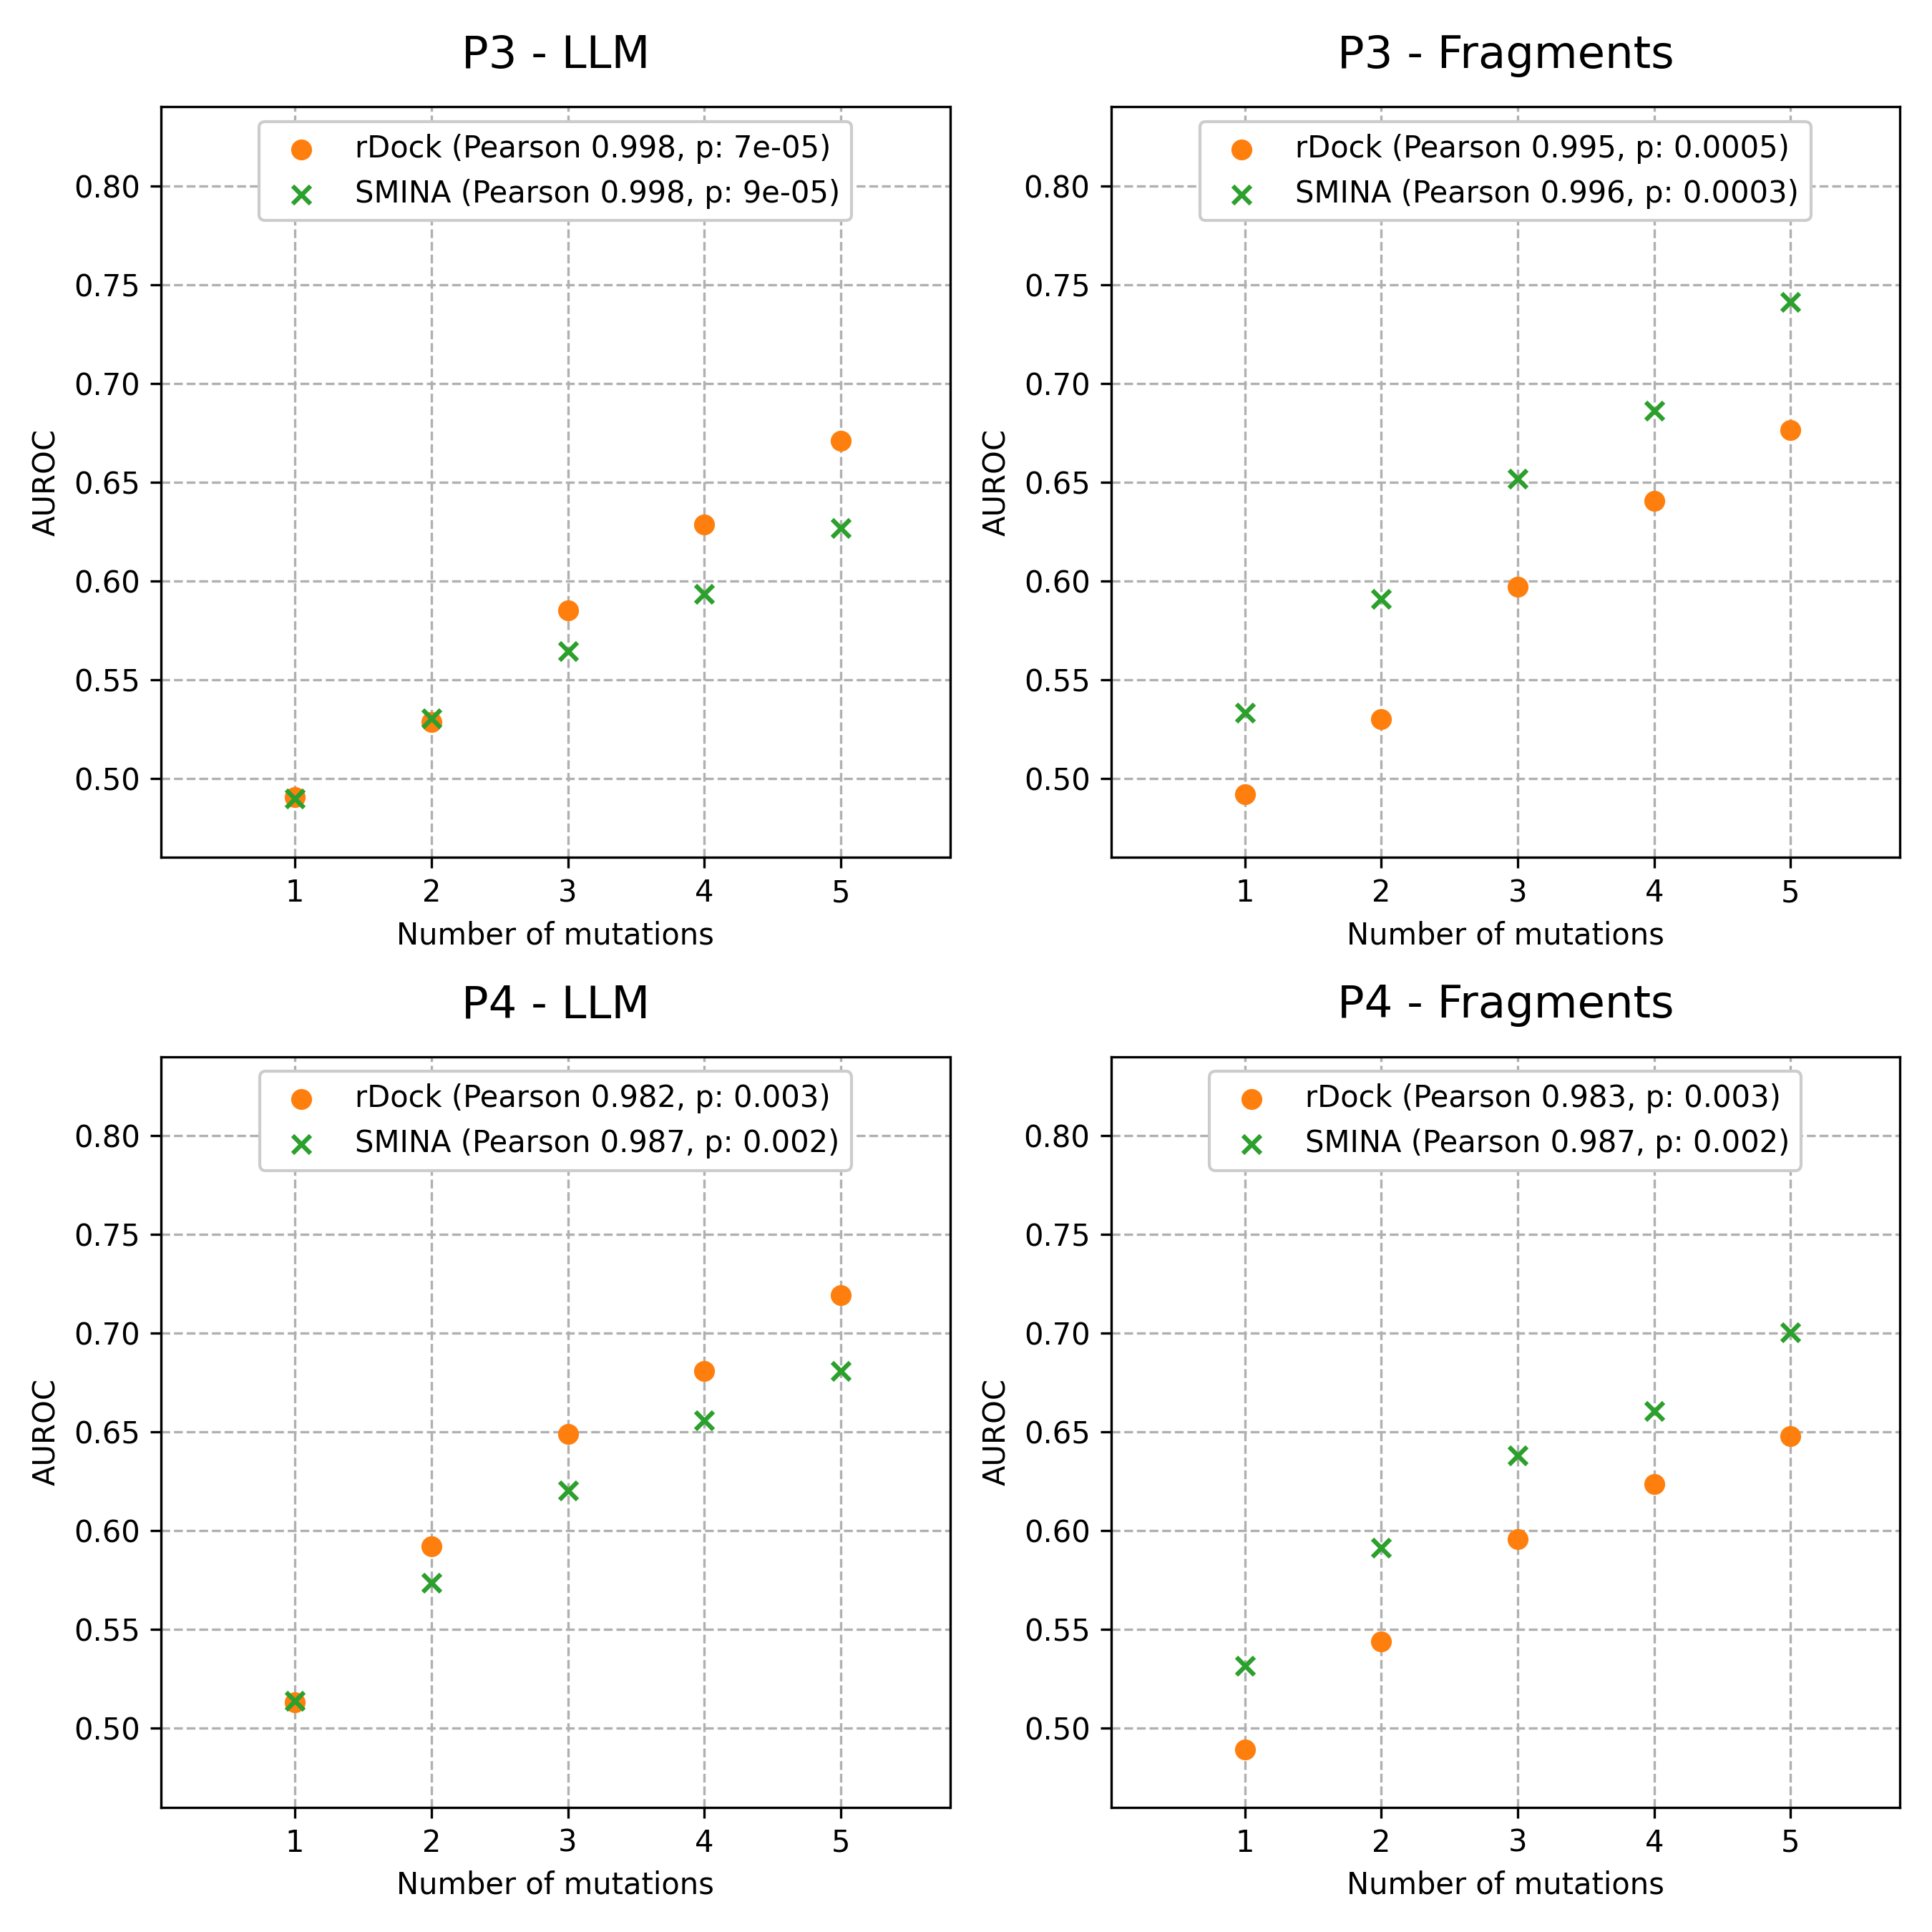
\includegraphics[width=0.8\linewidth]{figures/PocketVec/Supplementary/FigS9.png}
  \caption{
  Correlation between the AUROC (y-axis) and the number of artificial mutations (x-axis) in pocket-lining residues leading to changes in physicochemical properties (ProSPECCTs P3) and both physicochemical and shape properties (ProSPECCTs P4). Each subplot corresponds to a specific ProSPECCTs dataset (P3, P4) and collection of compounds (128 LLM and 128 fragments). Dot color and marker indicate the used docking method (rDock for rigid docking and SMINA for flexible docking). In the legend, the corresponding Pearson’s Correlation Coefficients are reported. 
  }
  \label{PocketVec_FigS9}
\end{figure}

\begin{figure}[htbp]
  \centering
  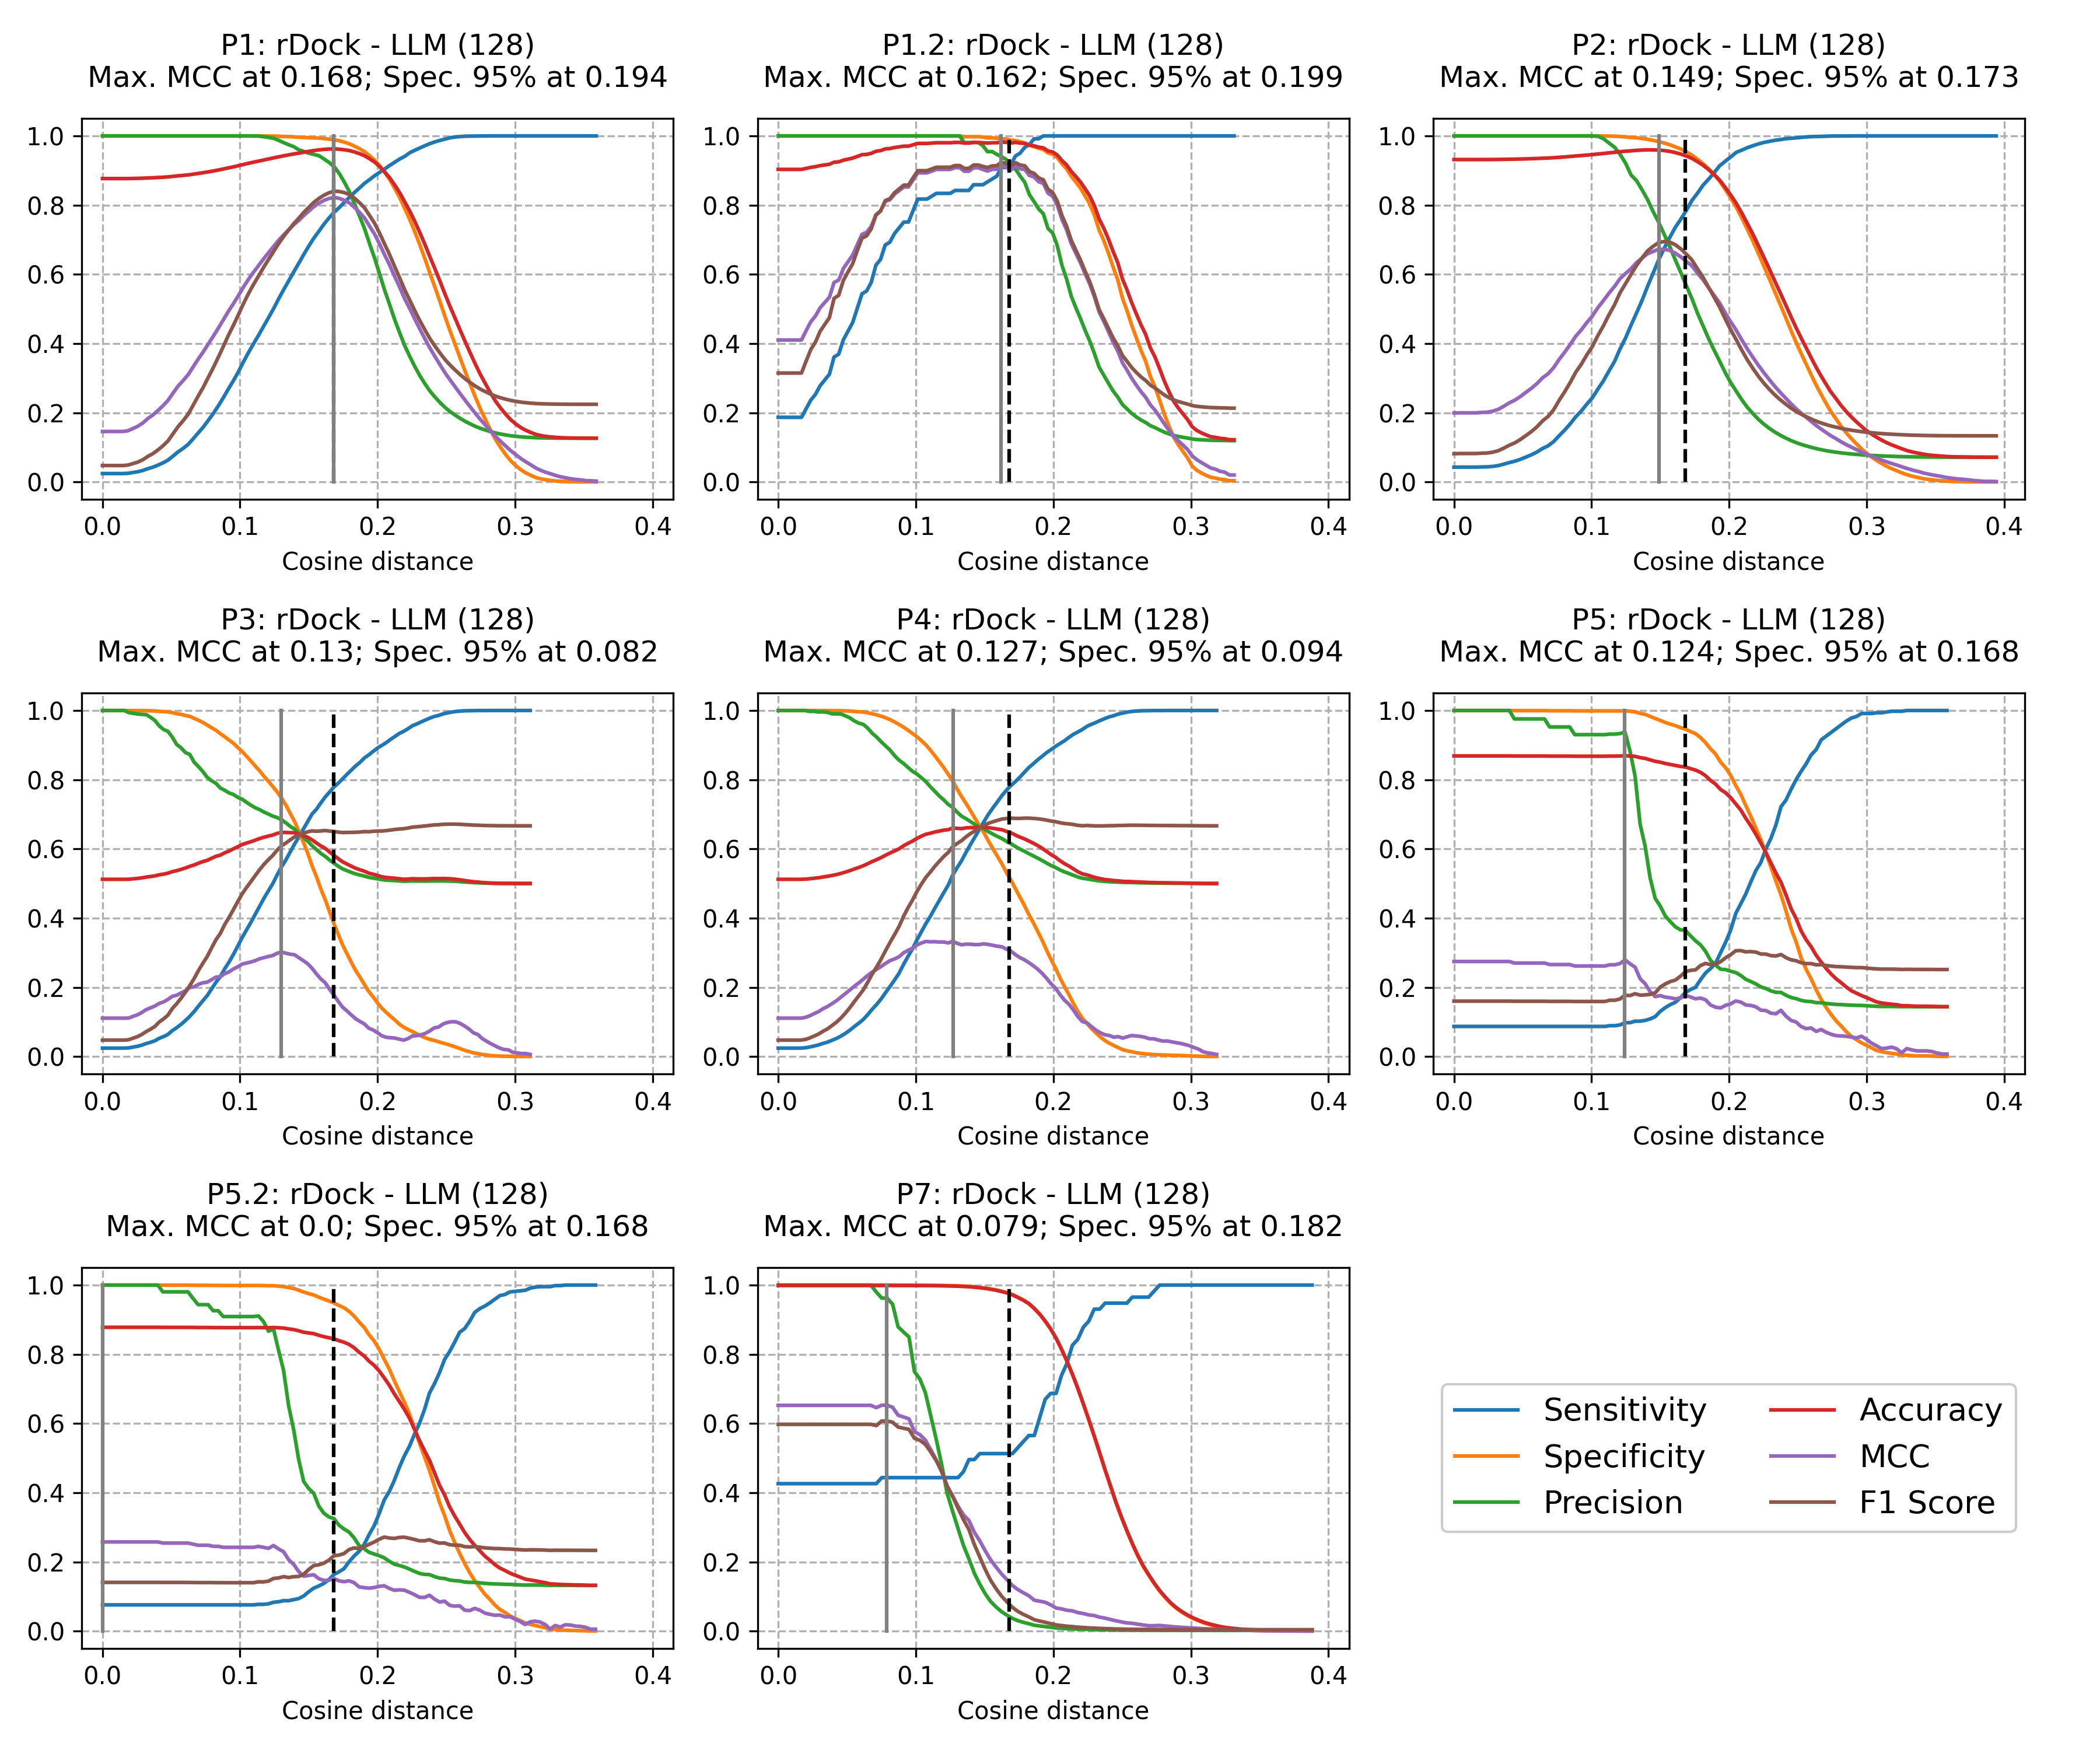
\includegraphics[width=\linewidth]{figures/PocketVec/Supplementary/FigS10_v2.png}
  \caption{
  For each ProSPECCTs dataset, evolution (y-axis) of the Sensitivity (blue), Specificity (orange), Precision (green), Accuracy (red), MCC (purple) and F1 Score (brown) at different distance threshold values (x-axis, cosine distance). The vertical gray thin line represents the cosine distance maximizing the MCC in each ProSPECCTs dataset. The vertical dashed black line represents the cosine distance maximizing the MCC in ProSPECCTs P1 (0.17), which corresponds to the general guideline for classifying a pocket pair of interest as either similar or dissimilar.
  }
  \label{PocketVec_FigS10}
\end{figure}



% \begin{figure}[htbp]
%   \centering
%   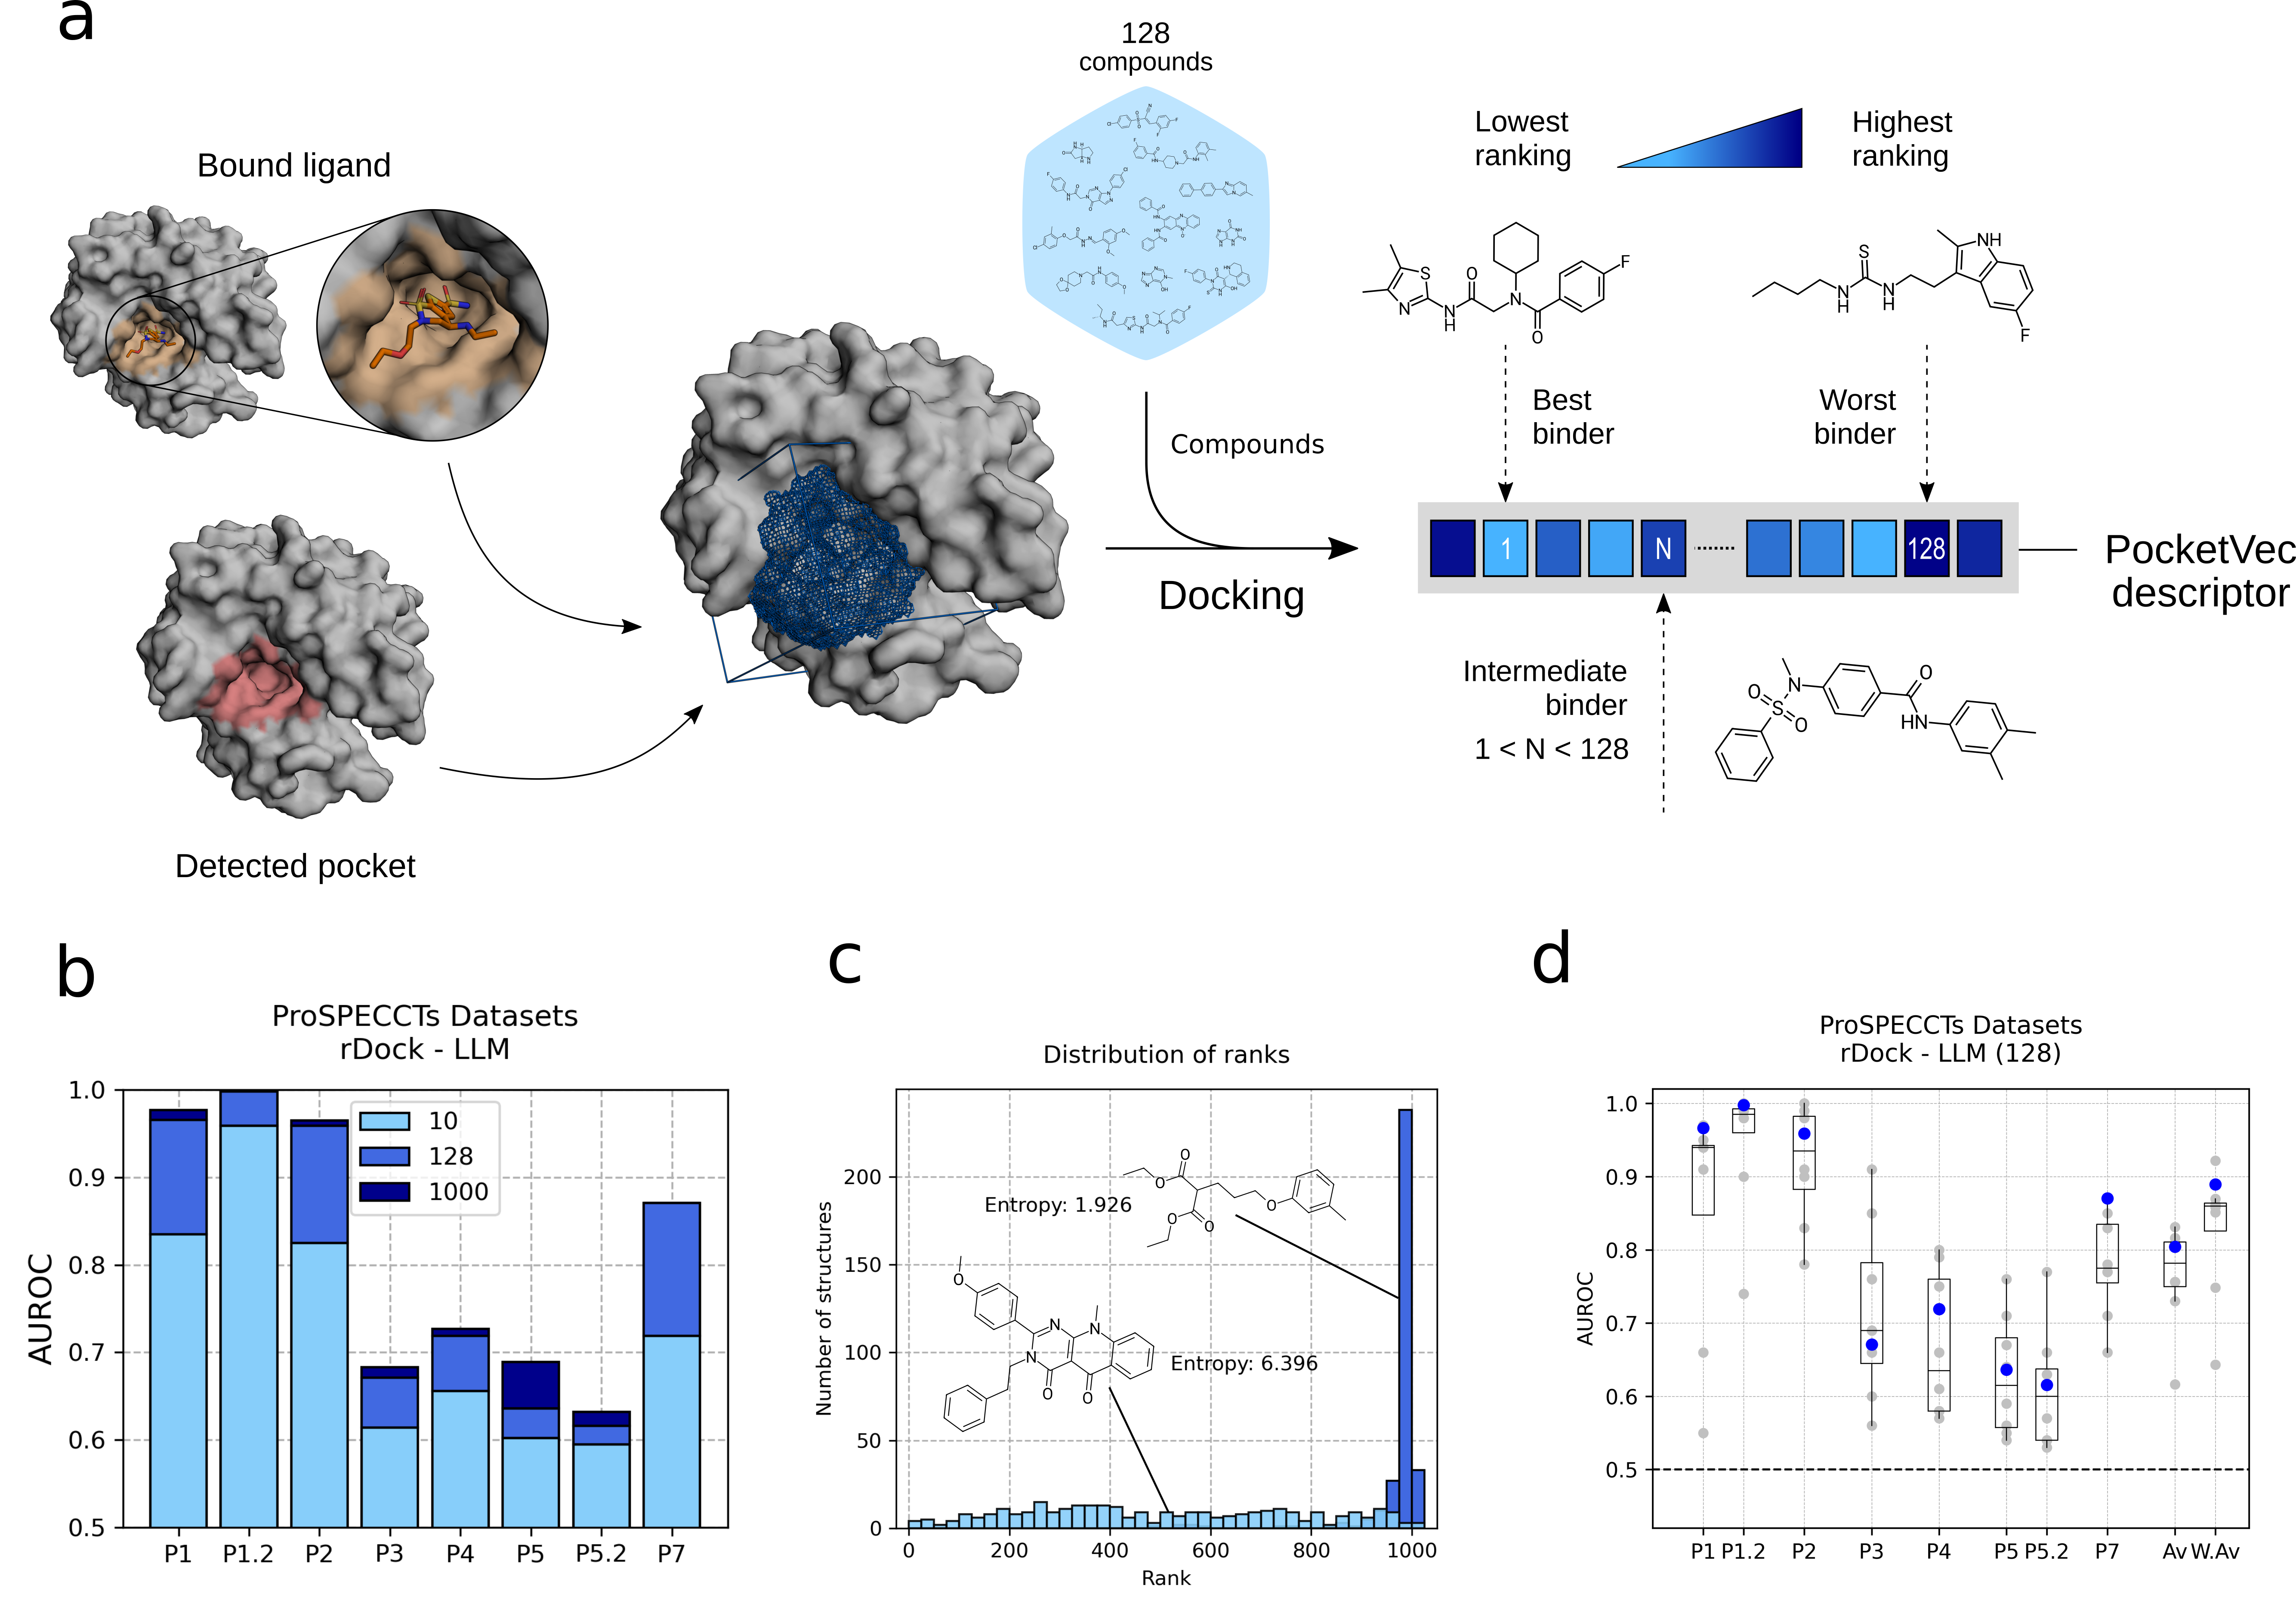
\includegraphics[width=\linewidth]{figures/PocketVec/Main/Fig1.png}
%   \caption{
  
%   }
%   \label{Fig1}
% \end{figure}




%%%%%%%%%%%%%%%%%%%%
%%%%  TABLES  %%%%%%
%%%%%%%%%%%%%%%%%%%%

\newpage

\renewcommand{\thetable}{A.\arabic{section}.\arabic{table}}
\counterwithin{table}{section}
\setcounter{section}{4}
\setcounter{table}{0}

% Define a new column type for tabularx that allows line breaks and centers the text
\newcolumntype{C}[1]{>{\centering\arraybackslash}m{#1}}

% Importing and displaying the CSV file as a table
\csvreader[
    longtable=|C{1.8cm}|C{0.8cm}|C{0.8cm}|C{0.8cm}|C{0.8cm}|C{0.8cm}|C{0.8cm}|C{0.8cm}|C{0.8cm}|C{0.8cm}|C{0.8cm}|C{0.8cm}|,  % Adjust the widths as needed
    table head=\caption{Performances (AUROCs) of existing strategies (Deeplytough\cite{simonovsky_deeplytough_2020}, FuzCav\cite{weill_alignment-free_2010}, SiteAlign\cite{schalon_simple_2008}, KRIPO\cite{wood_pharmacophore_2012}, TIFP\cite{desaphy_encoding_2013}, BindSiteS-CNN\cite{scott_classification_2022}. File format is specified if needed) to compare pockets based on pocket descriptors/fingerprints among ProSPECCTs datasets. TOP-3 rows include the number of pairs within each dataset together with the best performing method. Median and Average performances have been calculated without considering PocketVec results (colored).
    }\label{PocketVec_TableS1} \\\toprule & \textbf{D1} & \textbf{D1.2} & \textbf{D2} & \textbf{D3} & \textbf{D4} & \textbf{D5} & \textbf{D5.2} & \textbf{D7} & \textbf{Av} & \textbf{W. Av.} \\\midrule\endfirsthead
    \toprule & \textbf{D1} & \textbf{D1.2} & \textbf{D2} & \textbf{D3} & \textbf{D4} & \textbf{D5} & \textbf{D5.2} & \textbf{D7} & \textbf{Av} & \textbf{W. Av.} \\\midrule\endhead
    \bottomrule\endfoot,
    before reading={\catcode`\#=12}, % Handle special characters
    late after line=\\\midrule,
]{figures/PocketVec/Supplementary/TableS1.csv}{} % Path to your CSV file
{%
    \ifthenelse{\equal{\csvcoli}{Best Method(s)}}%
    {\small \csvcoli & \tiny \csvcolii & \tiny \csvcoliii & \tiny \csvcoliv & \tiny \csvcolv & \tiny \csvcolvi & \tiny \csvcolvii & \tiny \csvcolviii & \tiny \csvcolix & \tiny \csvcolx & \tiny \csvcolxi}%
    {\ifthenelse{\equal{\csvcoli}{PocketVec}}%
        {\small \textcolor{SchoolColor}{\csvcoli} & \textcolor{SchoolColor}{\csvcolii} & \textcolor{SchoolColor}{\csvcoliii} & \textcolor{SchoolColor}{\csvcoliv} & \textcolor{SchoolColor}{\csvcolv} & \textcolor{SchoolColor}{\csvcolvi} & \textcolor{SchoolColor}{\csvcolvii} & \textcolor{SchoolColor}{\csvcolviii} & \textcolor{SchoolColor}{\csvcolix} & \textcolor{SchoolColor}{\csvcolx} & \textcolor{SchoolColor}{\csvcolxi}}%
        {\small \csvcoli & \csvcolii & \csvcoliii & \csvcoliv & \csvcolv & \csvcolvi & \csvcolvii & \csvcolviii & \csvcolix & \csvcolx & \csvcolxi}%
    }%
}










\chapter{Publications}
\newpage
\section{List of publications}
\section{Attachment of publications}


\end{appendices}


% % Include PDFs
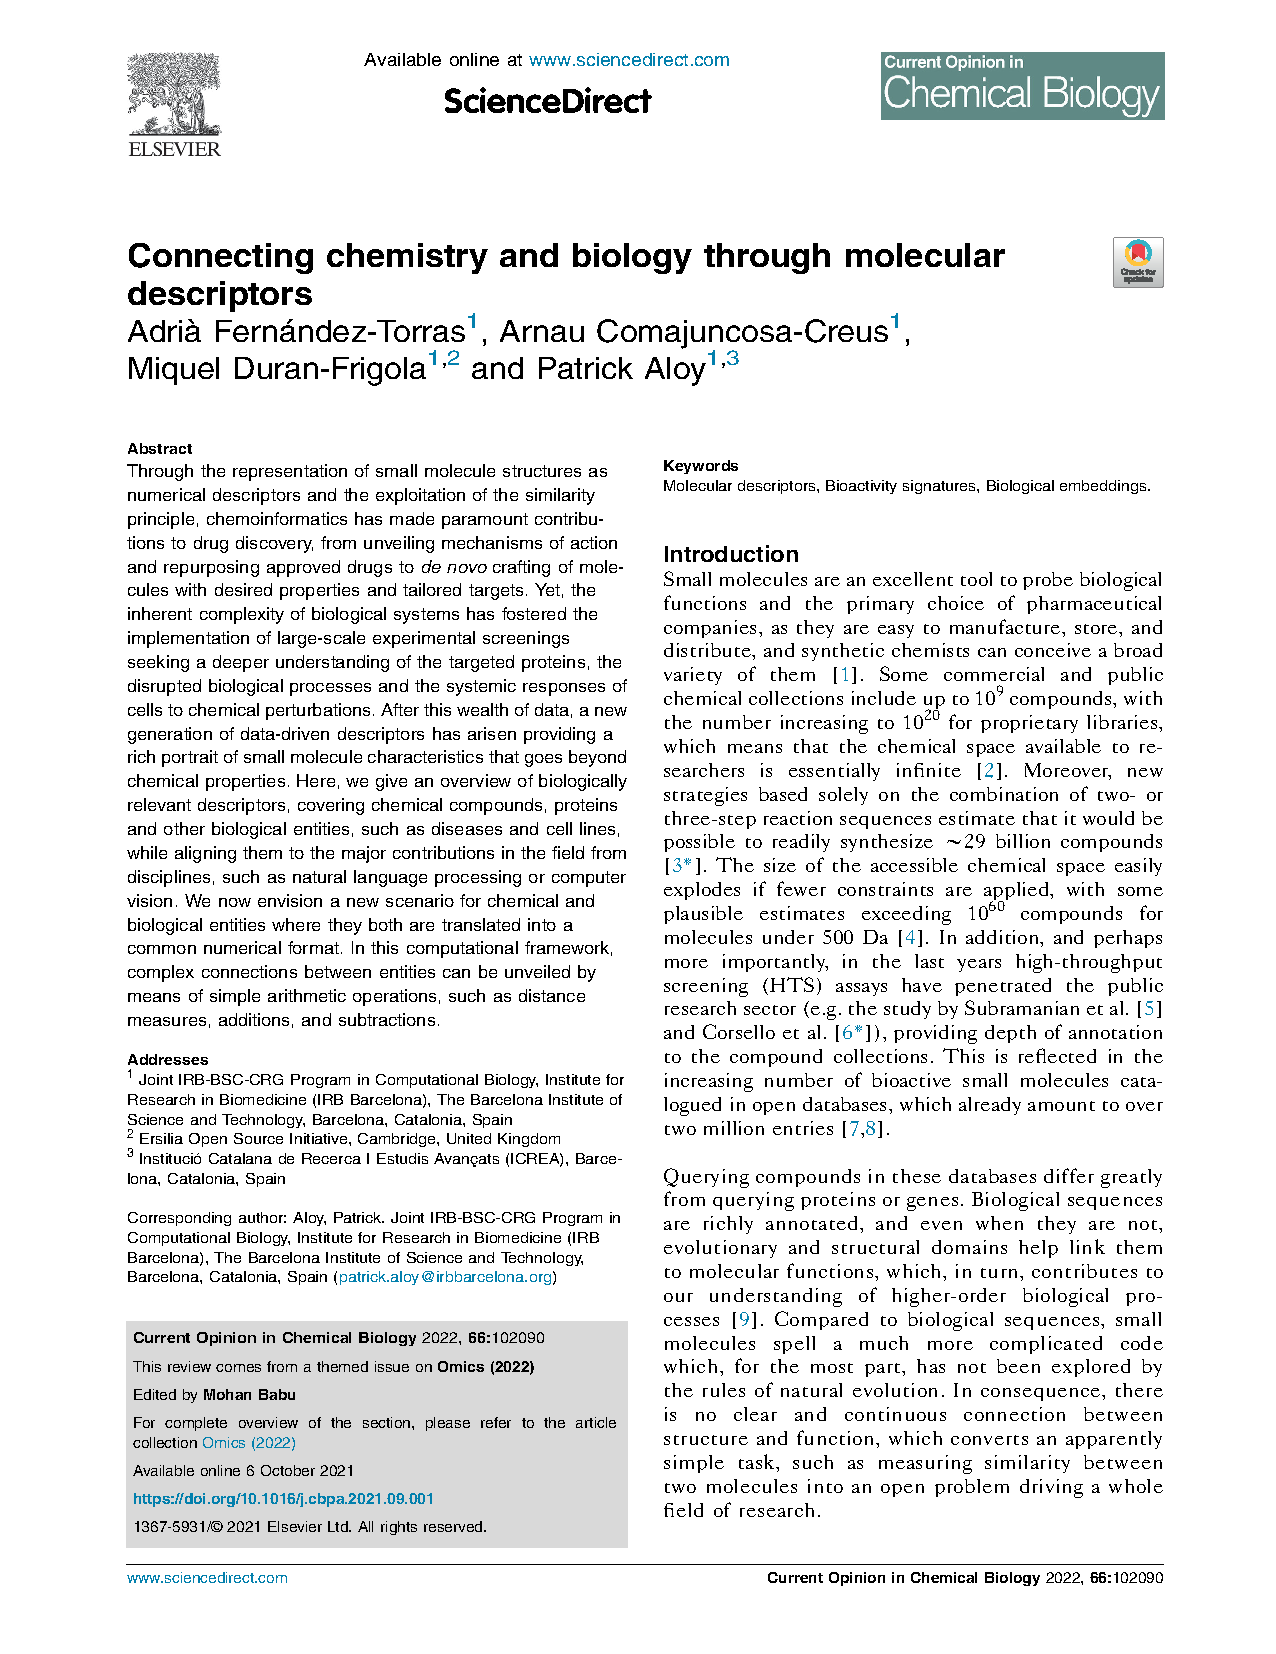
\includepdf[pages=-]{PDFs/COCB.pdf}
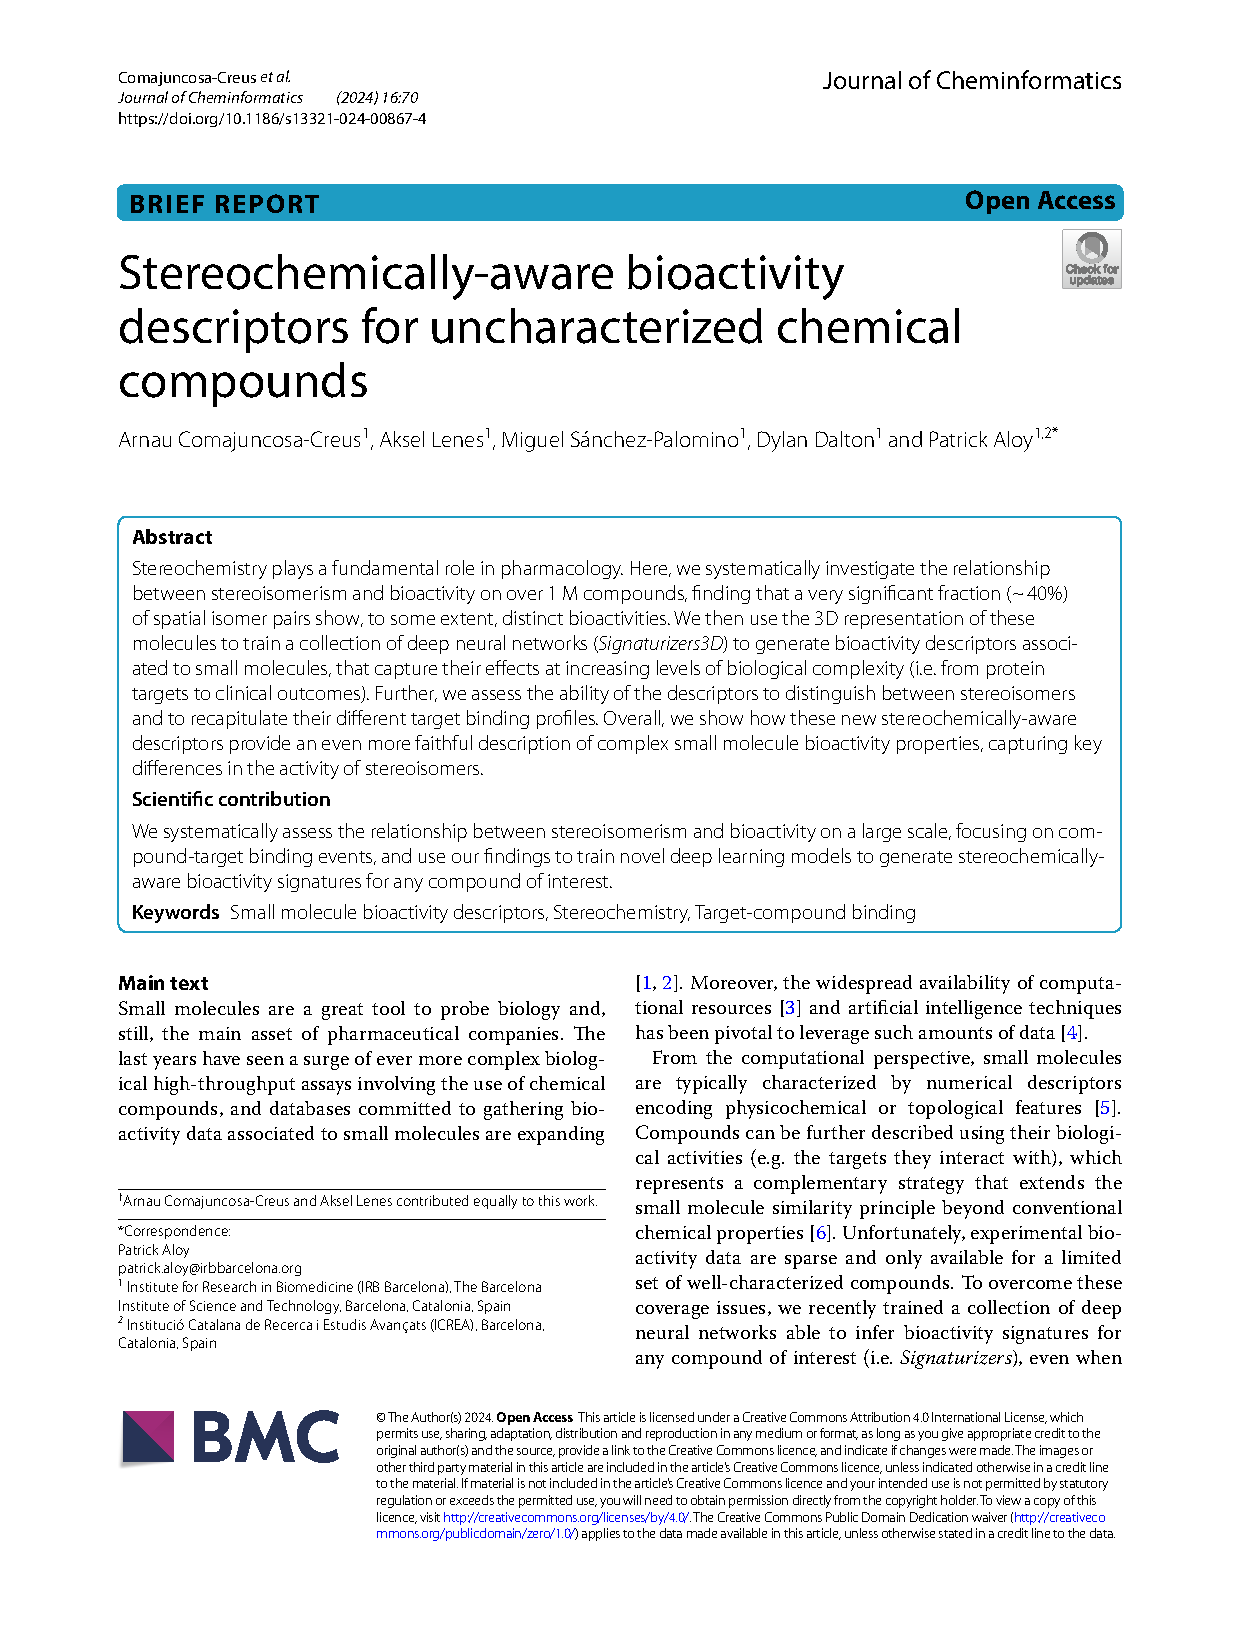
\includepdf[pages=-]{PDFs/sign3D.pdf}
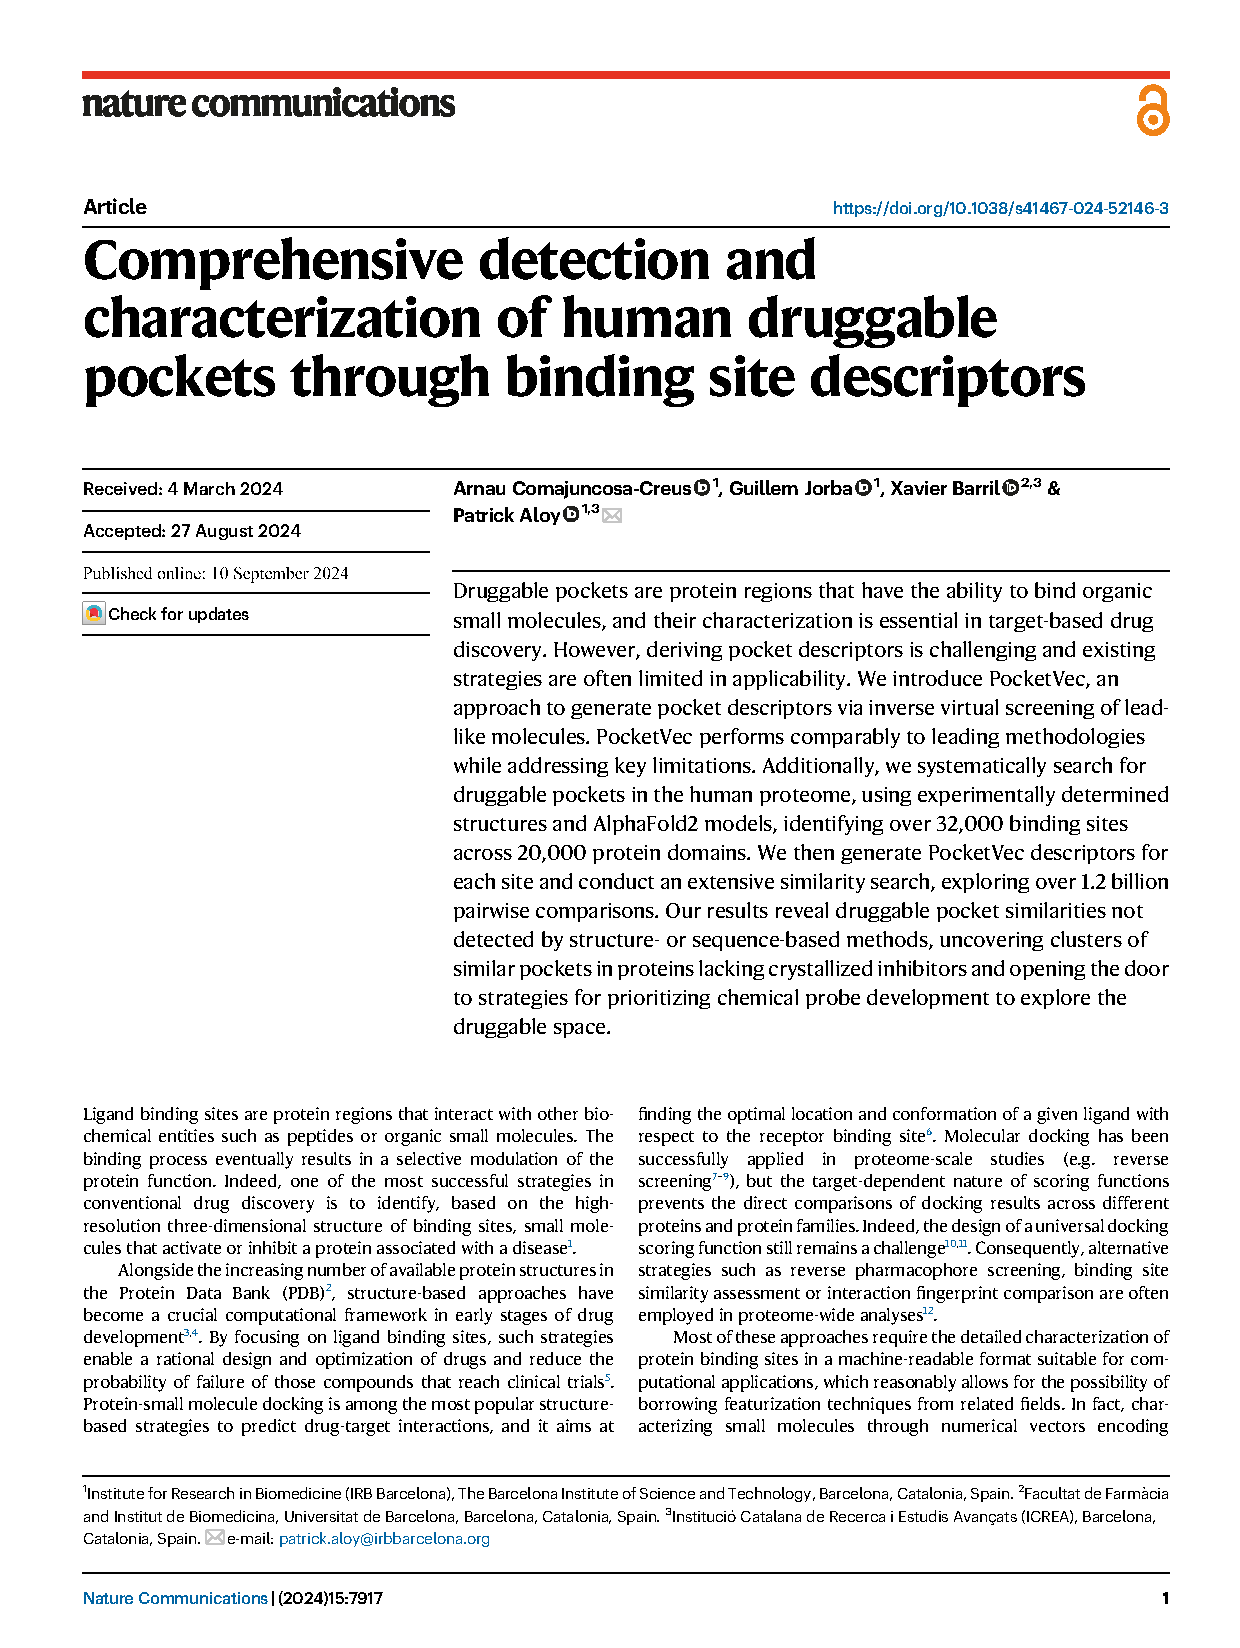
\includepdf[pages=-]{PDFs/PocketVec.pdf}

\newpage
% dedication text

\newpage
\vspace*{2cm}
\pagestyle{empty}
\begin{center}
    ``Deien «estimeu, perdeu el seny, jugueu fort, \\
    feu un gran ridícul, blasfemeu, desafieu la sort!»'' \\
    \vspace{0.3cm}
    -- M'hi vaig llençar, \textsc{Manel} \\
    \vspace{3cm}
    I, sobretot, sigueu lleials als altres. 
\end{center}



\newpage
\thispagestyle{empty}
\mbox{}
\newpage

\newpage
\thispagestyle{empty}
\mbox{}
\newpage

\end{document}